% !Mode:: "TeX:UTF-8" 
\chapter{绪论}[Example]

\section{课题背景及研究目的和意义}[Number]
生物通路是细胞中分子间的一系列活动,导致细胞内某种产物或变化。生物通路可以导致新的分子的组装(如脂肪和蛋白质)、控制基因的表达、刺激细胞的移动等\footnote{http://www.genome.gov/27530687}。复杂疾病往往和生物通路网络之间存在密切的关系。复杂疾病诸如糖尿病、癌症、心脏病,高血压等与多种致病基因、蛋白、生物通路网络是相互关联的\cite{jin2011systematic}。因此深入研究生物通路网络对于探索疾病的发病机制具有重要的意义和研究价值。随着高通量技术的发展和大量生物实验的开展,基因、蛋白、代谢等组学数据日益积累,研究人员推出了一批高质量的生物通路数据库如KEGG\cite{kanehisa2008kegg}(一种受到广泛欢迎的被生物学家广泛使用的数据库)、Reactome\cite{croft2013reactome}(一个免费的和手工标注生物通路的在线数据库);DrugBank\cite{wishart2006drugbank}(一种综合性的包含大量的药物和靶点数据以及生物通路数据的数据库)等(见表\ref{table1} )。这些数据库蕴含着大量通路、疾病、药物等信息,诸如疾病致病基因,分子间的作用信息,通路网络的拓扑结构等,对于这些数据的深入研究和挖掘对揭示复杂疾病发病机理,发现药物靶点等方面具有重要的意义。

\begin{table}[htbp]
  \centering
	\caption[table1]{常用的通路数据库及网址}
\vspace{0.5em}\wuhao
\begin{tabularx}{1.0\textwidth}{lXXl}
\toprule[1.5pt]
数据库名 & 简介 & 网址 & 参考文献\\
\midrule[1pt]
KEGG & 被生物学家广泛使用的通路数据库 & http://www.kegg.jp & \cite{kanehisa2008kegg} \\
Reactome	& 免费的和手工标注生物通路的在线数据库	& https://reactome.org & \cite{croft2013reactome} \\
WikiPathways	& 使用了维基百科概念的通路数据	& https://www.wikipathways.org & \cite{pico2008wikipathways} \\
PhosphoSitePlus	& 包含小鼠和人类的通路数据的数据库 & https://www.phosphosite.org &	\cite{hornbeck2011phosphositeplus} \\
BioCyc 	& 基因组通路数据库& https://biocyc.org/	& \cite{krummenacker2005querying} \\
PANTHER	& 基因及其产物相关的通路数据库&http://www.pantherdb.org	& \cite{mi2016panther} \\
\bottomrule[1.5pt]
\end{tabularx}
\end{table}

生物通路网络通常和多种疾病、药物、靶点等数据关联,为发现与已知的通路网络关联的药物、靶点、基因关系等,需要对已知的生物通路网络进行扩展。通路网络的常见的扩展方法是将生物通路数据映射到其他生物网络(如疾病、基因、药物网络)上,作为种子节点进行扩展(如图\ref{fig1}所示)。图\ref{fig1}中蓝色的节点是通路网络中原有的节点,红色的节点是扩展后的节点。扩展前的生物通路网络如图\ref{expansion11}所示,扩展后的生物通路网络如图\ref{expansion12}所示。各种生物网络为生物通路的扩展提供了拓扑结构信息,关联数据信息、作用强度信息等。各种生物网络的拓扑结构可以预测生物通路网络中潜在的关联,生物网络中的相互作用则可以发现的生物通路网络中未知的基因、药物、疾病等潜在的链接。将这些信息进行合理的分析和应用是进行生物通路网络扩展的基础。

 生物网络的拓扑结构信息是进行生物通路扩展的重要依据。常见的扩展方法有基于网络传播的方法和基于网络节点聚类的方法。这些方法利用了网络在结构上的全部或者部分信息去寻找生物通路节点和网络中潜在的节点之间的关联,以实现生物通路的扩展。经过扩展的生物通路包含了一些潜在的关联信息。这些潜在的信息揭示了一些复杂疾病的发病机制、某些药物的靶点等。



\begin{figure}{\label{fig1}}
  \centering
  \begin{minipage}{.95\linewidth}
    \setlength{\subfigcapskip}{-1bp}
    \centering
    \begin{minipage}{\textwidth}
      \centering
      \subfigure{\label{expansion11}}\addtocounter{subfigure}{-2}
      \subfigure{\subfigure[扩展前的生物通路网络]{\includegraphics[width=0.6\textwidth]{1-a}}}
      \subfigure{\label{expansion12}}\addtocounter{subfigure}{-2}
      \subfigure{\subfigure[扩展后的生物通路网络]{\includegraphics[width=0.8\textwidth]{1-b}}}
    \end{minipage}
	\caption[fig1]{通路网络扩展实例}
  \end{minipage}
\end{figure}

为了对生物通路网络进行直观的认识,便于研究人员的研究和使用。网路可视化技术常常被引入到生物网络的展示过程。生物通路网络展示可以借助于生物通路图。生物通路图是一系列化合物和反应所组成的复杂网络的一种可视化表示形式。因此,一条生物通路可表示成节点和边的集合,节点可用来表示参与化学反应的反应物和产物,例如: 蛋白质,小分子化合物,DNA,RNA 等;边可表示各种相互作用关系,例如: 反应和规则。生物通路图以直观网络图谱的方式来显示相关的生物学信息,便于生物学家认清各种生物反应的网络图谱。了解生物通路中参与反应的生物分子之间的关系,各个生物分子的功能,以及各自的反应方式,以便于生物学家对生物实验数据进行观察、记录和分析。

在生物通路图中,每个节点代表一种生物分子。图中的节点有许多相关的属性可供选择设置,例如: 形状、背景颜色、大小、边框颜色、边框层次和边框的粗细等等。在生物通路图中,用边来表示各种相互作用关系、反映类型和生物学功能等等。边可分为有向边和无向边。边也可以采用不同的形状,附加采用不同的颜色和粗细。生物通路图为研究者提供了直观的认识,作为一种重要的工具加速了生物通路的研究,方便了研究者挖掘和发现已有的通路数据中潜在的信息,在揭示疾病的发病机制,提高临床治疗效果、发现药物靶点等方面具有重要的意义。

\section{国内外研究现状分析}[Current research situation]
\subsection{生物通路网络分析和扩展方法的国内外研究现状}[Network analysis]
 随着生物通路数据的积累和相关数据库的日益完备,对生物通路数据分析技术和生物通路网络分析和扩展方法的需求日益增长。生物通路分析技术已经成为深入研究生物学差异基因表达和蛋白的首选,因为它不仅降低了研究成本,而且增加了对于一些现象的解释能力。通路分析技术已经被广泛的使用到对基因本体分析、生物互作网络分析(如蛋白网路)等领域。第一代的生物通路分析技术是以以ORA\cite{goeman2007analyzing}方法为代表。该方法的工作流程一般是使用一定的阈值和标准创建输入列表。然后输入一个基因的列表,使得每个列表里的基因都是生物通路的一部分,接下来对于每一个通路在输入基因列表下,进行相关的测试得到最后和输入基因最为显著相关的通路,最常见的是超几何分布、卡方检测、二项式分布检测等。然而这类的方法是具有显著的缺陷的。首先,采用不同的测试的状况下其量度不同,这就意味着除了测试基因在数量上的信息,其他的测试量之间无法进行统一的比较。其次,这种方法在考虑基因时只选择了显著的基因,而丢失其他的基因。第三,没有考虑到列表里面基因之间的关联性和通路之间的关联性。

 由于ORA技术存在的这些缺点,更为先进的通路分析技术被发展出来,其中以FCS\cite{lee2011prioritizing}为典型的代表。FCS克服了ORA缺点,并实现了在从分子测量角度寻找到生物通路上的显著基因。FCS用一个统一的分数将各种不同的统计分析方法得到的结果结合了起来。OFA 和FCS方法仅仅考虑了生物通路上基因的数量和基因表达信息来确定关键的生物通路。然而,生物通路往往和其他的基因之间存在着链接,这些基因往往和生物通路起作用。为了添加更多有用的信息,基于生物通路网络拓扑结构的方法(基于通路网络分析的方法)越来越受到重视,该方法充分利用拓扑结构信息来计算在基因层面的特性。

为了深入的研究生物通路网络,对生物通路网络结构的分析是十分重要的环节。由于生物通路网络,也是一种基于边和节点的图模型。分析传统的网络的方法,对于生物通路网络的分析过程也是十分有益的。传统的网络分析方法可以完成网络抽取、网络的中心性分析,社区探测、分类、链接预测等。这些也适应于方法在生物通路网络的分析过程中。2004年Newman\cite{newman2006modularity}等人于提出了模块度(modularity)这一概念,.这一个概念在研究者引入到复杂网络中社区发现过程中,并在成功地在社交网络分析和生物网络分析中得到了实践Tamas Nepusz\cite{nepusz2012detecting}等提出了一个基于贪心策略的子网络节点聚类算法ClusterONE。ClusterONE通过定义一个量化的度量“内聚力”,聚力是用于表征子网内部的凝集程度和子网与外部的分割程度。Wu等人利用KEGG\cite{kanehisa2008kegg}中的药物-靶点,疾病-基因关系构建了一个多重网络,使用ClusterONE和Louvain\cite{blondel2008fast}算法在这个网络进行“模块发现”,对潜在的关联关系进行了预测。Emig \cite{emig2013drug}等人提出了一种基于结合局部和全局网络信息的网络分析方法。该方法融合药物靶点、基因表达芯片数据、疾病信息构造全局网络。利用邻居得分(局部网络方法)、节点关联性(局部网络方法)、网络传播(全局网络方法)、随机游走(全局网络方法)四种方法分别对全局网络进行分析,预测了网络中潜在的链接。

\begin{figure}
\centering
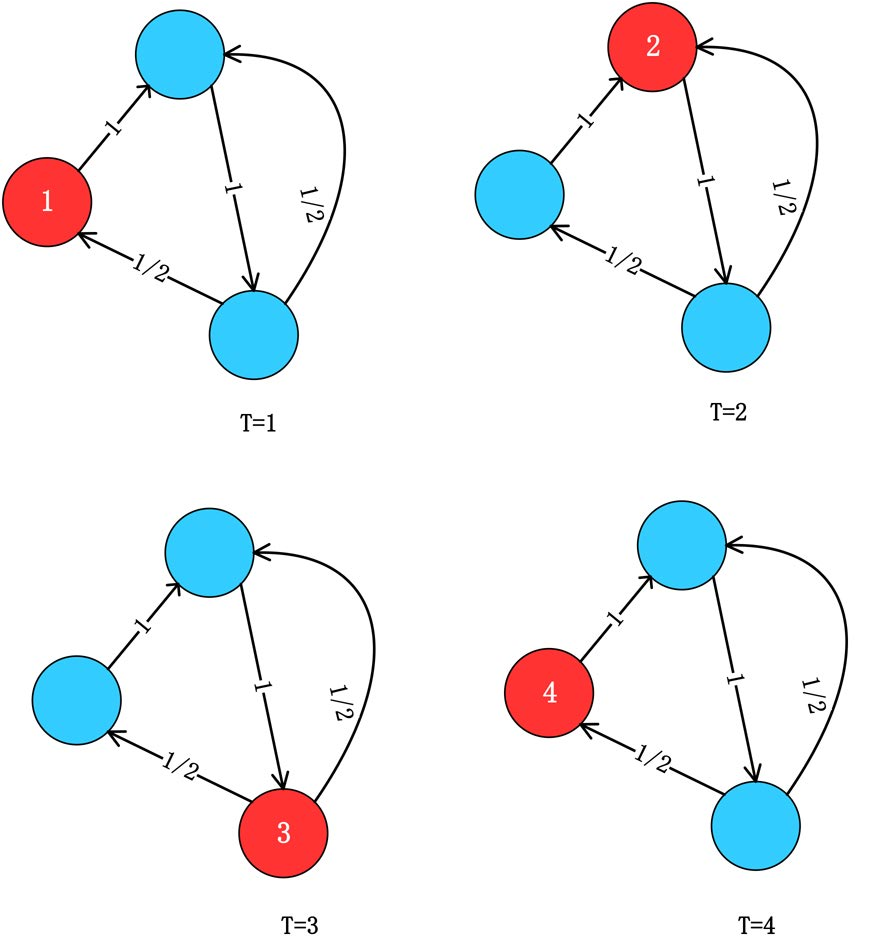
\includegraphics[width = 0.6\textwidth]{rw}
\caption[fig2]{随机游走的实例}
\end{figure}


基于随机游走的一类方法在通路网络扩展和通路中潜在的关联关系的预测应用方面具有重要的价值。所谓的随机游走就是在规则的点阵上进行无规律行走的模型,该模型的每个步骤,从一个位置跳转到另一相邻位置,位置变化形成的一个序列如图\ref{fig2}所示,图中红色节点表示当前时刻点所在的位置。一维的随机游走可以看成马尔科夫链,其状态空间和整数T有关系,并且状态的转移概率(从状态T 转移到状态J 的概率)由式\ref{eq:1}给出
\begin{equation}\label{eq:1}
	P_{T+1,T} = 1-P_{T,T-1}
\end{equation}

基于随机游走概念提出的一系列方法被广泛应用在生物网络扩展和生物网络中潜在的链接预测领域,例如药物的重定位领域。本人在[]中系统的总结了基于网络的药物重定位方法,这些方法对于药物-疾病关系,疾病-通路关系的发现具有重要的意义,这些方法也能很好的迁移到生物通路网络的扩展方面。例如Chipman\cite{chipman2009predicting}等人生物网络上使用了随机游走算法,该方法捕获了生物网络的全局信息,预测出和已知通路相关的部分基因。Macropol\cite{Macropol}提出了一种自启动的随机游走算法,在蛋白质网络上检测到了相关的功能模块(蛋白质通路)。Liu\cite{liu2010link}提出了一种本地随机游走算法,该算法以随机游走算法为基础,实现了在规模的复杂网络中的关联关系的预测,以此来实现生物通路的扩展。该方法具有以较低的复杂度得到高精度的预测结果和扩展结果等特点。


国内学者也对生物通路网络的扩展进行深入的研究。王夏\cite{王夏2009大肠杆菌}等利用马尔科夫聚类的方法在对蛋白质网络进行了综合分析,借助模块分析的方法,预测了蛋白质网络中的相关功能模块,作者整合模块之间的作用关系、GO数据库注释信息、KEGG\cite{kanehisa2008kegg}数据库中的代谢通路数据,提出了一种既能扩展通路网络,又能进行致病性和细胞进程研究的方法,对于生物通路的研究具有十分重要的作用和意义。

李寅珠\cite{李寅珠2012基于蛋白质相互作用网络的代谢}等提出了利用蛋白质相互作用信息来预测扩展生物通路网络的方法。作者在使用蛋白相互作用关系构建的网络上,考虑到蛋白质网络中的一阶、二阶特性,使用聚类分析算法进行了蛋白质网络的功能划分,使得同一个生物通路网络中的蛋白均出现在同一个蛋白质功能模块,以此来发现与通路网络相关的新的蛋白。

郑伟\cite{郑伟2010一种基于随机游走模型的多标签分类算法}等人提出了一种多标签游走算法,即基于随机游走算法的多标签分类算法:首先将含有多标签的复杂网络映射成为多标签随机游走图,然后每当一个未分类(即不具有分类标签)的数据被输入时便建立一个对应的多标签随机游走图序列;最后,再对得到的图序列中每个图建立其相应随机游走模型,得到遍历每个顶点的概率分布,并将其转换为每个标签对应的概率分布,有效地解决了多标签分类的问题。该方法可以通过分类问题解决通路网络扩展问题。

谢\cite{xie2012prioritizing}等人提出了一种叫做Bi-Random Walk的方法,该方法在疾病构成网络上实现了疾病未知链接的预测,可借鉴到生物通路网络的扩展过程中。张巧生\cite{zhang2016network}提出了一种基于网络的生物通络扩展方法,该方法避免了已有的通路分析方法的局限性,实验结果表明该方法具有较强的可靠性和预测精度。

\section{生物通路网络的可视化技术国内外研究现状}[Current research situation version]

随着对生物信息研究的继续,对于通路可视化需求日益增长。在传统的情况下,生物通路网络一般是由生物学专家来绘制,数据库中展示的生物通路图也是静态的不可以编辑的。这种方式很耗时耗力,当发现一个通路中有新的信息时候,更新生物通路十分耗时。针对这些问题大量的可视化工具被开发出来,以IPA为代表的大量通路分析和可视化软件被开发出来,极大的便利了研究者的对生物通路网络图的深入研究,大大节省了研究者的时间和精力。目前主流的通路可视化平台如表\ref{table2}所示

\begin{table}[htbp]
  \centering
	\caption[table2]{当前主流的通路可视化工具}
\vspace{0.5em}\wuhao
\begin{tabularx}{1.0\textwidth}{lX}
\toprule[1.5pt]
名称 & 网址 \\
\midrule[1pt]
Ingenuity Pathway Analysis(IPA)	& www.ingenuity.com\\
GeneGo/MetaCore 	& www.genego.com\\
Pathway Studio 	& www.ariadnegenomics.com\\
GenMAPP	       & www.genmapp.com\\
WikiPathways & www. wikipathways.org\\
Pathway Painter	 & www.pathway.painter.gsa-online.de/)\\
cPath	& www.cbio.mskcc.org/cpath\\
GeneGo/MetaCore 	& www.genego.com\\
Pathway Studio 	& www.ariadnegenomics.com\\
GenMAPP	& www.genmapp.com\\
BioCyc	& www.biocyc.org\\
Pubgene	& www.pubgene.org\\
PANTHER	& www.pantherdb.org\\
WebGestalt	& www.genmapp.com\\

\bottomrule[1.5pt]
\end{tabularx}
\end{table}

当前比较主流的生物通路展示方式多基于JavaScript的可视化技术,因为互联网技术的日益发展,传统的桌面端展示方式不适合人们对信息和数据快速获取和分享的需求,而JavaScript为代表的网页端开发语言,可以实现可视化系统的线上部署访问,用户无下载软件带来时间成本,同时也省去了部分软件在不同的操作系统,不同的架构下的部署使用的繁琐步骤,因此该基于JavaScript的可视化技术越来越受到开发者用户的欢迎,常用可视化库有D3.js, cytoscape.js等。


Cytoscape\cite{}是一款受到用户喜欢的通路网络可视化软件,该软件提供了强大而丰富网络可视化和分析功能,并且实现了跨平台,该软件的研发团队为适应广大的用户的需要开发了Cytoscape.js,也是就是该软件的核心JavaScript库,该库包含了网络布局调整,网络交互、网络下载、数据下载等众多功能,用户基于此库结合自己的需要开发相关的控件、插件、布局配置等,本文第四章所开发的可视化系统也基于该库。


D3.js\cite{}是一款基于数据驱动的前端JavaScript库,该软件库提供了标准的接口封装,用户可以根据自己的需求定制开发自己所需的前端控件, 为用户个性化需求提供了极大的便利。相对于cytoscape 该软件库更加灵活,但是与之带来不便之处是使用该库进行开发工作量比较大,对于系统中具体的实现细节,需要开发者自己去处理,因此对于不熟悉前端技术的开发人员该技术具有较高的门槛。

JavaScript技术为通路可视化提供了极大的便利,同时与生物通路相关数据格式协议,也极大的方便了开发者进行可视化系统的搭建。SBGN\cite{}(系统生物学图形表示法)提供了生物化学和细胞过程可视化表征的一个标准。该标准为生物通路数据提供了同一数据格式,通路数据只需按照这个标准进行存储, 在多个平台和系统下都能进行美观的展示,免去了不同数据展示库在数据格式变化情况下引起的问题,同时基于此标准开发出来的工具可以方便更多用户和研究者使用。

\begin{table}[htbp]
  \centering
	\caption[table2]{基于SBGN标准通路网络可视化工具}
\vspace{0.5em}\wuhao
\begin{tabularx}{1.0\textwidth}{lX}
\toprule[1.5pt]
软件名称 & 网址 \\
\midrule[1pt]
Arcadia	 &  http://arcadiapathways.sourceforge.net/\\
Beacon Pathway Editor	 & https://bioinformatics.cs.vt.edu/beacon/\\
BIOCHAM	 & http://contraintes.inria.fr/biocham/\\
Biographer	 & http://biographer.biologie.hu-berlin.de/\\
BioUML	& http://www.biouml.org/\\
CellDesigner & http://www.celldesigner.org/\\
COPASI	& http://copasi.org/\\
CySBGN	 & https://www.ebi.ac.uk/saezrodriguez/cno/cysbgn/\\
Dunnart	 & http://users.monash.edu/~mwybrow/dunnart/\\
EscherConverter		& https://escher.readthedocs.io/en/latest/escherconverter.html\\
iPathways	 & http://www.ipathways.org/\\
JWS Online	& https://jjj.bio.vu.nl/\\
Mimoza	 & http://mimoza.bordeaux.inria.fr/\\
Newt Editor	& http://newteditor.org/\\
PathVisio	& http://www.pathvisio.org/plugin/sbgn-plugin/\\
PathwayLab	& http://www.innetics.com/\\
SBGN-ED	  & https://immersive-analytics.infotech.monash.edu/vanted/addons/sbgn-ed \\
SBML Layout Viewer	 & http://sysbioapps.dyndns.org/Layout/\\
SBMM assistant	 & http://www.sbmm.uma.es/SPA/\\
yEd Graph Editor	& https://www.yworks.com/products/yed\\

\bottomrule[1.5pt]
\end{tabularx}
\end{table}

国内在生物通路网络的可视化方面也有诸多进展。竺涌楠\cite{}等人设计并实现了一套基于html5 的通路展示系统;胡言石\cite{}等人实现了一种与帕金森相关的生化通路和蛋白质互作网络的可视化系统;黄益灵\cite{}等人实现了一个名为PBSK 的浏览器,该浏览器可以实现四种XML格式的生物通路数据的展示。

\section{主要研究内容}
本课题主要研究的内容是生物通路网络的扩展算法的研究和生物通路网络可视化平台的设计与实现。本课题兼顾到在算法方面的创新性和在平台实现的实用性。

生物通路是细胞中分子间的一系列活动,导致细胞内某种产物或变化。一些通路网络会引起新的分子的组装比如脂肪和蛋白质的生成。生物通络可以控制基因的打开,或者刺激细胞的移动。由于复杂疾病往往和生物通路之间具有密切的关系,与生物通路相关联的多种的基因、蛋白等对于疾病的发病机制具有重要的影响。随着高通量技术的发展,基因、蛋白、代谢等组学数据日益积累,结合这些丰富的生物数据进行生物通路的扩展是一项重要研究手段,对于发掘生物通路潜在的功能,在疾病发病机制研究、临床治疗水平的改善、药物研究等领域具有重要的作用。

目前,有关通路网络的扩展算法主要集中在生物通路网络中链接的预测和生物通路网络的聚类分析,模块发现。这些方法没有很好的利用生物通路网络的拓扑结构关系及网络的自身特点,部分算法时间复杂度过大,计算时需要的软硬件资源过多。因此,提高算法的性能,改善生物通路网络的扩展效果的迫在眉睫。就通路网络可视化技术而言,部分生物通路网路展示软件,属于商用软件的范畴,使用的资金费用过高,部分开源的软件项目,功能又过于零散,因此急需一款较为综合的通路网络可视化和分析软件。因此,本研究从生物网络的特点出发,旨在提出一种高效的快速的生物网络扩展算法,同时将开发一个生物通路网络的可视化展示系统与生物通路网络扩展算法相互结合,便于用户的使用,将算法创新与工程实践相融合。

本文各章节的内容安排如下:

第二章 生物通路网络分析:本章旨在分析生物通路网络的拓扑结构,分析重要网络参数,为第三章算法设计做铺垫,同时为第四章系统中的网络分析部分做准备。

第三章 设计与实现融合生物通路网络特点的扩展算法,在算法的时间性能、扩展质量等方面与已有算法进行对比

第四章 生物通路网络可视化系统。详细的介绍可视化系统的架构、设计理念、开发技术等。


\chapter{生物通路的构建和分析方法研究}
\section{引言}
随着生物通路数据的积累和相关数据库的日益完备,生物通路分析已成为研究的重点。传统的生物通路分析技术没有考虑到通路中基因之间的相互作用对整个通路的影响,因此其分析效果和分析能力有限。随着对复杂疾病的研究日益深入,研究者发现复杂疾病往往是和多种基因相关的,因此使用网络的方法对复杂疾病进行研究成为了当前通路研究的主流。根据美国国家图书馆的统计\footnote{website},研究生物网络的文献数目呈现出爆发式的增长趋势,对生物通络网络研究文献也在逐年上升。

生物通路网络是复杂网络中的一种,对于复杂网络的分析的方法可以迁移到对于生物通路网络分析当中。生物通路网络中的作用关系是动态变化的,因此反应在网络中,通路网络节点之间的作用会随着时间和外部条件的不同而变化,因此网络具有一种动态的特征,这种特点和复杂网络的特征是相符合的,因此复杂网络的分析方法在生物通路网络同样适用。生物通路网络的拓扑属性、 网络特性、重要网络参数等可以作为通路网络进行扩展的依据。

本章中我们讨论了生物通路网络的构建方法,基于建立的生物通路网络进行了网络拓扑结构、网络参数、中心性等分析,进而为生物通路网络扩展算法的研究奠定基础。

\section{数据的选取与分析}
生物通路网络的分析方法借鉴了一般网络的分析和扩展方法,将生物通路网络背景建立在已有的生物网络中,借助对这些网络分析,以此达到扩展通路网络的目的。因此,选择合适的通路数据库和网络结构数据库是十分重要的,在本文中,我们适用包含大量可靠的PPI关系的生物网络HumanNet\cite{}作为基础网络,同时选取KEGG\cite{}数据库作为通路数据的来源, 同时作为验证数据使用BRCA作为数据来源,以下我们将这几个数据库进行详细介绍。

KEGG\cite{}Kyoto Encyclopedia of Genes and Genomes)是一套日本于1995年制定的人类基因组计划,此为关于基因组、酶促途径以及生物化学物质的在线数据库。其途径数据库PATHWAY之中记录的是细胞之中的分子相互作用网络以及具体生物所特有的变化形式。KEGG\cite{}提供了一个分类体系,在同一条通路上的有相似的或者相同的功能蛋白质会被归为一组,在本文中KEGG中数据会作为通路扩展的种子节点。

HumanNet\cite{}是韩国延世大学和奥斯汀德克萨斯大学的联合研究成果。HumanNet\cite{}整合了21种不同物种的组学数据,根据这些生物数据与已知的人类基因之间的功能作用强弱,这些数据被赋予不同的权重,并通过改进的贝叶斯方法构建了网络结构,形成了一个概率功能网络。HumanNet\cite{}囊括了18 714个编码基因,25 421对基因间的相互作用,在HumanNet\cite{}中每个节点代表一个编码基因,每一条边代表两基因间的相互作用并被赋予了权重,该权重是一个相关的对数似然得分,表征两基因间相互作用的概率。HumanNet\cite{}为基因的优先选择提供了一个通用的方法,对于一个给定的基因,HumanNet\cite{}会提供一个该基因与其他基因关联的次序,便于挖掘疾病在基因层面的关联关系。HumanNet\cite{}也为研究者提供了用户接口(http://www.functionalnet.org/humannet)以方便研究人员进行相关的研究工作。由于该网络融合了多种类型的信息,并且具有较强的通用性,在这篇文章中我们采用HumanNet\cite{}作为基础网络构建我们的功能网络。

BRCA数据集是从癌症基因组网站TCGA(英文名全称:The Cancer Genome Atlas,网址为http://cancergenome.nih.gov/)下载的数据,该数据由590个样本组成,其中521个是乳腺癌样本,61个样本是符合正态分布的样本。该数据由于数据质量较好,被广泛的应用于癌症通路的识别,药物靶点发现,药物重定位的研究。

\section{网络的构建方法研究}[cons]
\label{cons}
我们选择HumanNet作为基础网络,基因关联网络已经被广泛的应用于理解疾病。HumanNet是一个综合了人类基因的网络,我们在HumanNet上获取基因对之间的相互作用的强度,在HumanNet中基因间的作用强度用一个对数似然分值S表示,S的值是一个大于1 的实数,为了避免由量度引入的误差,我们采用离差标准化将基因间的强度进行归一化由式\ref{eq21}给出
\begin{equation}\label{eq21}
SN=\frac{S( g_{i} \ ,g_{j} \ ) \ -\ S_{min}}{S_{max\ } -\ S_{min}}
\end{equation}

\begin{tabularx}{\textwidth}{@{}l@{\quad}r@{———}X@{}}
式中& $\boldsymbol{SN}$ & 标准化后对数相似分数值;\\
	& $\boldsymbol{S_{max\ }}$ &HumanNet中最大的对数似然分值;\\
	& $\boldsymbol{S_{min\ }}$ &HumanNet中最小的对数似然分值;\\
	 & $\boldsymbol{ g_{i}, g_{j}}$ &HumanNet中的基因;\\
	& $\boldsymbol{S( g_{i} \ ,g_{j} \ )}$ & 标准化之前对数似然分数值;\\
\end{tabularx}\vspace{3.15bp}

\begin{figure}
\centering
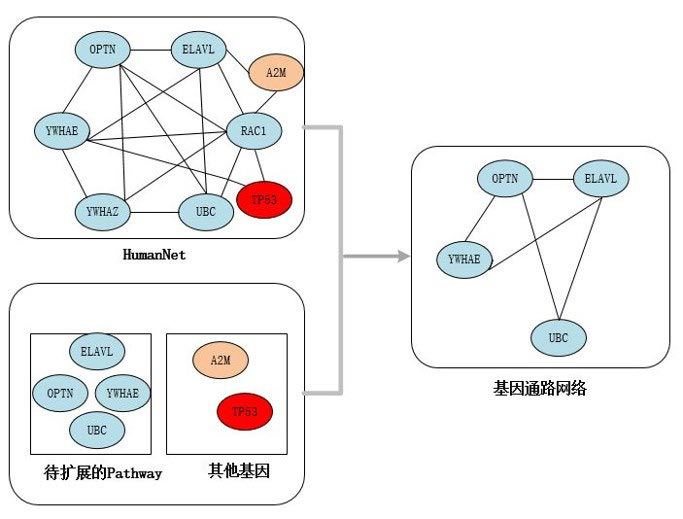
\includegraphics[width = 0.8\textwidth]{pathway_cons}
\caption[fig21]{通路网络的建立过程}
\label{fig21}
\end{figure}
通路网络 是一个带权图G(V, E),其中集合 V是由基因组成的集合。E是边集,E中的每一个元素$e_{ij}=(v_{i}, v_{j})$代表基因之间的相互作用。如果与 $v_{i}$和$v_{j}$对应的基因$g_{i}$和$g_{i}$ 对应的边$< g_{i} ,g_{j}  >$存在于HumanNet中那么就把边 $< v_{i} ,v_{j}  >$加入集合E中(如图\ref{fig21}所示), $w_{ij}$ 是集合W中的一个元素,它代表 $v_{i}$和 $v_{j}$作用的强弱, 被量化如下:
\begin{equation}\label{eq22}
w_{ij} ( v_{i} ,\ v_{j}) =SN( g_{i} ,g_{j})
\end{equation}
\begin{tabularx}{\textwidth}{@{}l@{\quad}r@{———}X@{}}
式中 & $\boldsymbol{ g_{i}, g_{j}}$ &HumanNet中的基因;\\
	& $\boldsymbol{SN( g_{i} ,g_{j})}$ & HumanNet中标准化后对数相似分数值;\\
\end{tabularx}\vspace{3.15bp}
至此,通路网络被建立起来。


\section{ 通路网络的分析方法}
由于本文第三章将探究通路网络的扩展算法,因此对通路网络的分析是进行算法设计的基础。作为复杂网络的一种,生物通路网络
具有复杂网络的共性,同时也有其自身独有的特点。由于复杂网络的理论已经在社交网络分析,蛋白质功能预测、个性广告推荐等领域取得了较好效果,因此这些成熟的复杂网络分析方法也将帮助我们了解生物通路网络的特点,为实现该网络的扩展,生物通路网络的部分特点也将作为网络扩展的部分依据。

复杂网络的分析主要集中在其拓扑结构、 网络参数、 中心性等方面。网络的拓扑结构可以反映网络整体的特征,一些基于网络整体信息的方法如基于信息传播的方法\cite{}都是基于网络的拓扑结构和性质; 网络的参数分析可以反应在度分布、连通域分布、共享邻居分布、最短路径分布等方面,这些网络参数既有基于局部的特点、也有基于全局的特点的。中心性则集中在对网络中节点重要性的衡量上,传统的网络扩展方法大部分基于公共邻居、基于度\cite{}等信息,反应节点在网络中的重要性质时信息过于单一,因此对于中心性的分析将帮助研究更好的衡量和评价节点的重要性。

在本节中我们将介绍通路网络的节点度分布、平均聚类系数分布、拓扑系数、最短路径分布、共享邻居节点分布、邻域连通性分布、介数中心性、紧密中心性等属性。同时结合具体的生物通路网络实例进行简要的分析。

\subsection{度分布}
图结构中与某节点相连接的边的数目为该节点的度,而图中各个的节点度的散布情况就为度分布。度分布是节点度信息在网络中的一个总体描述。一个无向图 ${\displaystyle G=G(V,E)}$ 是指某个节点$ {\displaystyle v_{i_{0}}}$与之相连所有的节点的数目。

\begin{equation}\label{eq22}
	d( v_{i_{0}}) =\sum\limits ^{e_{i,j} \in E\ }_{i=i_{0}} e_{i,j}
\end{equation}
度分布则是对每个非负整数 ${\displaystyle m}$, 度为m的顶点在所有的顶点的比例,可以形式化如下:

\begin{equation}\label{eq23}
{\displaystyle \forall m\in \mathbb {N} ,\,\,P:m\mapsto P(m)={\frac {\operatorname {Card} \{v_{i}\,|\,d(v_{i})=m\}}{n}},}
\end{equation}
其中: Card 为计数函数。其中一个约束条件为$ {\displaystyle \sum _{m\in \mathbb {N} }P(m)=1}$

\subsection{平均聚类系数分布}
平均聚类系数表示一个图形中节点聚集程度的系数。是一个用来衡量网络节点聚类的情况的参数。 其数学定义如下
\begin{equation}\label{eq24}
CC_{v2} =\frac{2n}{_{k( k-1)}}
\end{equation}
\begin{tabularx}{\textwidth}{@{}l@{\quad}r@{———}X@{}}
式中 & $\boldsymbol{k}$ &  表示节点v2的所有相邻的节点的个数,即节点v2的邻居;\\
	& $\boldsymbol{n}$ &   表示节点v2的所有相邻节点之间相互连接的边的个数;\\
	& $\boldsymbol{CC_{v2}}$ &	节点V2的平均聚类系数值 \\
\end{tabularx}\vspace{3.15bp}

\begin{figure}[h]
\centering
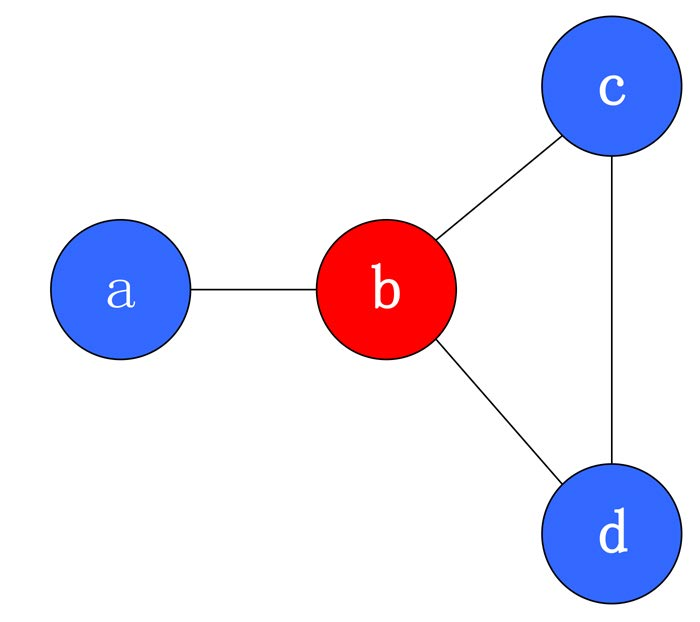
\includegraphics[width = 0.3\textwidth]{fig22}
\caption[fig24]{聚集系数计算的示例图}
\label{fig24}
\end{figure}

聚集系数表示一个图中节点的聚集程度,在实际的网络中,相对高密度的连接点关系具有某种组织结构属性,聚集系数高的连接之间存在关联性的概率大于两点随机建立的连接的概率。整个网络的聚集系数是网络中所有的节点的聚集系数的平均值。图\ref{fig24}给出了一个实例图中节点b 的聚集系数计算实例。与b 相邻的节点个数是3个因此k 的取值是3; 在与b相连的节点中其中相邻的有c和d,因此n的取值是1由计算公式可得 $CC_{b}=1/3$。


\subsection{最短路径分布}
由于生物通路网络被看做图模型来进行研究,因此图上的最短路径求解算法都适用于生物通路网络,常用的最短路径求解算法有Dijkstra\cite{}算法,Bellman-Ford\cite{}算法,Floyd\cite{}算法等。
最短路径分布就是按照给定的算法计算图中两两之间的最短距离,统计最短路径的分布情况,最短路径分布反映出网络宏观上结构特点如小世界性等特点\cite{Article Navigation
Computing topological parameters of biological networks}。

\subsection{邻域连通性分布}
某一个节点的连通性指的是它的邻居节点的个数,某一个节点的邻域连通性指的是该节点对应所有邻居节点的连通性数值的平均值。这里邻域连通性分布指的是对含k个邻居节点的目标节点的邻域连通性值的分布(k=0,1,2……)。如果邻域连通性分布是k的递减函数 ,那么网络高连通的节点更趋于边缘化。若为递增函数,则这些高连通的节点更趋于网络中心。
\subsection{介数中心性}
介数包括节点介数和边介数两个概念。节点介数是指网络中通过该节点所有最短路径的数量与所有路径的数量之间的比例。边介数表示通过该边的所有最短路径的数量和所有路径之间的比值。介数的现实意义是反映了节点(边)在网络中的重要程度和其在整个网络中的控制能力。节点介数中心性定义如下
\begin{equation}\label{eq26}
	C_{b}( b) =\sum\limits _{s\neq b\neq t} \sigma_{st}( b) /\ \sigma_{st}
\end{equation}

\begin{tabularx}{\textwidth}{@{}l@{\quad}r@{———}X@{}}
式中 & $\boldsymbol{s,t,b}$ &  网络中的节点;\\
	& $\boldsymbol{ \sigma_{st}}$ &   表示s到t的最短路径条数;\\
	& $\boldsymbol{\sigma_{st}( n)}$ &	表示通过n的s到t最短路径条数 \\
\end{tabularx}\vspace{3.15bp}
计算中,通常除以一个:(N -1)(N -2)/ 2,其中N表示节点n参与其他节点连接的节点总数(包括n)。
在图\ref{fig25}中 $C_{b}( b) =\sum\limits _{s\neq b\neq t} \sigma_{st}( b) /\ \sigma_{st} =  0.583$

节点的介数中心性反映了该节点对网络中其他节点的控制能力,可以有效的衡量该节点在网络中的核心重要程度。



\begin{figure}[h]
\centering
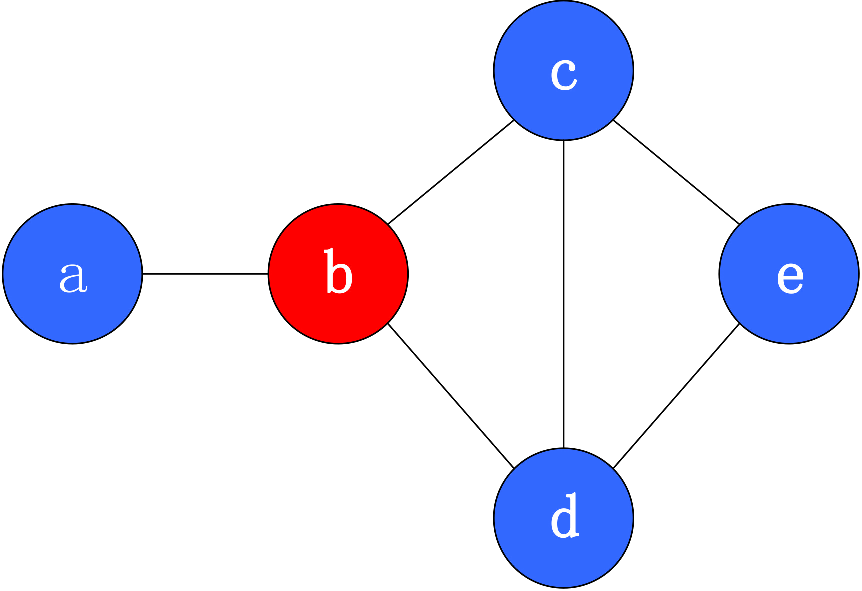
\includegraphics[width = 0.3\textwidth]{toplog}
\caption[fig25]{拓扑系数计算的示例图}
\label{fig25}
\end{figure}

\subsection{拓扑中心性(拓扑系数)}
拓扑系数反映的是网络中的节点具有共享邻居的趋势。数学形式定义如下
\begin{equation}\label{eq25}
	T_{n} =\ \frac{avg( J( n,m))}{k_{n}}
\end{equation}
\begin{tabularx}{\textwidth}{@{}l@{\quad}r@{———}X@{}}
式中 & $\boldsymbol{k_{n}}$ &  表示节点n的所有相邻的节点的个数,即节点v2的邻居;\\
	& $\boldsymbol{ J( n,m)}$ &   表示节点n和m  之间共享的邻居的个数;\\
\end{tabularx}\vspace{3.15bp}
需要说明的一点是如果n没有邻居节点,那么此时n的拓扑系数为0,拓扑系数反映了一个节点和其他节点之间共享邻居的一种趋势。以图\ref{fig25}为例计算节点b的拓扑系数:由于图 中J(b,c)= J(b,d)= J(b,e)= 2故 $T_{b}=2/3$。


\subsection{紧密中心性}
紧密中心性是衡量信息从给定节点到网络中其他可到达节点的传播速度的一个度量标准,更直观地讲,它反映的是某节点到达其他节点的难易程度。节点n的紧密中心性被定义为该节点到其他所有节点的最短路径长度平均值的倒数。定义孤立节点的紧密中心性值为0。

\begin{equation}\label{eq27}
	Cc( b) =1/avg( L( b,\ m))
\end{equation}

\begin{tabularx}{\textwidth}{@{}l@{\quad}r@{———}X@{}}
式中 & $\boldsymbol{L(n, m)}$ &  表示n、m节点对之间的最短路径长度;\\
\end{tabularx}\vspace{3.15bp}
以图\ref{fig25}为例,计算图中的b的紧密中心性的过程为$Cc(b) = 1/ ( (L(b, a) + L(b, c) + L(b, d) + L(b, e)) / 4) = 4/ (1 + 1 + 1 + 2) = 4/5= 0.8$

\section{生物通路网络分析结果}
在本节中,我们筛选了290个KEGG\cite{}数据库中和人类相关的生物通路,使用\ref{cons}节的网络构建方法创建了290个生物网络,以这些网络为基础,我们使用上一章的网络分析方法,对这些网络进行了详细的分析,结果如下
\subsection{度分析结果}
图\ref{fig26}是290个与人类相关的通路网络的度的平均值统计,从图中可以看出,大部分网络的度的平均值集中在10以下,因此网络呈现出一定的稀疏性,也就说明大多数的通路网络中 众多节点只和很少节点连接,而有极少的节点与非常多的节点连接。间接可以反映出网络中部分节点起到“关键”的作用。在后期扩展算法设计中这些在网络中具有“关键”作用的节点应该成为通路网络被扩展的对象。同时由同种橙色的虚线可以看出,随着度的增加,通路网络的数量越来越少,并且这种减少的趋势是符合幂率分布的特点,这种特点显示出网络存在无尺度的特性,

\begin{figure}[h]
\centering
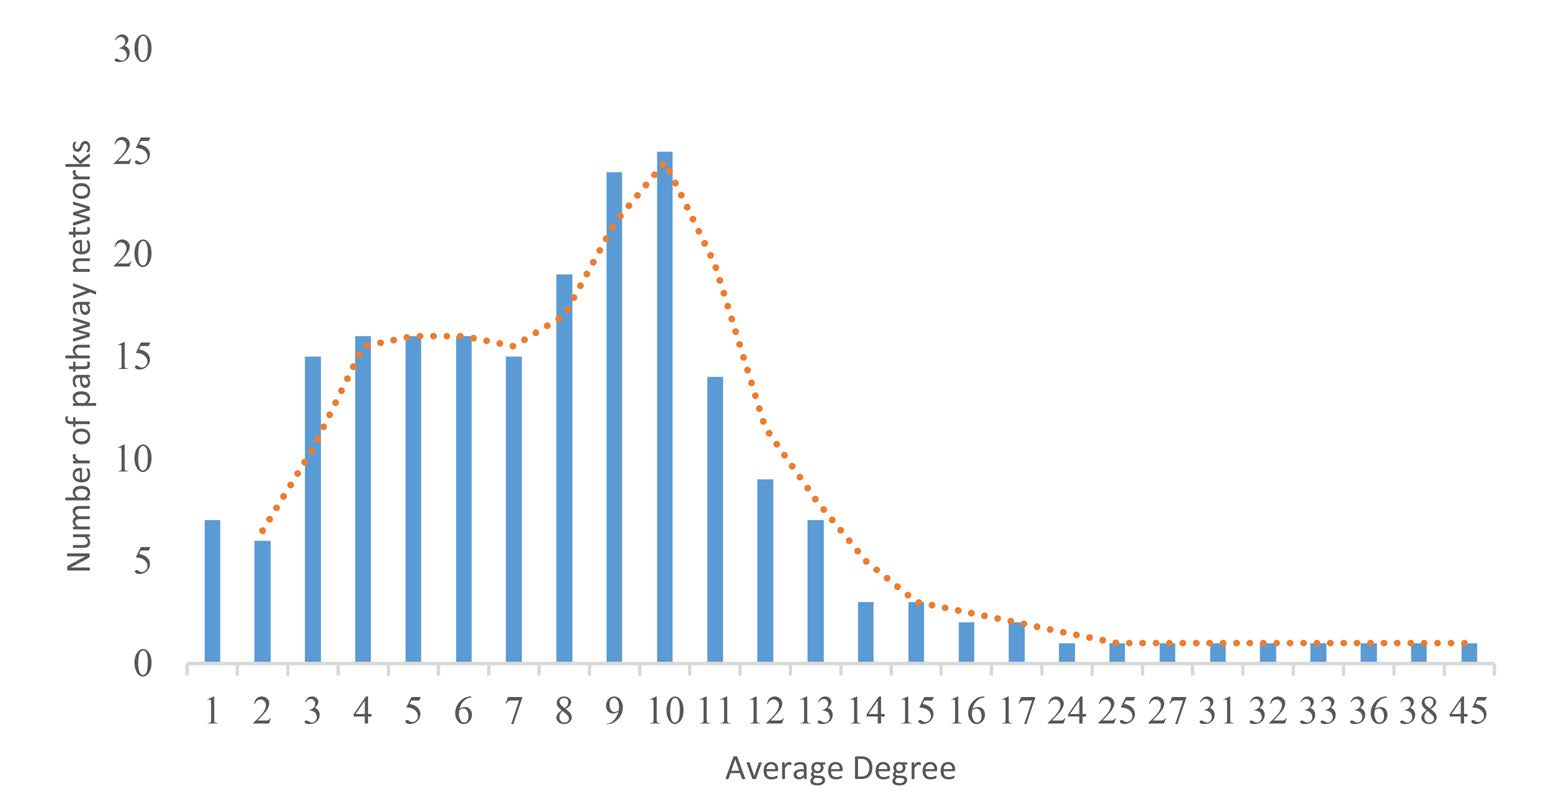
\includegraphics[width = 0.95\textwidth]{degree_dis}
\caption[fig26]{生物通路网络度的平均值统计}
\label{fig26}
\end{figure}

\subsection{最短路径分析结果}
图\ref{fig27}是290个与人类相关的通路网络的最短路径平均值统计, 从图中可以看出绝大数的网络(约占80\%的生物通路网络)的最短路径的平均值是2-3,说明这些生物通路网络具有小世界网络\cite{}的特点。在这种图中大部分的结点不与彼此邻接,但大部分结点可以从任一其他点经少数几步就可到达 ,平均最短路径长度可以反映这个网络的全局特征,也间接说明在通路网络中扩展其邻居、二度邻居节点的可能性要比扩展其他节点的可能性更大。

\begin{figure}[h]
\centering
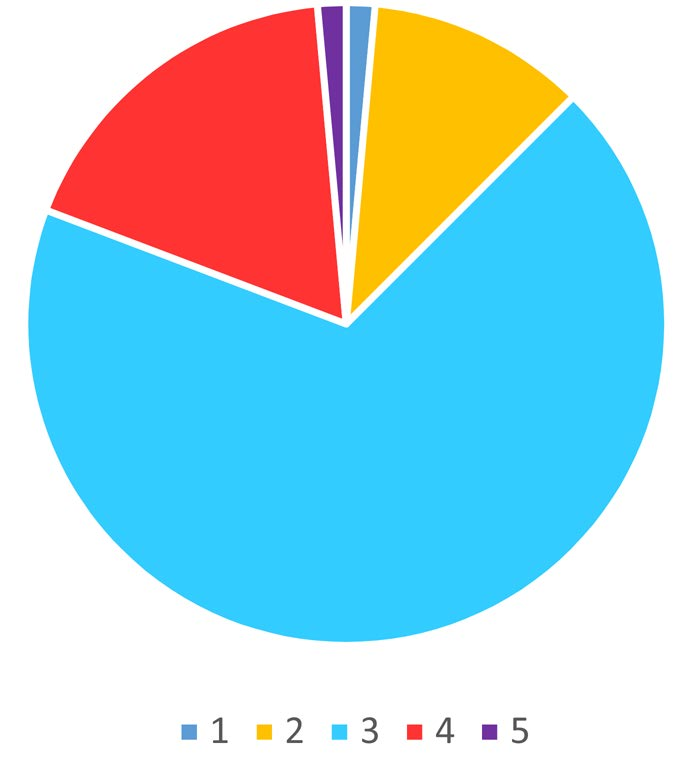
\includegraphics[width = 0.35\textwidth]{pie}
\caption[fig27]{生物通路最短路径的平均值统计}
\label{fig27}
\end{figure}

\subsection{平均聚集系数分析结果}

由上一节的分析结果可知生物通路网络具有小世界网络的特点,反映小世界网络特点的主要参数除了平均最短路径长度,还有聚集系数。由上一节我们可知小世界网络里大部分结点可以从任一其他点经少数几步就可到达,这个参数反映了节点邻居的邻居和该节点的相关程度,因此在通路网络扩展过程中聚集系数是十分重要的一个参数。同时图\ref{fig28}统计结果显示,290张通路网络的平均聚集系数符合正态分布,大部分的通路网络平均系数在0.5左右,因此我们可以通过设置聚集系数的阈值大小来控制通路网络的扩展规模。
\begin{figure}[h]
\centering
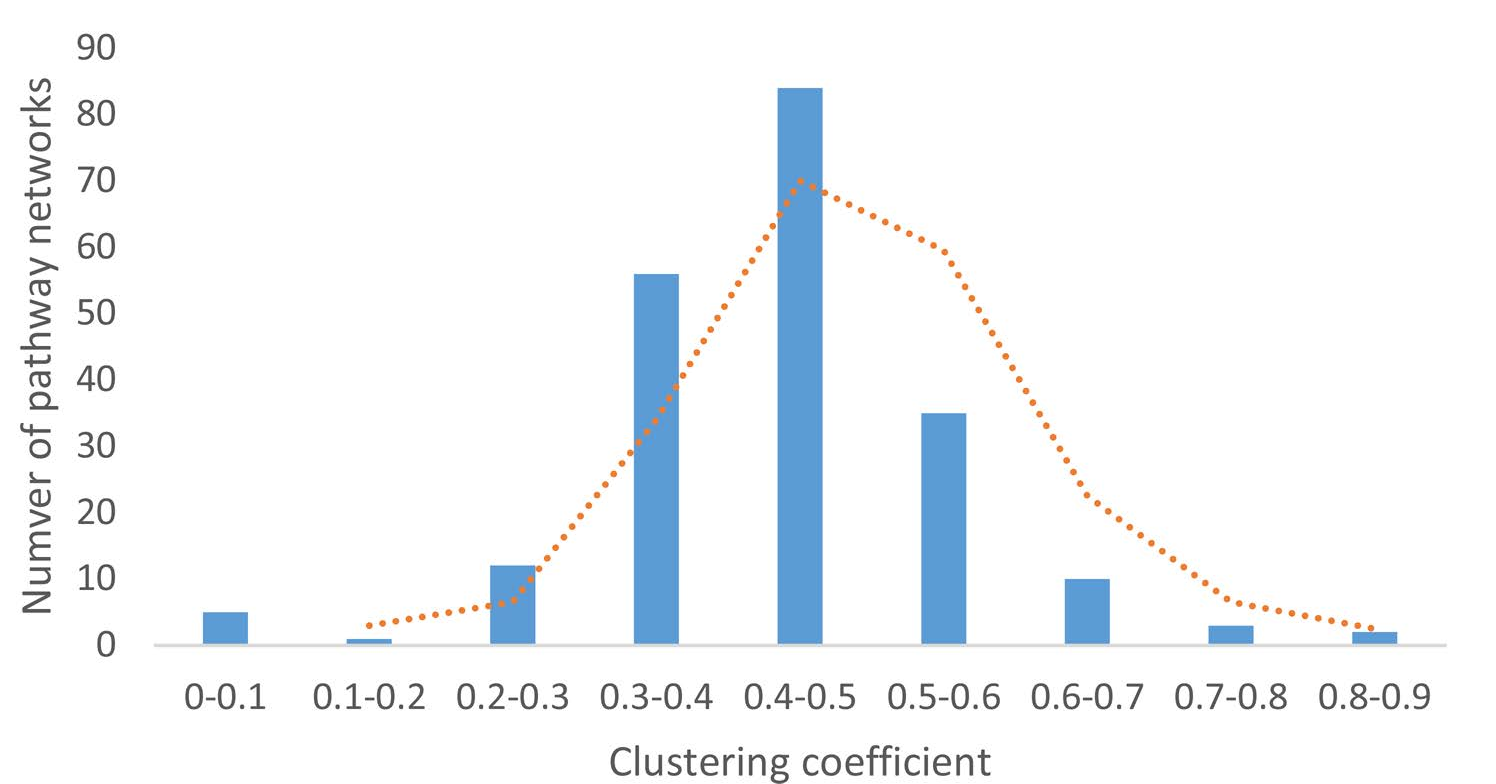
\includegraphics[width = 0.95\textwidth]{cc}
\caption[fig28]{平均聚集系数分析结果}
\label{fig28}
\end{figure}

\subsection{中心性}
图\ref{fig29}是290个与人类相关的通路网络的中心性分析的结果,我们分析了介数中心性(Betweeness Centrality记为BC)、紧密中心性(Closeness Centrality记为CC)、拓扑中心性(Topological Centrality记为TC)。介数中心性强调的是节点的控制能力,紧密中心性强调节点在网络中的重要性、拓扑中心性刻画了网络拓扑结构上的重要性。

从图\ref{fig29}可以看出,大部分生物通路网络的介数中心性都比较小,并且这些通路网络的介数中心性分布集中且值都比较小,说明大部分网络中节点对其他的节点控制能力都比较弱,符合上文中所提到的这些网络具有小世界属性和无尺度网络的属性。介数中心性的统计结果显示有很多异常点,说明有部分网络中节点控制能力十分强,说明这些网络在其结构上有特异性。在通路网络扩展算法的设计中,需要考虑到大部分网络的共同的特点,其特异性可能造成通路网络扩展结果的随意性,因此在设计生物通路网络扩展算法的设计当中介数中心性不是一个很好的参数来评估网络节点的重要性。

从图\ref{fig29}可以看出,生物通路网络的紧密中心性分布均匀,绝大数点的紧密中心性都在0.3以下,说明大部分的生物通路网络节点不是十分密集,只有少数的节点在网络中能迅速的到达其他节点,在生物通路网络的扩展算法设计过程中需要考虑少数的具有重要性的节点。同时从不多的几个异常值可以发现,有部分网络的节点到达其他节点的能力极强,考虑这部分网络的扩展策略时可能需要考虑到这些网络密集性特点。

从图\ref{fig29}可以看出,生物通路网络的拓扑中心性分布均匀,拓扑中心性的统计结果中异常值很少,说明大部分的生物通路网络在拓扑结构上是类似的,在设计通路网络的扩展算法时,这些网络类似的拓扑结构特点可以作为生物网络扩展依据。

\begin{figure}[h]
\centering
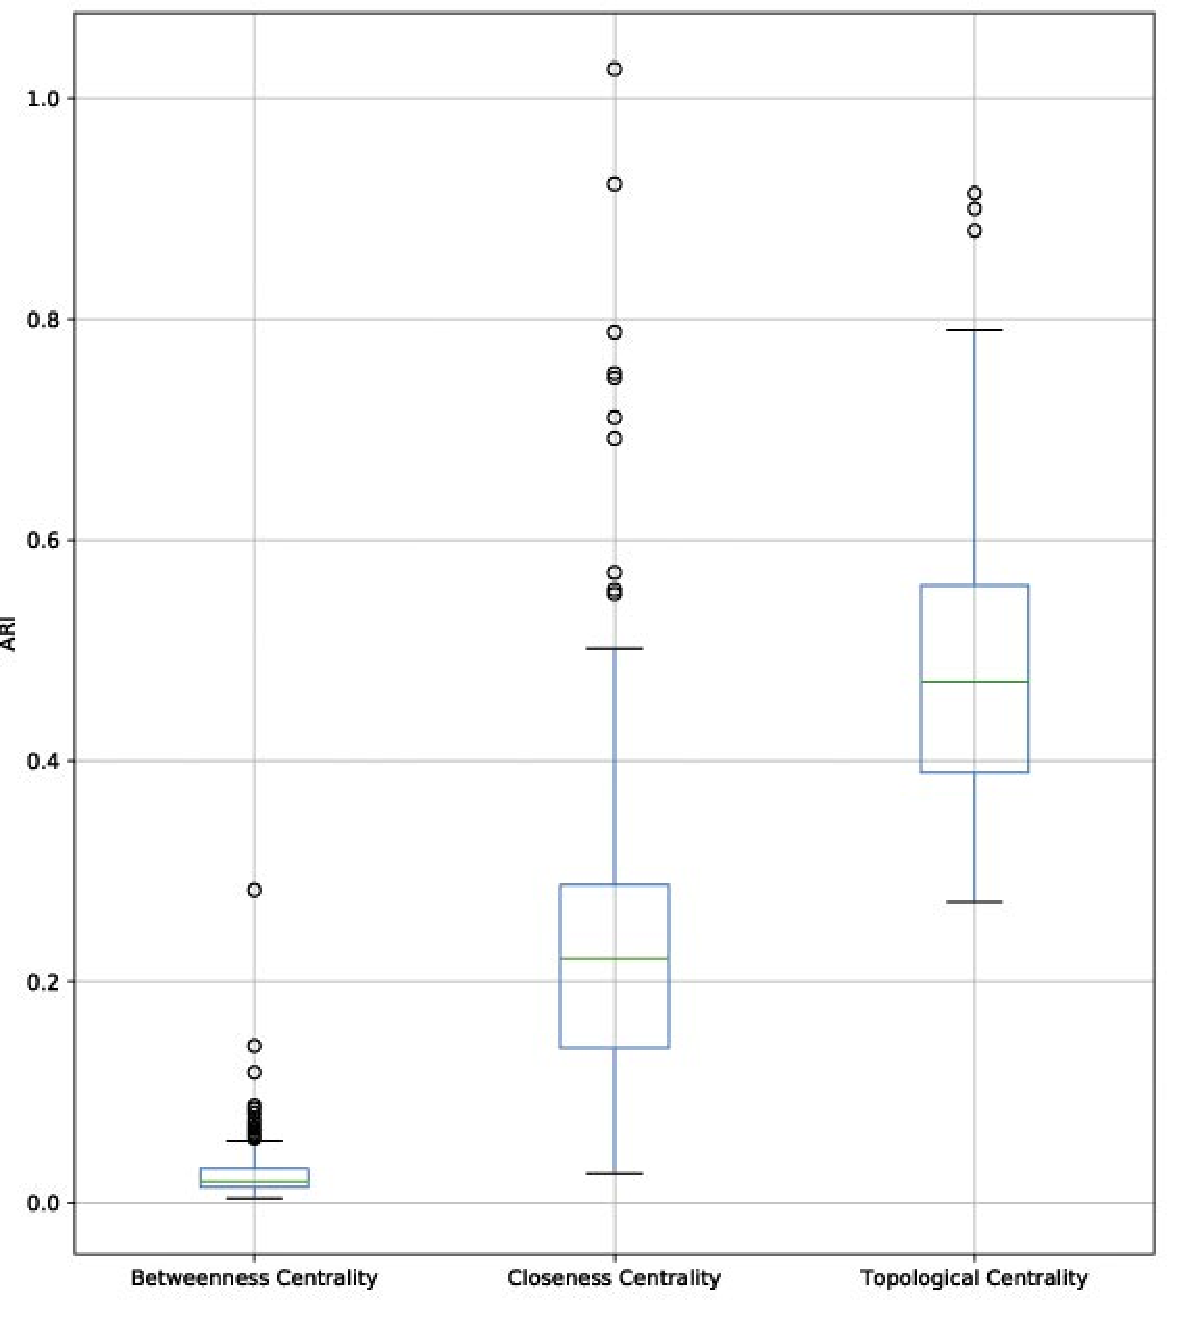
\includegraphics[width = 0.6\textwidth]{center_summary}
\caption[fig29]{生物通路网络中心性分析结果}
\label{fig29}
\end{figure}

\section{本章小结}

在本章中我们介绍了本文中使用的生物通路网络数据,同时提出了生物通路网络的构建方法。我们从KEGG数据库中选取290个与人类相关的生物通路数据,建立了其生物通路网络。为研究生物通路网络的特点,为一章生物通路网络的扩展算法奠定基础。我们介绍了通路网络的节点度分布、平均聚类系数分布、拓扑系数、最短路径分布、共享邻居节点分布、邻域连通性分布、介数中心性、紧密中心性等分析方法,并在290张生物通路网络上使用了这些分析方法,做了简单的统计。

经过我们的分析我们建立的290张生物通路网络具有小世界网络的特点即:图中大部分的结点不与彼此邻接,但大部分结点可以从任一其他点经少数几步就可到达。同时由最短路径分析我们得知大部分生物通络网络最短路径的平均值是2-3,说明在生物通路网络扩展算法的实际中应该着重的考虑节点的邻居、二度邻居的重要性。同时,通路网络的聚集系数分析显示,这些网络中的聚集系数可以作为网络扩展的重要依据。

\chapter{生物通路网络扩展算法研究}
\section{引言}
复杂疾病可能与多种基因、蛋白质和生物通路的影响有关\cite{大师兄[1]}。结合多种的高通量数据生物通路和复杂疾病之间的关联研究已经成为了研究者的首选。生物通路往往和多个基因关联,通路的活动对于复杂疾病具有重要影响。因此,深入的研究生物通路与复杂疾病之间的关联,有助于揭示复杂疾病的发病机制,对于疾病治疗方法研究、针对特定疾病的药物开发、药物重定位等领域具有重大意义。

第一代的生物通路分析技术是以ORA\cite{goeman2007analyzing}方法为代表。该方法的使用特定阈值和标准创建输入列表。然后输入一个基因的列表,使得每个列表里的基因都是生物通路的一部分,接下来对于每一个通路在输入基因列表时进行相关的测试得到最后和输入基因最为显著相关的通路,然后这种方法具有明显的缺陷,由于使用的信息有限,该技术的实验效果不佳。为了改善实验的效果,更为先进的生物通路分析方法被提出,其中以FCS\cite{lee2011prioritizing}为典型的代表。FCS克服了ORA缺点,并实现了在从分子测量角度寻找到生物通路上的显著基因。FCS用一个统一的分数将各种不同的统计分析方法得到的结果结合了起来。OFA 和FCS方法仅仅考虑了生物通路上基因的数量和基因表达信息来确定关键的生物通路。FCS\cite{lee2011prioritizing}考虑到了
通路间数量和基因表达上的信息,与ORA相比其实验有明显的提升,但是由于通络中的基因是相互关联的,这些基因组成的生物通路网络的拓扑结构、作用关系等和复杂疾病具有关联,因此使用基于网络方法的生物通路分析技术成为了当前研究的热点。

生物通路网络扩展算法是重要的生物通路分析方法,生物通路扩展的步骤是:在全局网络上创建生物通路网络并将其作为种子网络,使用特定扩展策略和方法将全局网络中与种子节点紧密相关的节点纳入到给定的生物通路网络中。经过扩展后纳入通路网络的这些节点与某些复杂疾病之间具有紧密关联。

本章中我们将介绍几种具有代表性的生物通路网络扩展算法并结合上一章通路网络分析方法提出了一种基于搜索策略的生物通路网络扩展算法,并且以HumanNet为全局网络的进行了通路网络的扩展实验,评估了这些方法的扩展效果和算法运行时间。

\section{基于链接预测的通路网络扩展算法}
链接预测是指将生物通路网络作为通路种子网络,在全局网络中预测与通路种子网络中节点相关的链接,将这些链接中的节点纳入扩展后的生物通路网络。形式化如下:将生物通路网路看成一个无向图G(V,E), 在这里V代表节点的集合,E代表链接(边)的集合,图G不允许存在环。用U表示全集,其中包含$\frac{|V|*|V-1|}{2}$个可能的链接,U中的一部分链接存在于待扩展的全局网络里。待预测链接集合为U-E。

链接预测方法最简单的框架是基于相似性的算法,对于$\forall x,y\in V$ 分配一个分数$S_{xy}$。记$e(x,y)$为E中的元素,对$\forall x,y\in V$ 且$e(x,y) \notin E$根据分配的分数从高到低进行排序,通过选择阈值将得分较高的链接纳入到通路网络中。尽管基于相似度的算法比较简单但仍然是当前研究的一个热点。但实际上,节点的相似度的度量仍然是一个挑战。很多情况下,相似性度量是基于已有经验选择的。相似性度量有可能在一些网络中运行良好,在另一些网络可能效果不好\cite{Link prediction approach to collaborative filtering, in: Proceedings}。

节点相似性可以通过使用节点的基本属性来定义, 如果它们有许多共同的特点。但是,节点的属性通常是隐藏的,因此我们将重点放在基于网络结构的相似性。结构相似性可以按照多种方式分类:局部相似性和全局相似性,参数相关的相似性和参数无关的相似性,路径依赖和路径无关的相似性。相似指数也可分为结构等价和规则等价。前者包含一个潜在的假设,即链接本身表示两个端点之间的相似性。后者假定如果两个节点的相邻节点相似,则它们是相似的。本节将介绍三种基于公共邻居个数的相似性度量。

对于一个节点x,令$F(x)$是x的邻居节点的个数,从常识角度讲,对于节点x和节点y如果二者很相似,那么其公共邻居很多,其最简单的度量是衡量二者的重叠的公共邻居个数,即:

\begin{equation}
	S_{xy} = |F(x) \cap F(y)|
	\label{eq31}
\end{equation}

在这里$|F(x)$ $\cap$ $F(y)|$是集合  $F(x)$ $\cap$ $F(y)$的基数。我们记$A$为图的邻接矩阵

\begin{equation}
  A_{xy}=\left\{
 \begin{array}{rcl}
 0      &      & {e(x,y) \in E}\\
 1      &      & {e(x,y) \notin E}\\
 \end{array} \right. 
\end{equation}

显然,在式\ref{eq31}中$S_{xy}=(A^2)_{xy}$,同时我们注意到$(A^2)_{xy}$是对于图G中有连接两个点x,y之间长度为2的不同的路径个数。通常情况下$S_{xy}$会按照一定的方式做规范化。以下的两个度量是使用不同的规范化方法得到的相似性度量。

Salton系数,被定义如下:
\begin{equation}
S_{xy} =\frac{F( x) \cap F( y)}{\sqrt{k_{x\ \ } *\ \ \ k_{y}}}
\end{equation}
在这里$k_{x}$是节点的度,Salton指数在其他文献中也被称为余弦相似度。

Jaccard系数,被定义如下:
\begin{equation}
S_{xy} =\frac{F( x) \cap F( y)}{F( x) \cup F( y)}
\end{equation}
这个系数很早之前被提出,但被广泛的使用。

\section{基于网络传播的通路网络扩展算法}
除了基于链接预测的方法,基于网络传播的算法在生物通路网络扩展的方面具有较为广泛的应用。这一类算法的主要思想是为通路网络的节点分配一个初始信息值,然后使用一定的传播策略将这些信息值向全局网络中传播,待传播过程收敛,计算未在通路网络中的节点和通络网络节点的关联程度,将关联程度较高的节点纳入到生物通路网络中,本节我们将介绍一个基于网络传播的算法,并将其应用到生物通路网络的扩展。

Martinez\cite{}提出了一种基于异质网络传播的方法,所谓传播是指为在网络的已知信息节点n分配一个值v。当算法开始工作时,这个信息按照一定传播规则到达目标网络,直到所有节点的信息趋于稳定,算法停止。传统的基于传播的方法如\cite{}其缺陷在于信息在网络中传播的规则过于单一,因此实验的效果不佳。但Martinez\cite{}考虑到这一点,并加以改进。作者将全局网络分成不同的子网,每个子网代表不同的生物通路网络,作者定义了子网内传播和子网间传播的方法。对于同一个子网(生物通路网络)信息传播按照

\begin{equation}
x_{i+1} =\alpha *M*x_{i} \ +( 1-\alpha ) *x_{0}
\label{eq321}
\end{equation}

其中$\alpha$ 是一个与先验信息有关的参数,M是网路的邻接矩阵, $x_{i}$代表各个节点在第i次迭代时的分配到的值。 对不同的子网而言,定义了一种网络间传播的方式
\begin{equation}
\psi (v) =\frac{\sum ^{x\in neig(v)} \psi (x) \ }{|neig(v) |}
\label{eq322}
\end{equation}

其中:$\psi(v)$代表下一个子网中节点v所分配到的值,neig(v)是节点v的邻居节点的集合。该方法可以将当前子网中的值分配到下一个网络中的节点,下一个子网中信息按照同一子网的传播方式进行传播,直到所有网路中所有的节点的值趋于稳定,以下是该算法工作的示意图如图\ref{fig41}所示:

\begin{figure}[h]
\centering
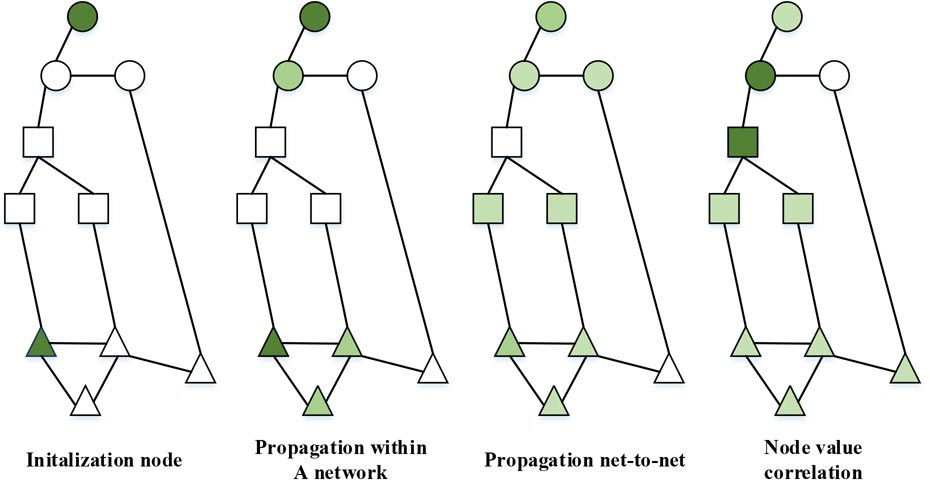
\includegraphics[width = 0.95\textwidth]{workflow}
\caption[fig41]{DrugNet的工作流程}
\label{fig41}
\end{figure}

图中的三角代表通路子网1 ,正方形代表通路子网2,圆形代表通路子网3,节点颜色深浅代表着节点分配的数值 $\psi (v)$,值从0(白)到1(深绿)。查询集合(通路子网1)和目标集合(通路子网3)在初始状况下分数值初值为1查询节点的值从查询节点出发在子网中传播,同样的过程也在目标集所在的子网中传播。从查询网络到目标的网络的路径都会被计算出来(图中只有两条),分数值从查询网络沿着这些路径以式\ref{eq321}和式\ref{eq322}向目标网络传播。该算法的伪代码描述如下:
\\
\\
\\
\\
\\
\\



\begin{algorithm}
 \AlgoBiCaption{DrugNet工作流程}{Workflow of DrugNet algorithm}
\KwIn{G: global graph, Q: query set, $D_{q}$: query network, $D_{t}$: target network)}
\KwOut{Sort list of $D_{t}$ in descending order $L$ }%

Propagate values within $D_{q}$

P:Compute the list of paths from $D_{q}$to $D_{t}$ in G

\For{\emph{each} path pi= {pi1, . . . , pij, . . . , pil} \emph{in} P }
{
	\For {each network $p_{ij}$ in the path $p_{i}$ from $p_{i1}$ to $p_{i(l−1)}$}
	{
		Propagate values from $p_{ij}$ to $p_{i(j+1)}$
		
		Propagate values within $p_{i(j+1)}$
    }

    Store the values of $D_{i(l−1)}$ after propagation through path $p_{i}$ as $\mathnormal{\widehat{x_{i( l-1)} \ }}$
 }

\For{ each entity e $\in V_{t}$ in the target network $D_{t}$}
{
	Set target set $T = {e}$

	Propagate values within $D_{t}$

	Compute correlation coefficient $s_{e}$ using the stored $ \mathnormal{\widehat{x_{i( l-1)} \ }}$ for each path $p_{i}$
}

Sort all entities e $\in V_{t}$ by their sevalues in descending order as L

\end{algorithm}





\section{基于随机游走的通路网络扩展算法}
基于随机游走方法在通路网络扩展和通路中潜在的关联关系的预测应用方面取得了很好的效果。本节将介绍一种改进的随机游走算法kwalk\cite{},该算法在\cite{}中被用于生物通路网络的扩展。

我们在1.2.1中介绍了随机游走的基本概念,在本节中我们将介绍一种有限随机游走,其概念可形式化如下:

令G(V,E)是一个n个节点,m条边组成的图,其中$V=\{v_{i} |i=1...n\}$是顶点的结合,$\ E=\{e_{i} |i=1...m\}$是边的集合。令$A \in R^{n\times n}$是图G的邻接矩阵, $A_{ij}$是邻接矩阵。令$D \in R^{n\times n}$是图G的度矩阵,对角线上的元素是节点的度。定义状态转移矩阵为P。

对于随机游走过程而言
\begin{equation}
	P = AD^{-1}
\end{equation}

为了提高算法的稳定性和健壮性,在有限K步内的随机游走过程状态矩阵定义为
\begin{equation}
	P=(I+A^{-1})(1+D^{-1})
\end{equation}
它考虑到了图中节点有环的情况,但其代价是将所有节点的度都增加了1。

我们定义$x_{i}^{(t)}$为t时刻,游走者待在节点i的概率,i=0,,,n. $x_{i}^{0}$为游走者在节点i 的概率。在游走过程中使用下式计算t+1时刻的概率
\begin{equation}
	x^{(t+1)}=Px^{(t)}
\end{equation}
正常的随机游走,从节点x出发会向整个图游走,但是这种情况耗费了大量的时间并且增加计算量,为了限制游走的范围,获取图的局部结构信息通常使用
 \begin{equation}
 x^{( t+1)} =\alpha x^{( 0)} +( 1-\alpha ) Px^{( t)} \
 \label{lrw}
 \end{equation}
 其中$\alpha$是控制游走范围的参数,使用式\ref{lrw}的原因通常基于一个假设: 游走在游走过程中通常会有较大的概率回到种子节点。

 有限随机游走算法在MCL算法的启发下引入了在每一步转换的膨胀和归一化操作。膨胀操作通常是使用一个超线性函数实现如幂函数:
 \begin{equation}
f( x) =\left[ x^{r}_{1} ,x^{r}_{2} ,x^{r}_{3} ,...x^{r}_{n}\right]^{T}
\label{inflation}
\end{equation}

因为达到每个点的概率必须在区间[0, 1], 在经过膨胀操作之后概率数值会超出这个区间,因此需要对膨胀后的结果做标准化,标准化方法的向量形式可以表述如下
 \begin{equation}
g( x) =\tfrac{x}{x^{T} \ \cdotp \ 1}
 \end{equation}

其中 $1 = [1,1....1]^{T}$。膨胀操作和标准化增加了向量中较大的值,抑制了较小的值。由于我们通过非线性膨胀操作和抑制操作将游走限制在种子节点的领域内,因此我们将上述过程称为有限随机游走(LRW)过程, 算法的伪代码描述如下:
\\
\\
\\

\begin{algorithm}
 \AlgoBiCaption{有限随机游走算法LRW}{Workflow of limited random walk algorithm}
\KwIn{$A$: adjacency matrix of global net $G'(V', E')$, $Q$: seed vertex set,$r$: parameter in equation \ref{inflation}, $T_{max}$: maximum number of iterations, $\epsilon$: a small value for the termination condition}

\KwOut{$x^{(t, i)}$: node vector after limited random walk }%

\For{i $\in$ Q}
{
	initialize $x^{(0, i)}$ such as $x^{\ \ ( 0,i)}_{k}$
    
    \For{$t$=1 to $T_{max}$}
	{
		$x^{(t,i)}=Px^{(t-1,i)}$

		if $x^{(t,i)}_{k} < \epsilon$, let$ x^{(t,i)}_{k}=0 $	

		 $x^{(t,i)}_{k}=f(x^{(t,i)}_{k}=(x^{(t,i)}_{k})^{r}$

		 $x^{(t,i)}_{k}=g(x^{(t,i)}_{k})$

		if  $x^{(t,i)}_{k} -  x^{(t,i-1)}_{k} < \epsilon$ break

 	}
}


\textbf{return} $x^{(t, *)}$
\end{algorithm}


\section{基于搜索策略的生物通路网络扩展算法}
基于搜索策略的生物网络扩展算法主要的观点是将生物通路网络作为种子网网络映射到全局网络中,从种子网络的节点出发进行基于某种策略的搜索,将全局网络上搜索的节点作为扩展后的节点加入到生物通路网络中。

在搜索过程中,选取那些节点纳入扩展后的生物通路网络中,需要考虑到扩展的条件,如果选择的扩展的条件不当,会造成纳入生物通路网络中的节点过多,而部分纳入的节点是与原来通路网络关联并不强。而扩展生物通路网络需要考虑到网络的拓扑结构特点,因此需要考虑生物通路网络的特征。

结合第二章对于290张生物通路网络分析结果可知,这290张生物通路具有小世界网络的特点,小世界网络里大部分结点可以从任一其他点经少数几步就可到达,聚集系数能反映节点邻居的邻居和该节点的相关程度,因此可以选择聚集系数作为扩展的条件,记节点x的聚集系数为CC(x)。

同时生物通路网络还需要考虑在生物层面的作用强度,因此生物层面节点作用强度也需要作为扩展的条件,在第二章网络网络创建部分我们使用的权重就是通路网络中节点在生物层面的强度信息。

算法的过程可以形式化如下:令G(V,E)是一个n个节点,m条边组成的图,其中$V=\{v_{i} |i=1...n\}$是顶点的结合,$\ E=\{e_{i} |i=1...m\}$是边的集合, $w_{ij}$是节点i 与节点j 之间的权重。$L= \{l_{ij} | i=1...n, j=1...n \}$,其中$l_{ij}$是节点i和节点j之前的路径, $l_{ij}$实际上是节点i和节点j的边的集合,即$l_{ij}=\{e_{ip} , e_{pq}, e_{ql}...e_{kj}, p,q,l,k\in Z^{+} p,q,l,k < n \}$。$N_{l_{ij}}=\{v_{i}, v_{p}, v_{q}, v_{l}...,v_{k},...v_{j}\}$, 是路径$l_{ij}$上所有的节点。记$G^{'}(V', E')$为全局网络,如第二章所述我们使用HumanNet作为全局网络。

选$\forall x\in V$开始深度优先搜索,当搜索到节点y时,基于聚集系数衡量x与y之间的关联程度可计算为 
 \begin{equation}
\ S_{xy} =\prod _{v\in N_{l_{xy}}} CC( v)
 \end{equation}

选$\forall x\in V$开始深度优先搜索,当搜索到节点y时,基于生物层面衡量x与y之间的关联程度可计算为 
 \begin{equation}
\ S'_{xy} =\prod _{e\in l_{xy}} w( e)
 \end{equation}
其中w(e)是边e在全局网络上的权值。

选$\forall x\in V$开始深度优先搜索,当搜索到节点y时,需要判断搜索到的节点y是否被纳入扩展后的网络,需要判定函数进行判定,当 $S_{xy}$或$S_{xy}$大于给定阈值$\theta$时,判定函数输出为1,节点y被纳入生物通路网络;当 $S_{xy}$或$S_{xy}$小于给定阈值$\theta$时,判定函数输出为0,节点y不被纳入生物通路网络,对其后续节点的搜索这时也将停止,数学表述如下式:
\begin{equation}
f( x) =\begin{cases}
0 & S_{xy} < \ \theta \ and\ S^{'}_{xy} < \ \theta \ \\
1 & otherwise
\end{cases}
\end{equation}

如图\ref{algorithm}所示,图中节点的数字代表其该节点的聚集系数,图中红色节点时当前访问的节点,图中蓝色的节点是生物通路网络中的节点(种子网络节点)。我们选择A节点做作为搜索的源点对全局网络$G^{'}$进行深度优先搜索,选取的阈值$\theta=0.8$,。当访问到的节点$v\in E$时,也就是v是种子网络的节点时,搜索过程继续;当访问的节点不是种子网络的节点时如D、E、F、G、H时,分别计算法其聚集系数关联$S_{xy}$、生物层面的关联$S'_{xy}$,使用判别函数进行计算,若判别函数输出为1时将节点纳入生物通路网络如节点G。将V中所有的节点作为搜索源点,重复如上的操作,最终即可获得扩展后生物通路网络,算法的伪代码如下:


\begin{algorithm}
 \AlgoBiCaption{基于深度优先搜索的通路网络扩展算法}{Depth-first based pathway network expansion algorithm}
\KwIn{$G^{'}(V', E')$: global network, $V$: vertex set of pathway network, $\theta$:cutoff of expansion nodes}
\KwOut{$M$: expansion node set }%

\For{ \textbf{each} x in V } 
{
	Let $S$ be a stack
	
	S.push(x)
	
	\While{S is not empty}
	{
		v = S.pop()

        \If{v is not labeled as discovered}
        {
        	Label v as discovered

        	\For{ all edges from v to w in G.adjacentEdges(v) } 
        	{
        		\If {w is not labeled as discovered} 
        		{
        			S.push(w)
        		}
        	  	
        	}

        	Calculate  $S_{xv}$ and $S'_{xv}$
        	
        	\If{$S_{xv}$ < $\theta$ and $S'_{xv}$ < $\theta$} 
        	{
        		M.push(v)
        	}
        }
	}

	S.clean()
}
\end{algorithm}
\newpage

\begin{figure}[h]
\centering
\includegraphics[width = 0.82\textwidth]{algorithm}
\caption[algorithm]{基于深度优先搜索的生物通路网络扩展算法的工作流程}
\label{algorithm}
\end{figure}


 \section{实验结果}
 我们使用HumanNet作为全局网络,按照上一章的提出的网络构建方法,选取290个人类相关的通路作为研究对象,对这290个生物通路网络进行了扩展,为了验证实际的扩展效果并方便讨论分析,我们选取文献\cite{},列出的15个人类乳腺癌相关的通路作为本章讨论重点的研究对象。
 \subsection{扩展结果分析}
 我们使用以上3.2-3.5章中介绍的算法进生物通路网络的扩展,从扩展后节点的数量以及扩展网络的准确度方面进行讨论。我们在图\ref{allexpansion}列出
 \begin{figure}[h]
\centering
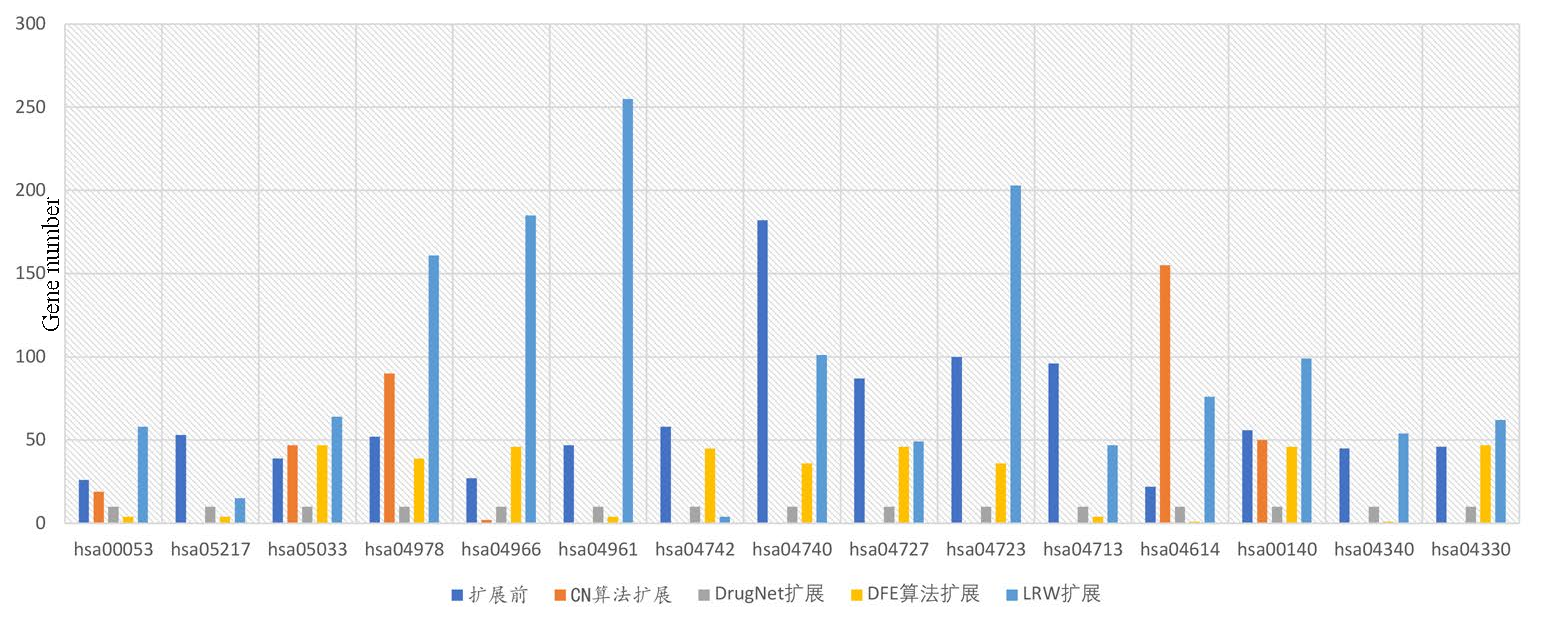
\includegraphics[width = 0.95\textwidth]{allexpansion}
\caption[allexpansion]{15个癌症相关生物通路网络的扩展结果}
\label{allexpansion}
\end{figure}

我们扩展了hsa00053在内的15个KEGG\cite{}生物通路,从数量角度可以对扩展结果进行简单分析。
图中“扩展前”图例代表通路在扩展前的规模,而算法扩展的柱状图高度代表该在该生物通路网络上运行该算法后扩展的节点数量。由图\ref{allexpansion}可知,CN算法对于生物通路扩展的效果较差。在15个通路网络中, CN算法不能对其中9个通路网络
进行有效的扩展,在扩展过程中,没有任何节点被纳入通路网络中,与我们上一章分析节点一致,该算法的效果取决于其所扩展的网络。

DrugNet算法扩展效果比较稳定,对于每张网络均有10个新的节点纳入到生物通路网络中,但是其纳入的节点数量和网络的规模没有明显的关联,因此对于有些节点较多的网络而言,该算法可能遗漏部分重要节点。同时,DrugNet在进行扩展时需要选择通路网络部分节点作为网络信息传播的源点,因此这些节点的选取可能对扩展的效果有影响。


LRW算法扩展后纳入的节点较多,部分通路网络扩展后新纳入的节点数目远远超过了网络自身的规模如hsa04961, hsa04723, hsa04966等,LRW扩展这些通路网络后纳入的节点数目是通路网络节点数目的2-4倍, 纳入更多的节点意味着更多的计算量和时间开销,因此可能对算法的时间效率有影响。同时,纳入节点导致验证这些节点和通路网络之间的关联成为了挑战。

DFE算法纳入节点数目和LRW相比较少,但是其扩展的节点数目和网络规模有关联,这一点比DrugNet考虑的更全面,同时选择合适的参数将网络扩展后规模控制在合理的范围内,有利于验证这些扩展后节点与通路之间的关联。

\subsection{扩展结果验证}
为了验证算法扩展的节点是否与乳腺癌相关,我们选取BRCA数据集来验证通路扩展的结果。BRCA数据集是从癌症基因组网站TCGA(英文名全称:The Cancer Genome Atlas,网址为http://cancergenome.nih.gov/)下载的数据。该数据由于数据质量较好,被广泛的应用于癌症通路的识别,药物靶点发现,药物重定位的研究。

记扩展后基因的集合为$g_{e}$, BRCA中的基因集为$B$, 使用下式来衡量扩展的效果
 \begin{equation}
r\ =\ \frac{||g_{e} |\ \cap \ |B|}{|g_{e} |}
 \end{equation}
r的值实际上代表扩展基因里乳腺癌基因所占比率,比率越高说明扩展的效果越好。我们统计了以上4种算法在BRCA数据集上的验证结果
\begin{figure}[h]
\centering
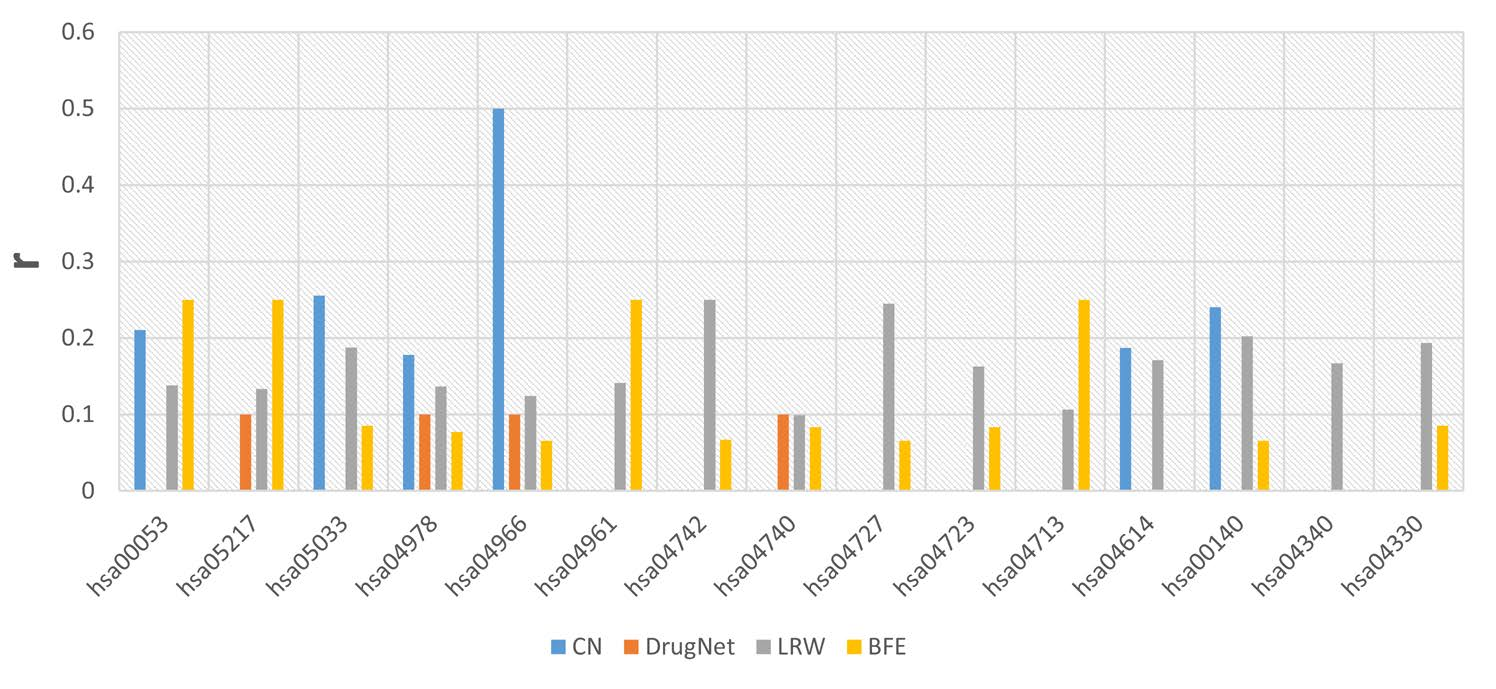
\includegraphics[width = 1.0\textwidth]{rate}
\caption[rate]{扩展后的基因里乳腺癌基因所占比率}
\label{rate}
\end{figure}

由图中可知DrugNet算法扩展后的节点很少是乳腺癌基因,DrugNet扩展效果不佳。CN算法在某些通路网络上取得了较好的效果,但是在大部分的生物通路网络上效果不佳,说明CN算法很依赖网络结构。LRW和BFE的扩展效果比较稳定,在15张通路网络上均取得比较好的效果,LRW扩展的节点中乳腺癌基因的比例更高。


 \subsection{性能评价}
 为了验证算法的性能,我们对以上的算法进行了性能测试,我们选用留一交叉验证法(Leave-One-Out Cross Validation)记作LOO-CV。LOO-CV测试过程如下:如果设原始数据有N个样本,那么LOO-CV就是每个样本单独作为验证集,其余的N-1个样本作为训练集,所以LOO-CV会得到N个模型,用这N个模型最终的验证集的分类准确率的平均数作为性能指标。

 采用上述的验证方法保证了所有的样本都参与了模型训练,因此最接近数据最原始的分布,验证的结果比较可靠。排除了随机因素对于实验结果的影响,保证了结果是可以复制的。对于待验证的通路网络G(V, E),我们每次选择一条边移除,若算法能正确地将其扩展到通路网络里,我们认为本次扩展是成功的。重复进行以上的操作$|E|$次,其中有m次能正确的扩展到通路网络中,我们定义预测的准确度

\begin{equation}
precision\ =\ \frac{m}{|E|}
\end{equation}
我们对以上四个算法进行该测试,得到如下的测试结果:
\begin{figure}[h]
\centering
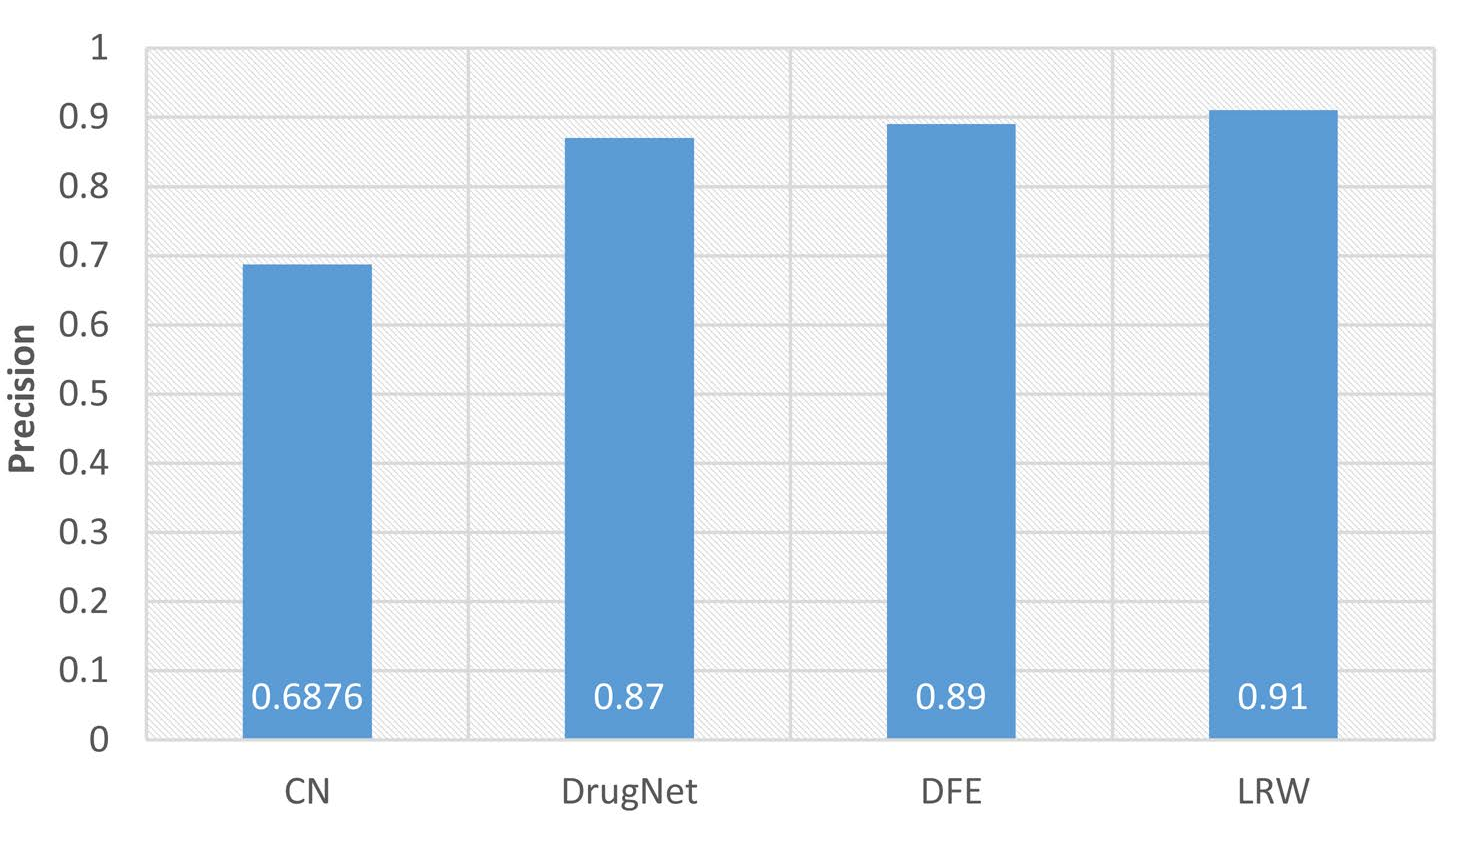
\includegraphics[width = 0.8\textwidth]{precision}
\caption[precision]{算法的精度验证结果}
\label{precision}
\end{figure}

由测试结果可知,CN算法的网络扩展的精度较差只有0.69,这与上一节的实验结果分析一致。由于生物通路网络具有小世界特性和无尺度的特点,而CN算法在生物通路网络上能获取的信息有限,因此其CN算法不适合通路网络的扩展,DrugNet和DFE算法网络扩展的精度都较高,DFE略高于DrugNet。LRW 算法的扩展效果最佳,其网络扩展精度可达0.91。

\subsection{运行时间分析}
算法在在实际的应用中,需要考虑到算法效果和时间效率的平衡。因此对于算法运行时间的分析对于算法性能的比较和算法性能的改进十分重要。我们在15个人类乳腺癌相关的通路网络上运行了以上四个算法,得到了网络规模和运行时间之间的折线图\ref{runtime}, 由于LRW运行时间很长与CN,BFE, DrugNet的不在同一个数量级,为了直观进行对比,图\ref{runtime}采用了双坐标轴。右边的纵坐标轴表示LRW的运行时间,左边的纵轴表示其他3个算法的运行时间。
\begin{figure}[h]
\centering
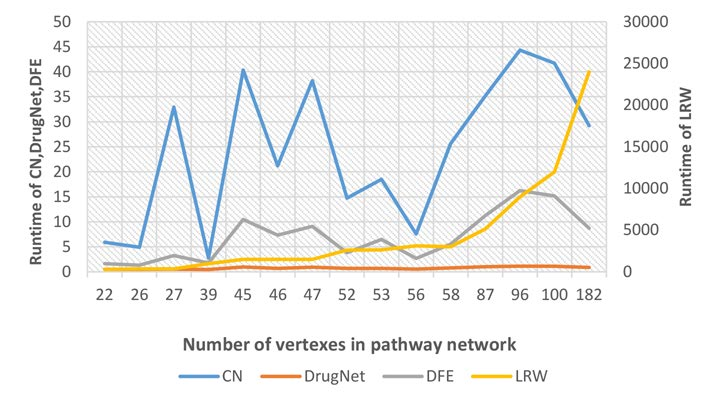
\includegraphics[width = 1.0\textwidth]{runtime}
\caption[runtime]{算法的时间性能分析}
\label{runtime}
\end{figure}

由图可知LRW算法是最耗时的,随着网络规模的增加其运行时间呈现出指数型的增长趋势,当网络的规模增加到100时,其运行时间达到1300多秒。下面我们对从算法的时间复杂角度进行简要分析。对于每个顶点,每次迭代都涉及到转移矩阵$P$和概率向量$x$的乘积。我们注意到在游走过程中不仅仅访问节点自身,而且访问节点附近一定数量的节点,因此极大的增加了计算量。同时膨胀过程也涉及到矩阵乘积的计算,随着节点规模的增加,矩阵的乘积计算量会指数型增长因此时间开销会极大增加。其时间复杂度最坏情况下为$O(n^{3})$(详细的时间复杂度分析可以参见\cite{})。

CN算法的运行时间较长,原因是在于CN算法需要计算所有节点两两之间的公共邻居矩阵,因此计算次数为$|V|*|V|$, 对于无向图而言其计算次数为$\frac{|V|*|V|}{2}$, 由于生物通路网络具有小世界的特点,当通路中的节点n增大时候,|V|趋近与全局网络的边集的基数$|V^{'}|$,因此随着网络的节点增加计算的时间急剧增加。因此计算的复杂度为$O(n^{2})$。

DFE基于深度优先遍历算法,深度优先遍历算法时间复杂度为$O(|V| + |E|)$, 由于把对V中所有当做深度优先搜索的源点,因此总的时间复杂度为$O((|V| + |E|)*|V|)=O(n^{2})$

DrugNet算法复杂度为$O(n^{3})$, 但由于复杂度取决于种子网络,因此在图\ref{runtime}中该算法的计算速度很快。

% \subsection{案例研究与文献验证}
\subsection{本章小结}
在本章中,我们在15个人类乳腺癌相关的生物通路网络上比较了4种生物通路网络扩展算法,实验结果表明在这些通路网络上有限随机游走算法(LRW)和基于深度优先遍历(BFE)的扩展算法扩展效果较好,扩展后的一部分节点可以在公开的乳腺癌数据上得到验证。在时间性能方面,基于深度优先遍历(BFE)的扩展算法和DrugNet算法有较好的时间性能,但是DrugNet扩展结果只有很少数在乳腺癌数据集中。综合扩展的效果和时间性能,我们在本章提出的基于深度优先搜索的通路网络扩展算法具有较好的效果。




\chapter{生物通路网络可视化系统}
\section{引言}
随着生物信息学高速发展,大量的实验数据迅速积累,由于数据规模日益增大,使用网络的方法来研究这些数据已经成为了很多研究使用的方法。对蛋白质网络、基因调控网络、代谢网络、生物通路网络的研究日益深入,对于这些网络可视化的需求日益增长,同时这些大量的网络数据也促进了可视化技术的研究。设计良好生物通路网络可视化系统,有助于帮助研究者直观深入地了解复杂的内部结构,有助于揭示这些数据背后蕴藏的生物意义。

在传统的情况下,生物通路网络一般是由生物学专家来绘制,数据库中展示的生物通路图也是静态的不可以编辑的。这种方式很耗时耗力,当发现一个通路中有新的信息时候,更新生物通路十分耗时。随着互联网技术发展和大数据时代的到来,数据的可视化技术日益成熟。互联网时代研究者对于数据的快速获取和分析需求日益增长,而目前主流的可视化系统存在的问题在于大部分是桌面端的软件,这些软件在配置使用上为研究者增加了时间成本。部分商业化的可视化系统存在着授权费高昂、数据导出限制等问题,因此急需开发一款能让研究者快速访问并使用,且能节省使用者时间和资金成本的可视化系统。

本章中我们将介绍一款基于Web技术的生物通路网络可视化系统。我们将在本章详细介绍其软件架构、系统功能模块划分、系统实现技术。

\section{软件架构}
通路网络可视化系统的整体架构如图\ref{fig31}, 整体架构包含三个层级操作系统层,支撑软件层, 应用软件层。操作系统层为整个系统提供最基础的资源,为整个系统实现了资源调度分配和管理,由于采用基于Web技术B/S架构因此和操作系统种类无关,操作系统的种类并不影响整个系统的使用。

支撑软件层为整个系统提供了运行的环境,基础的API,系统基本的页面框架,由于使用Python 作为后台支撑软件编程语言,因此可以既可以实现页面请求的处理,又可以进行大规模数据的处理。由于系统中使用到的数据是关系型的数据,因此数据库层面使用了被网页开发广泛使用的MySQL数据库。

应用软件层实现了整个软件的系统功能。其应用软件层包含三个子模块分别是Handlers、Methods、Mappers。Handler模块的主要功能是响应浏览器端的请求。SearchNetHandler的作用是当用户输入某些实体关键词时,后台响应用户请求,在数据库中的全局网络上检索和输入实体相关的生物通路网络结构信息。VersionHandler的作用是当用户检索到网络数据后进行数据封装、序列化等操作,同时将序列化后的数据在前端和展示控件进行映射展示。DrugHandler主要响应用户药物实体检索请求。GenePathwayHanlder主要响应用户的基因和通路检索请求。Mapper模块主要作用是将数据库中的查询信息到Hanlder模块所需的数据结构间的映射。由于使用了ORM技术,用户查询到的结果都是以对象的形式返回如基因信息对象Geneinfo等,而前端需要结构化的信息,因此mapper模块承担了这个任务。Method模块封装了系统中的帮助类如按照Cytoscape格式进行数据打包,部分数据的清洗转换,数据操作类的封装,Versionutils和Simulation子模块承担了这部分的功能。
\begin{figure}[h]
\centering
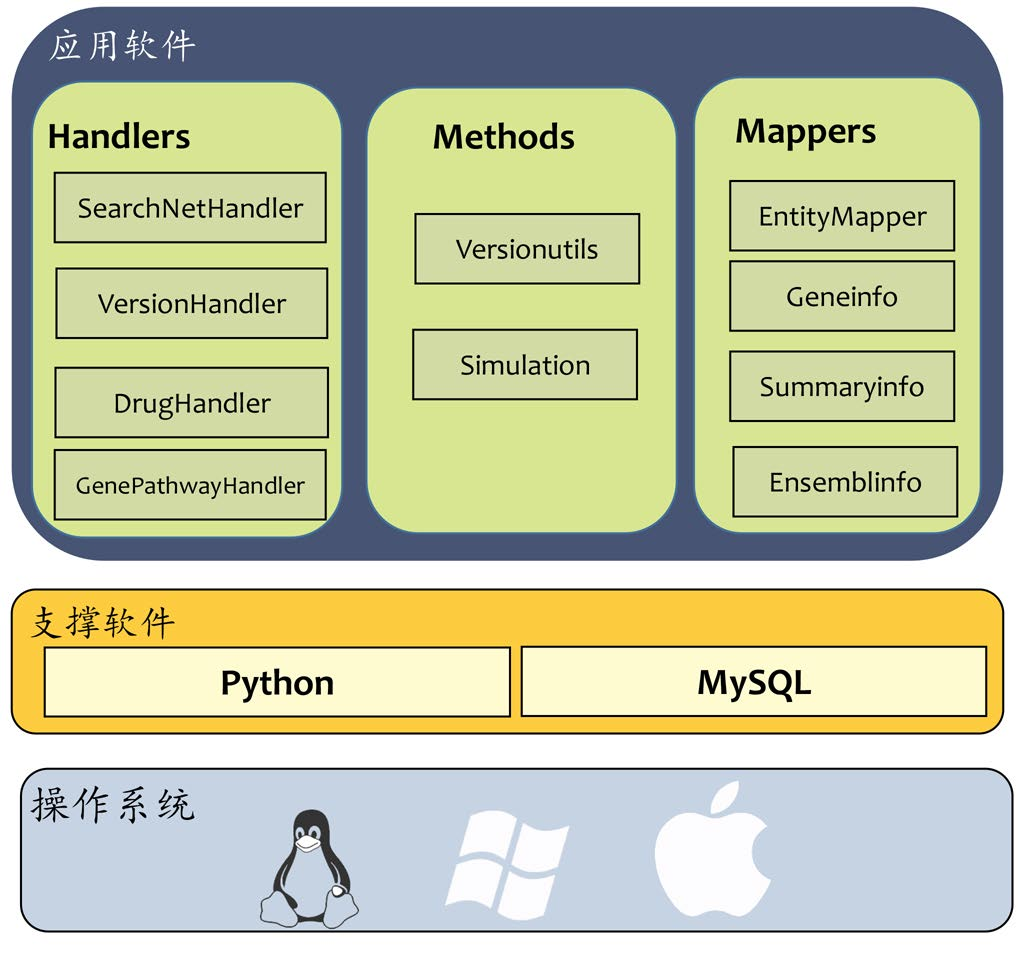
\includegraphics[width = 0.8\textwidth]{framework}
\caption[fig31]{可视化系统的架构}
\label{fig31}
\end{figure}

\section{系统功能模块划分}
本系统设计目的旨在使用网络可视化技术将用户检索的信息进行直观的展示,用户和与系统之间有良好的交互,用户可以在系统中直观地快速地获取自己想要的信息。同时系统还支持网络信息图片格式导出,供用户在下载和使用,该部分对标IPA的基因网络可视化模块,经过前期调研IPA系统使用了商业公司开发的可视化系统,这些系统和软件库授权往往十分昂贵,而我们的系统是开源的,用户使用过程中无任何的经济负担,这是该系统的一大优势。同时,我们的系统关联了丰富的数据库,用户可以便捷的检索到自己想要的信息,免去了自己去收集整理信息的过程,节省了用户的使用时间。

本系统按照功能可以划分为三个主要的模块如图\ref{fig32}所示,分别为:概要信息展示模块、详细信息展示模块,网络可视化模块。在我们的系统中这三个模块分别对应三个面板如图\ref{UI},这三个面板为用户提供信息的展示和交互。

\begin{figure}[h]
\centering
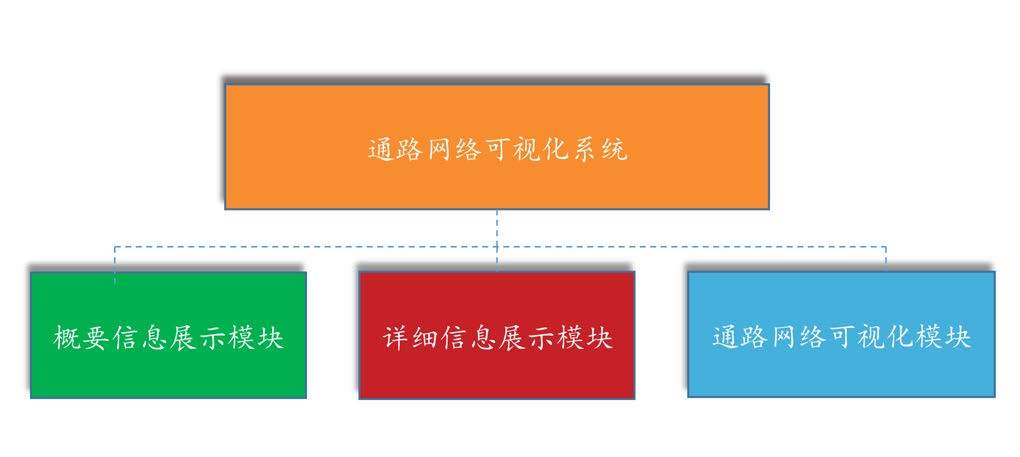
\includegraphics[width = 0.8\textwidth]{module}
\caption[fig32]{系统功能模块划分}
\label{fig32}
\end{figure}

概要信息展示模块旨在为用户展示最直观、最重要的信息。当用户选中网络中的某个元素时(节点或者边)时,该模块会展示与选中元素关联的最为重要的信息。生物通路网络的基本统计信息也由该模块给出,为用户提供对生物通路网络最直观的认识。用户想修改选中元素的属性时,该模块也为用户提供样式的修改功能。

详细信息展示模块旨在为用户展示选中元素关联的详细信息。本系统中生物通路网络默认的节点是基因,当用户点击某个节点时,与该节点相关的基因信息、疾病信息、药物信息、通路信息、基因表达信息、网络分析结果信息等都会在该模块以表格和统计图等形式给出。该模块建立起基因、疾病、药物、通路等数据之间的关联,对于数据整合具有重要的作用。

网络可视化模的主要的功能是对检索到的信息进行网络化展示,该模块也是整个系统的核心模块。其子模块被整合到工具栏中供用户的使用。 该模块承担着系统与用户交互的任务,用户可以对网络进行自定义的编辑,对网络中节点和边进行样式的手动修改,并支持以图片格式导出。



\begin{figure}[h]
\centering
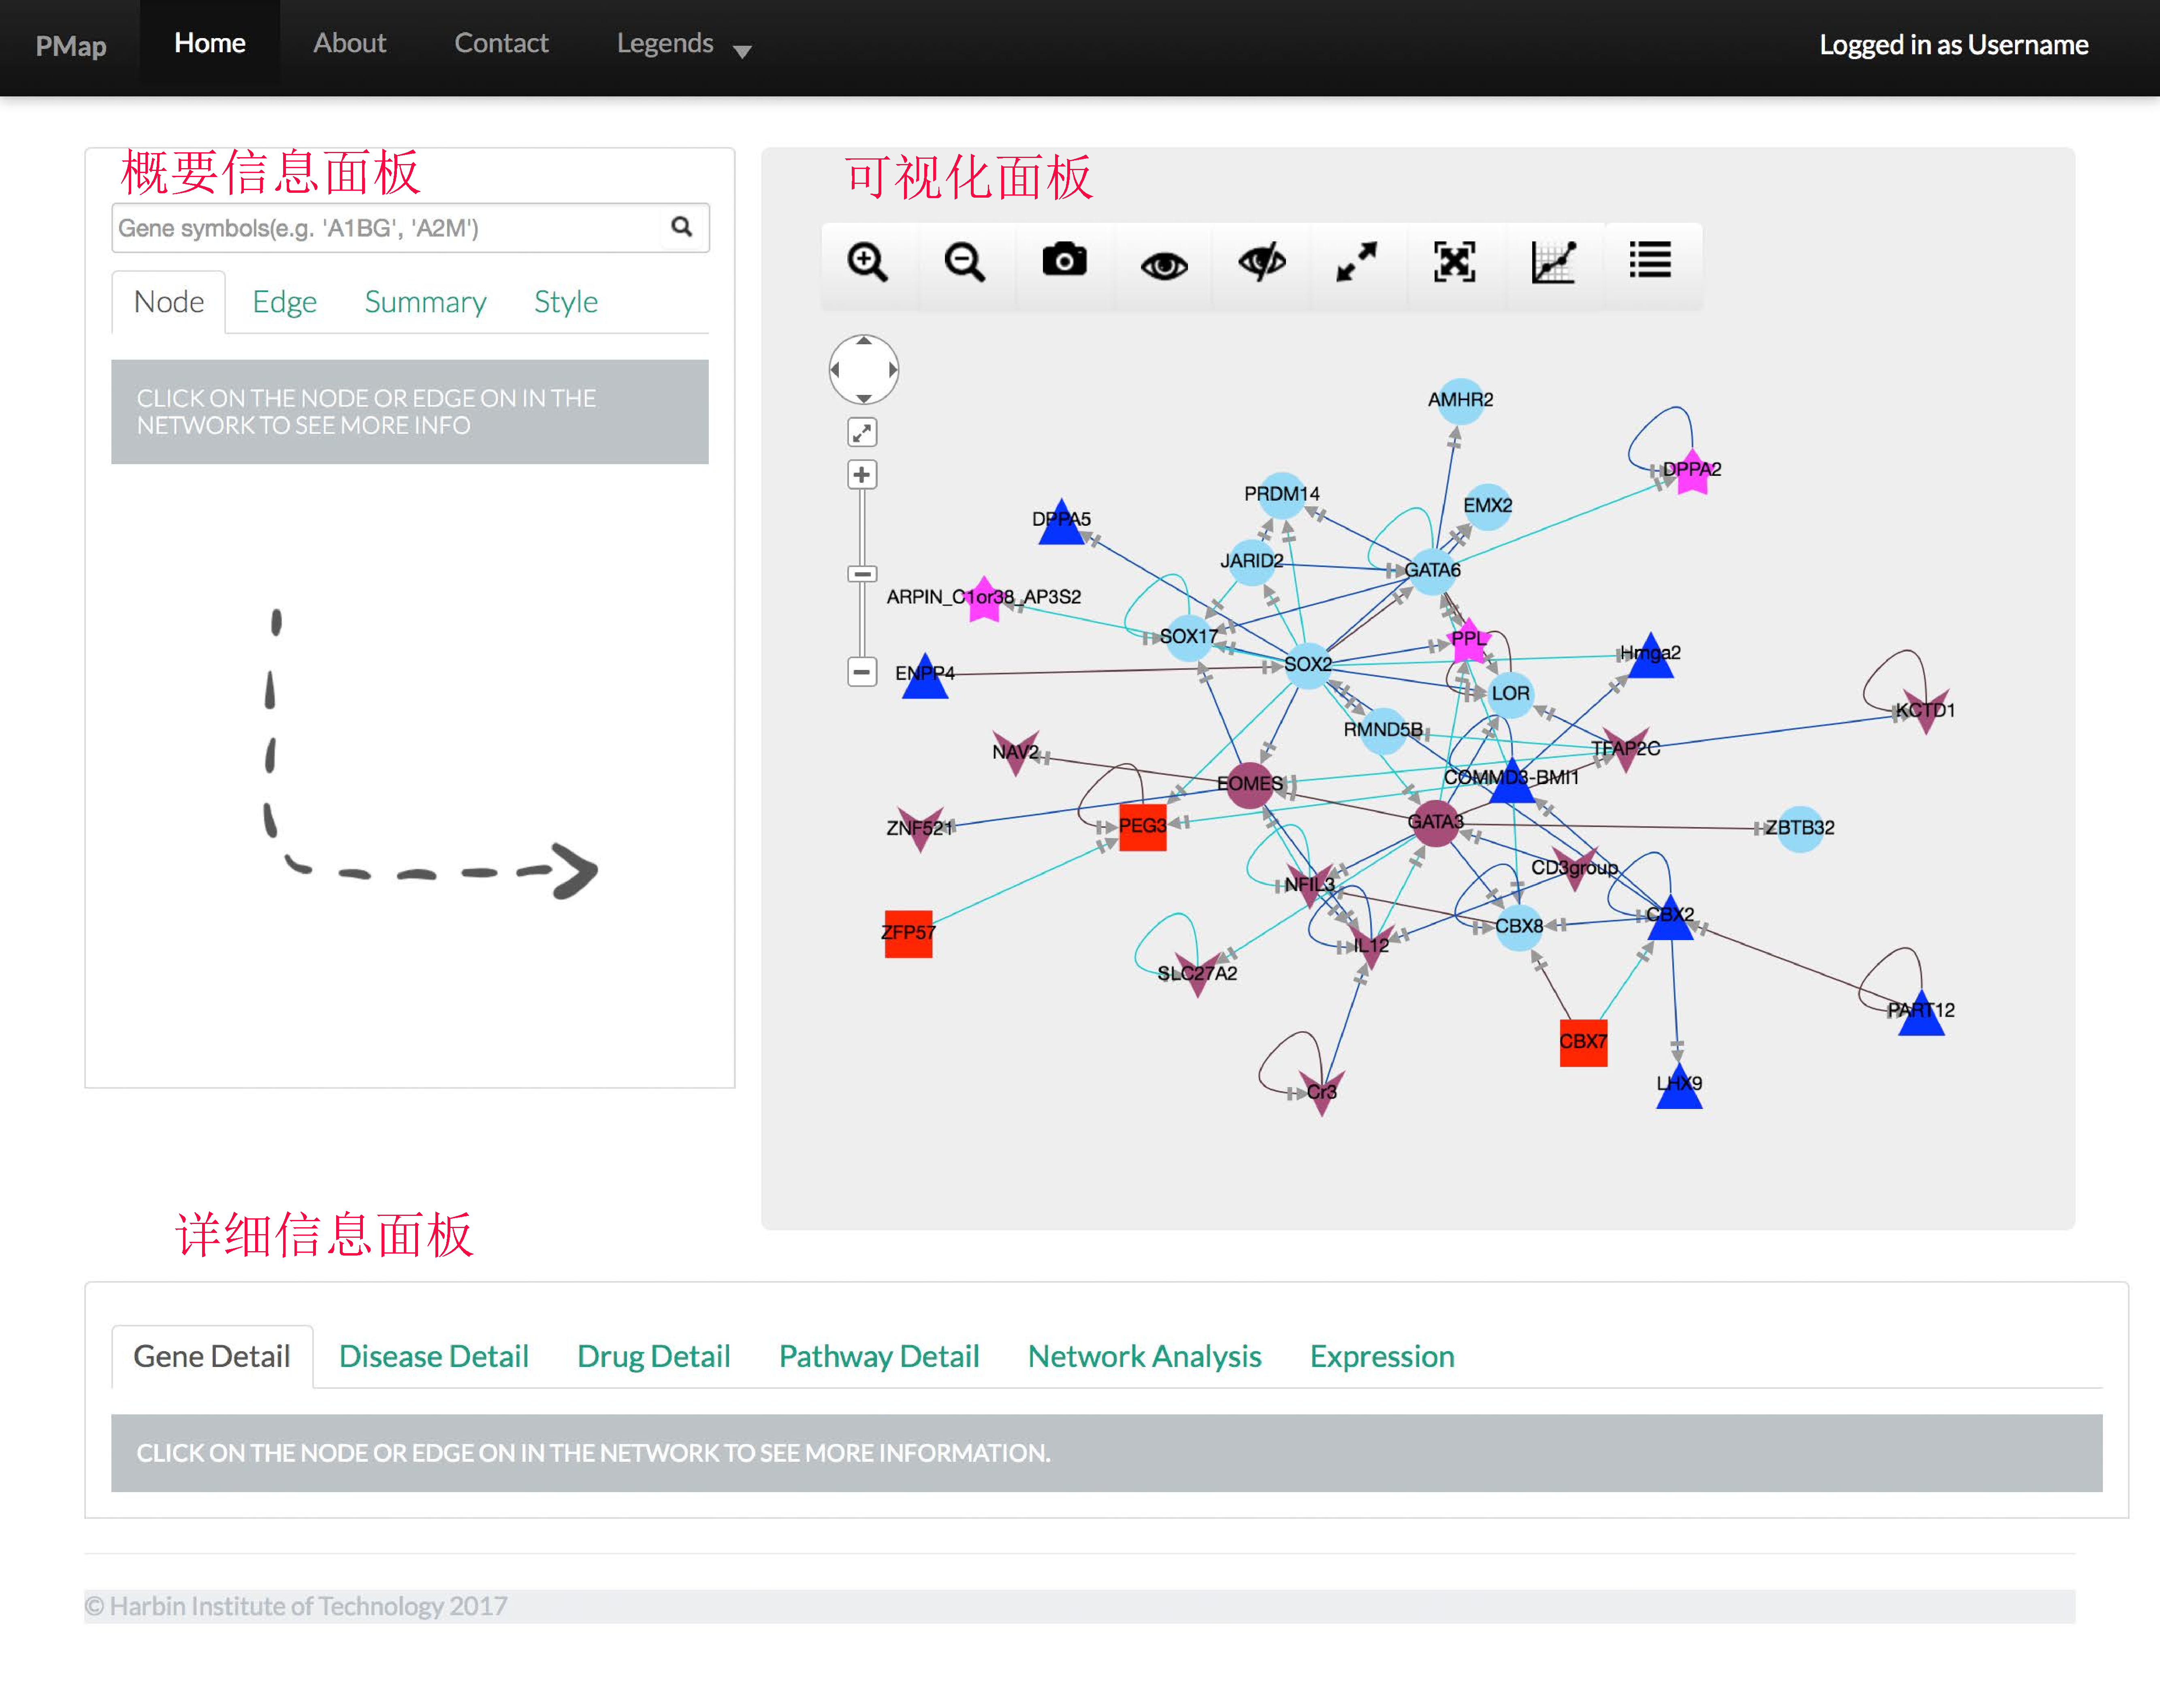
\includegraphics[width = 1.0\textwidth]{UI}
\caption[UI]{系统主界面}
\label{UI}
\end{figure}

\subsection{网络可视化模块}
网络可视化模块是本系统的核心模块,该模块实现了对网络的可视化展示,网络相关的操作、网络布局调整、 网络最大化、网络的分析等。具体而言该模块可以分成:网络放大、网络缩小、网络导出、网络布局调整、节点显示、节点隐藏、网络分析、网络最大化等八个子模块。该部分功能是对Cytoscape在浏览器端编程接口进行封装而实现。 

网络放大、网络缩小、网络最大化是对网络操作的一部分。其实现方式通过两种途径,一种是通过工具栏中相关的按钮,另一种是通过网络控制盘。当用户点击某个网络中元素(边和节点)时,如果用户想隐藏该节点可以通过点击工具栏隐藏按钮,用户想恢复这些节点时可以点击工具栏显示按钮,用户选中某个子网络时,也可以对选中的子网中进行隐藏和显示。如果用户对系统当前的网络满意时,系统提供了以图片格式导出网络功能,用户可以点击下载按钮得到该网络对应的图片。

网络分析模块为用户提供了对生物通路网络的在线分析功能。分析的内容包括度分布分析、最短路径分析等,当用户节点网络分析按钮时,系统进行异步响应,将网络数据提供给后台,经过后台功能模块处理后返回前端以统计图的形式进行展示。

由于生物通路网络具有复杂的结构特性,因此对于生物通路网络的展示效果取决于网络的布局。本系统提供9种布局算法:随机布局、水平布局、环状布局、中心性布局、广度优先布局、Cose布局、分散布局、Dagre布局、Arbor布局(如图\ref{layout})。以下我们将对这9种布局进行详细介绍:

随机布局:随机布局是生物通路网络最基本的布局算法,系统获取展示面板的宽度和高度后,随机为网络中的节点分配坐标信息,该布局算法适用于节点较少,边稀疏的网络。

水平布局:水平布局适用于规模较大的网络,当网络中节点和边的规模很大时,节点和边过于杂乱,使用水平布局可以使得网络有序、简洁,网络中度较大的节点在水平布局时能被迅速发现。

环状布局:网络中所有的节点按照网络中节点度的大小排布在一个圆环上,在这种布局下度较大的节点能被迅速发现。和水平布局相似,这种布局也会使得网络有序、简洁。这种布局适用于节点和边稠密的网络。

中心性布局:中心布局适用于边稀疏且具有少量的核心节点的网络,这种布局会将核心性最重要的节点放在展示面板中央,用户能迅速发现网络的核心节点或核心节点组成的子网。

广度优先布局: 广度优先的概念来源于图论中广度优先遍历的概念,使用这个布局算法时实际上为待布局的网络实施广度优先遍历算法,得到了该网络广度优先遍历的顺序信息,根据遍历的顺序信息为网络中的节点分配位置信息。该算法适合于存在流特点的网络,对于生物通路网络而言,生物信息通路网络符合这种特性。

Cose布局: 该布局是Begum\cite{An algorithm for automated layout of process description maps drawn in SBGN} 等人针对生物网络设计的一种布局算法。该布局力图使整个生物网络呈现清晰的结构特点。该算法改进了弹簧布局\cite{Spring layout}模型,其主要观点是选取网络中的某些种子节点,将这些种子节点进行扩展使得种子节点的邻居都处于一个紧密的小子网里,得到这些子网后为子网们分配位置,该方法强调网络的结构信息,对于由致密的小子网构成的网络,该算法具有很好布局效果。

分散布局:该布局适用于边稀疏并且网络中存在部分重要的节点,该布局以这些节点为中心,将其邻居分散排布在其周围的环状区域内,该布局突出了网络中某些节点的重要性。

Dagre布局:该布局和深度优先布局类似,适合于网络存在流状的结构和路径的网络,对于生物信号通路网络该算法具有较好的效果,dagre布局来源于依赖图的绘制,因此对于节点间有依赖关系的结构网路具有很好的效果。

Arbor布局:该布局观点来自物理学中的万有引力和胡克定律,将网络中所有的节点看成带点粒子,粒子间既存在引力也存在斥力,将整个网络看成一个系统后,当系统内所有粒子间的引力和斥力相互抵消达到平衡时,整个系统趋于稳定,系统稳定后所有节点的位置信息也就被计算出来了。该算法适合于规模较大网络。

\begin{figure}[h]
  \centering
  \begin{minipage}{1.0\linewidth}
    \setlength{\subfigcapskip}{-1bp}
    \centering
    \begin{minipage}{\textwidth}
      \centering
      \subfigure{\label{juti1}}\addtocounter{subfigure}{-2}
      \subfigure{\subfigure[随机布局]{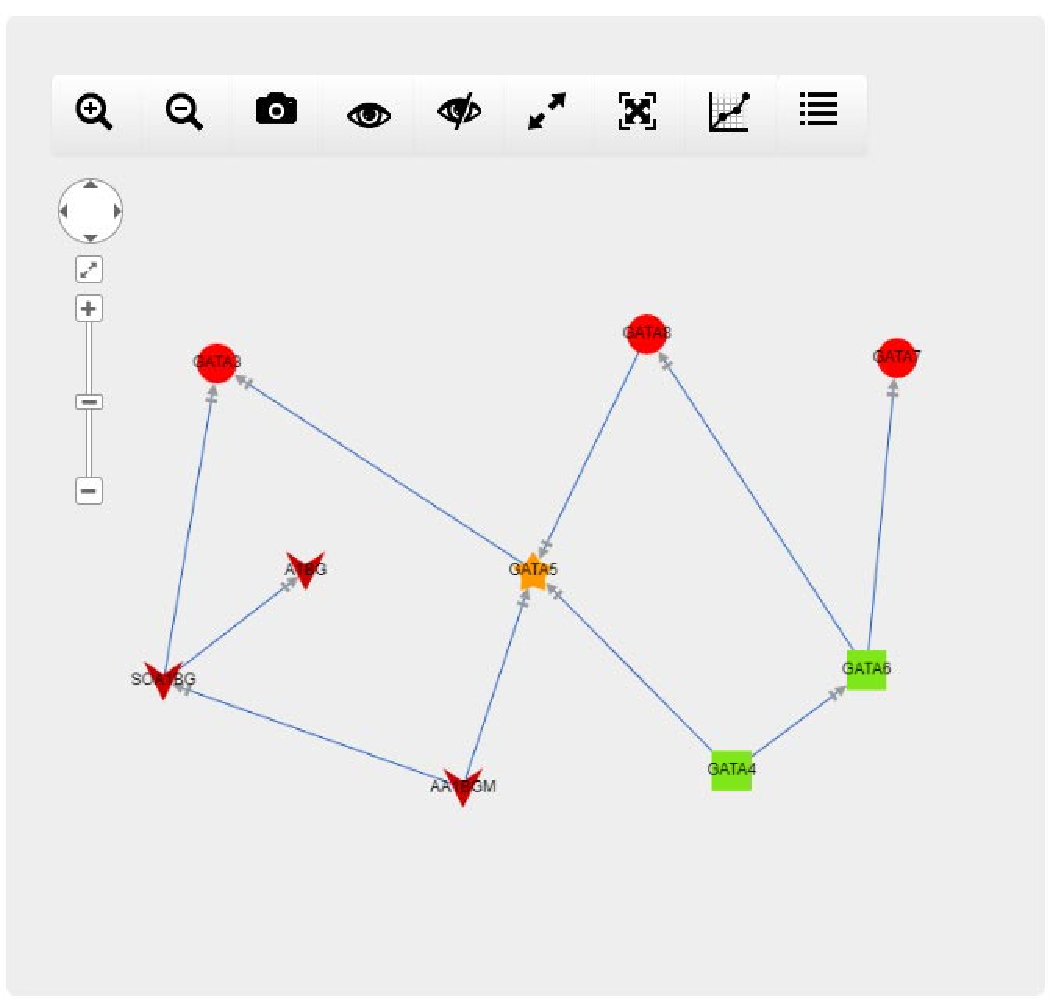
\includegraphics[width=0.3\textwidth]{l1}}}
      \subfigure{\label{juti2}}\addtocounter{subfigure}{-2}
      \subfigure{\subfigure[水平布局]{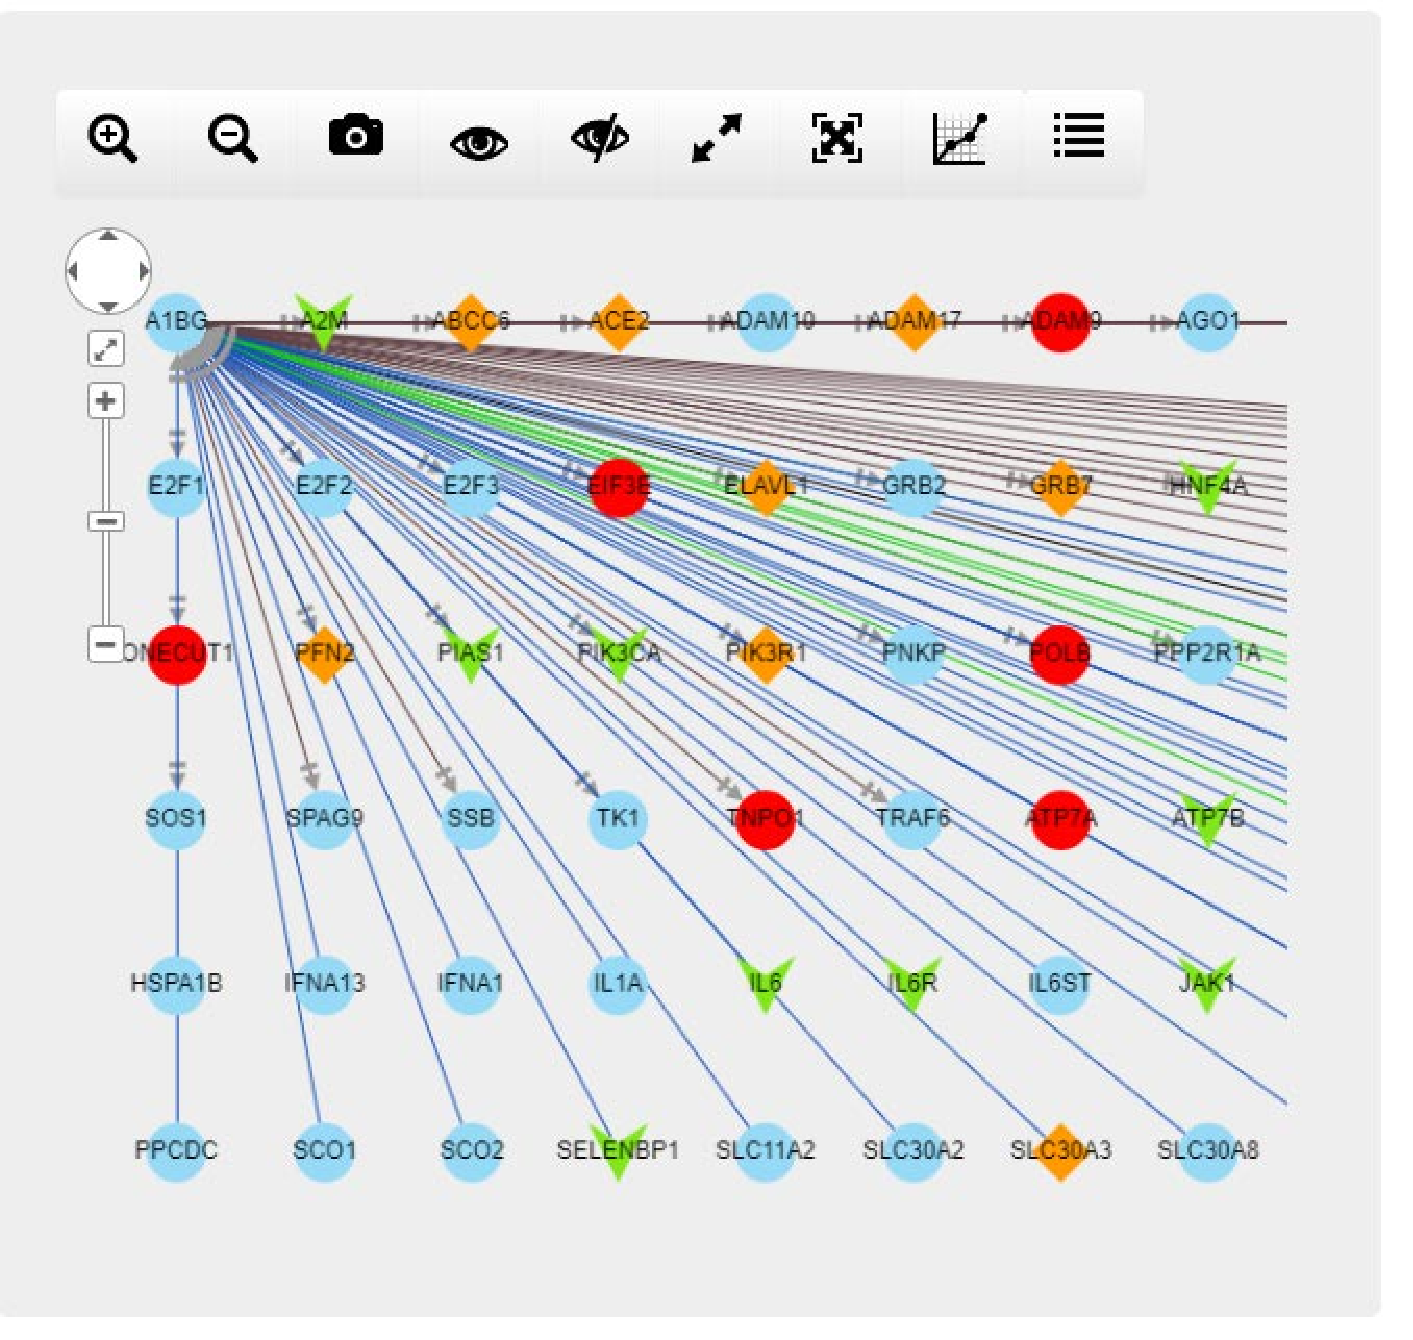
\includegraphics[width=0.3\textwidth]{l2}}}
      \subfigure{\label{juti3}}\addtocounter{subfigure}{-2}
      \subfigure{\subfigure[环状布局]{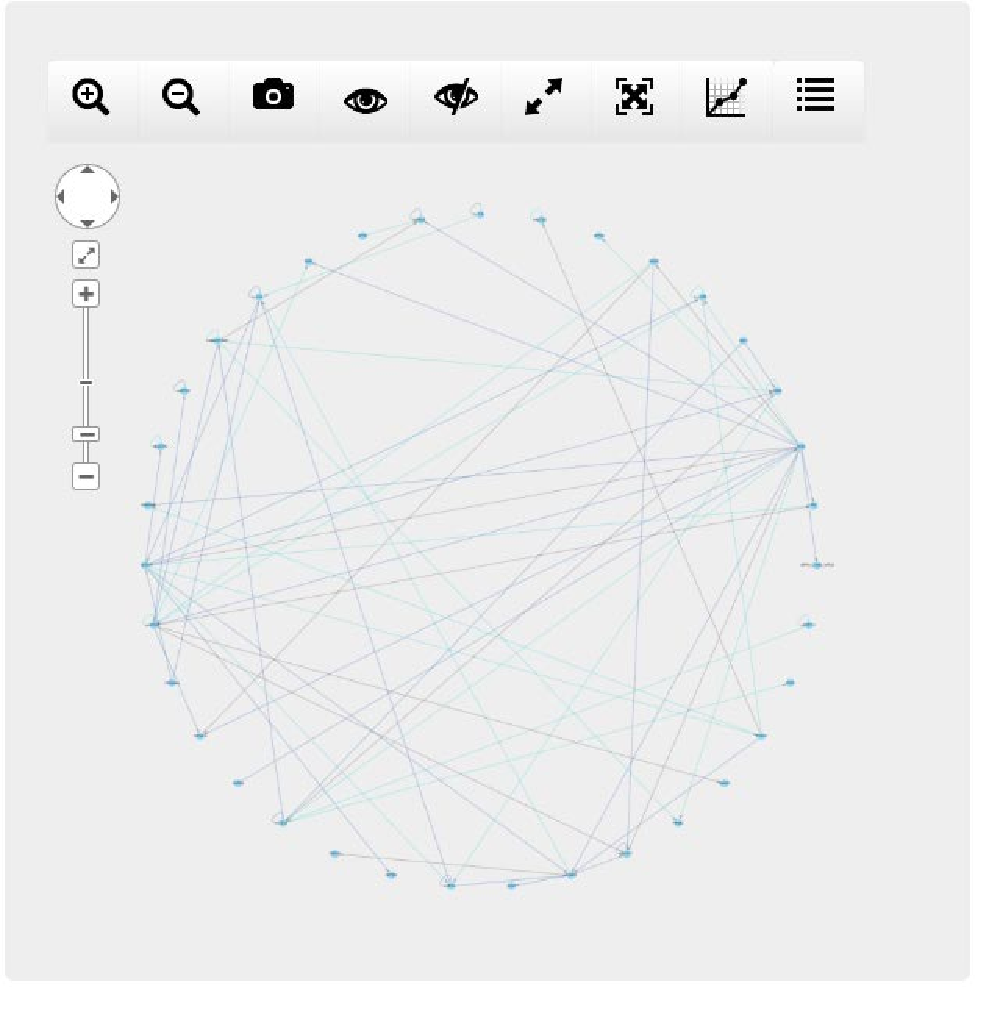
\includegraphics[width=0.3\textwidth]{l3}}}
      \subfigure{\label{juti4}}\addtocounter{subfigure}{-2}
      \subfigure{\subfigure[中心性布局]{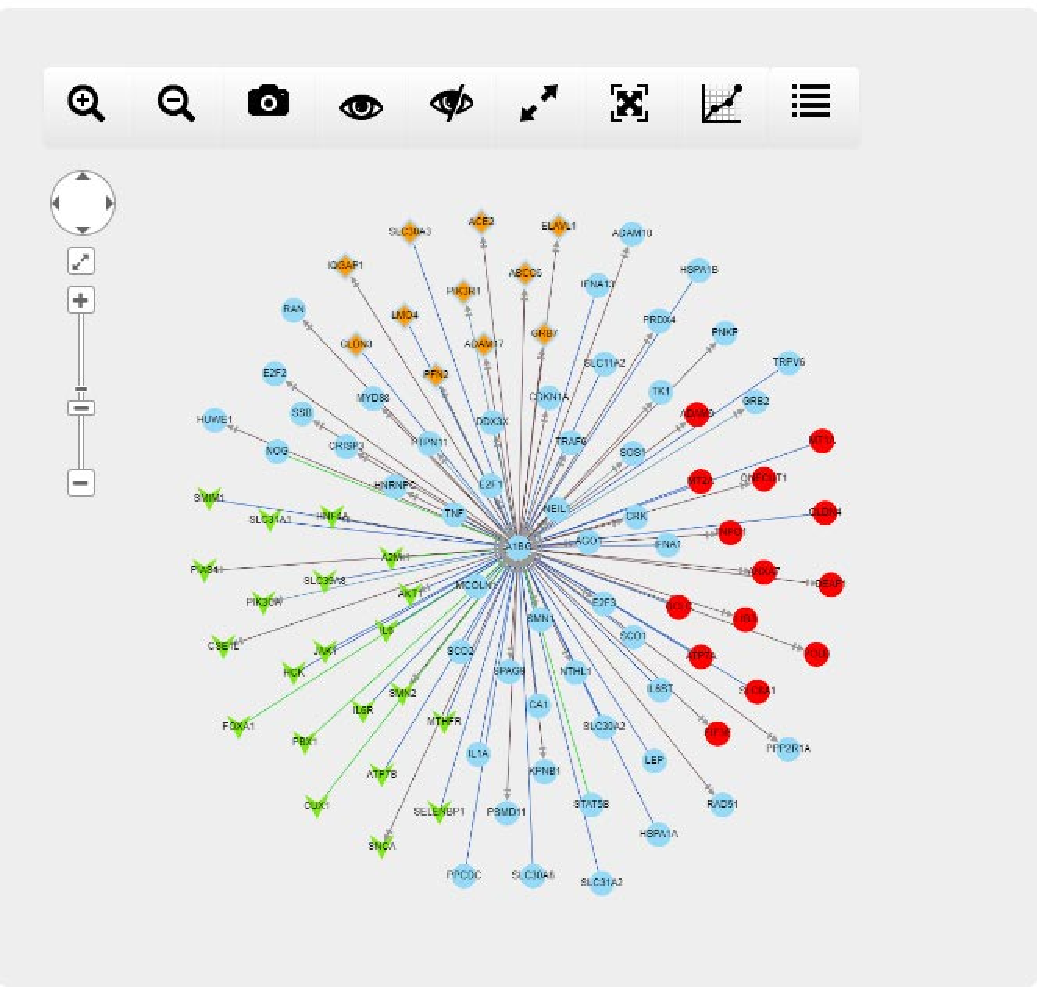
\includegraphics[width=0.3\textwidth]{l4}}}
      \subfigure{\label{juti5}}\addtocounter{subfigure}{-2}
      \subfigure{\subfigure[广度优先布局]{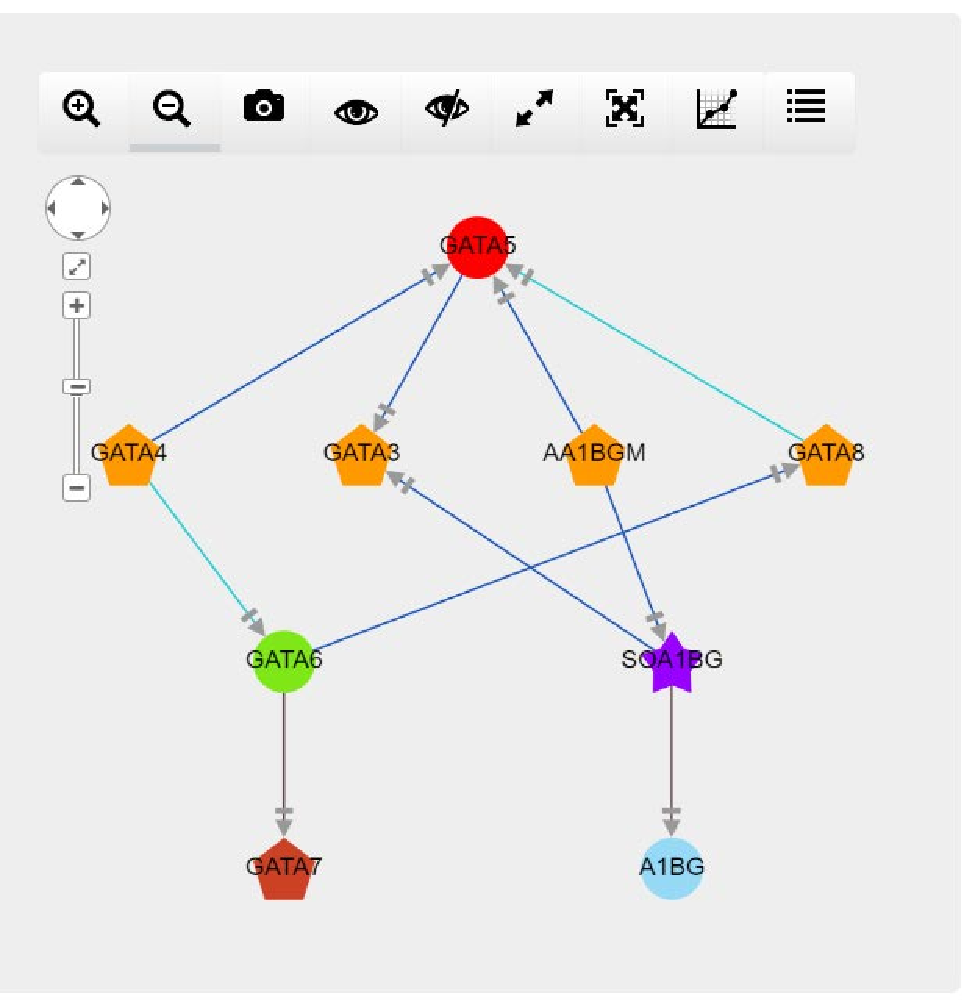
\includegraphics[width=0.3\textwidth]{l5}}}
      \subfigure{\label{juti6}}\addtocounter{subfigure}{-2}
      \subfigure{\subfigure[Cose布局]{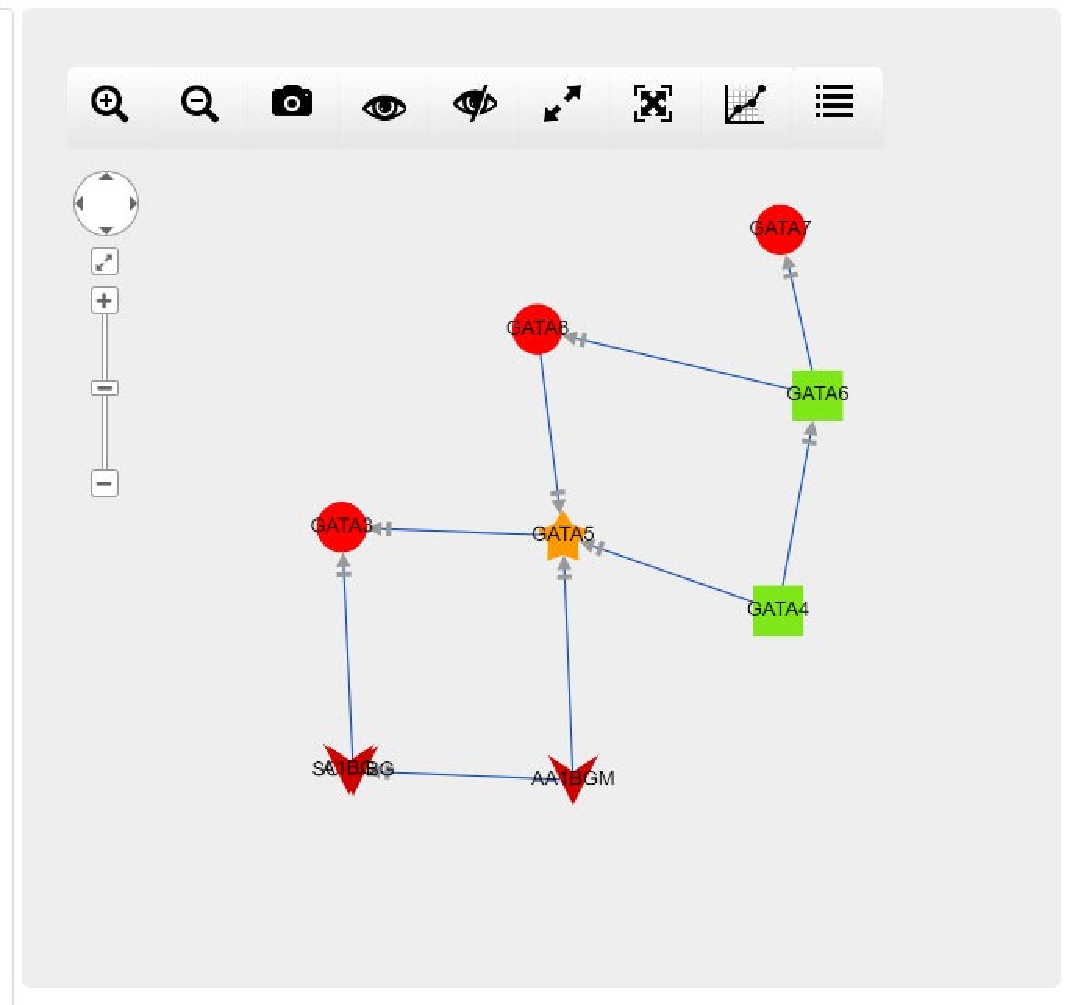
\includegraphics[width=0.3\textwidth]{l6}}}
      \subfigure{\subfigure[分散布局]{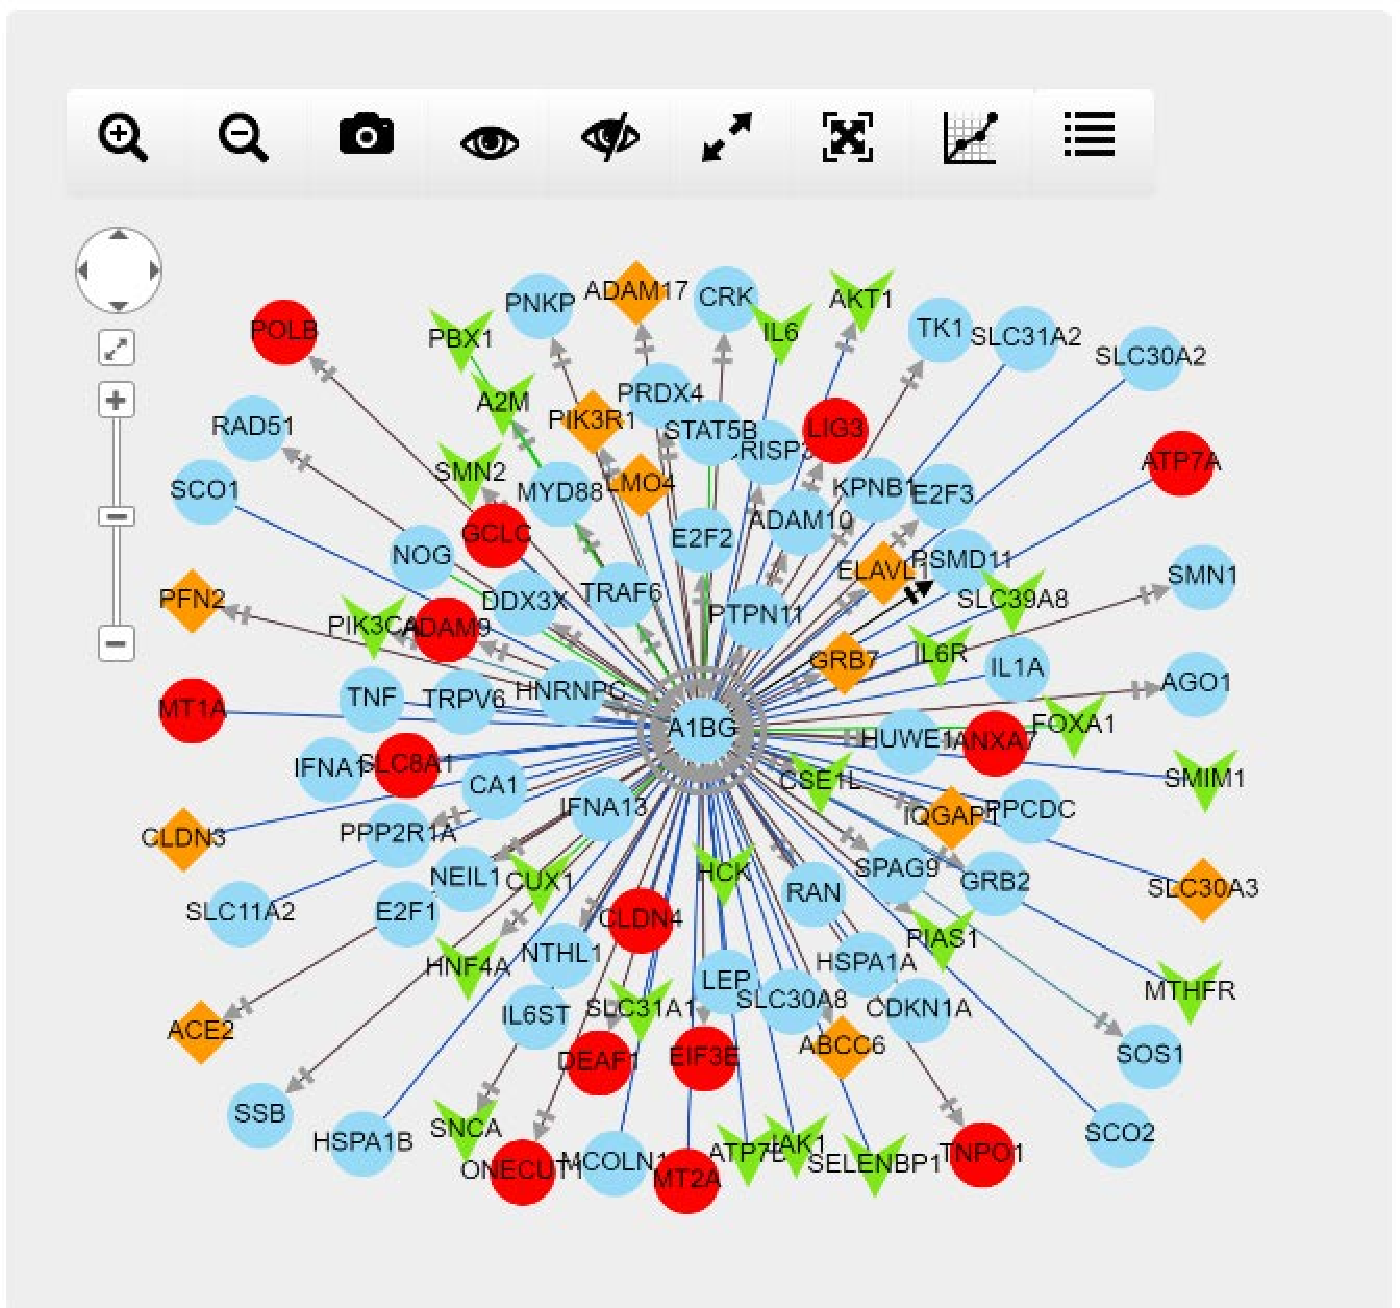
\includegraphics[width=0.3\textwidth]{l7}}}
      \subfigure{\label{juti5}}\addtocounter{subfigure}{-2}
      \subfigure{\subfigure[Dagre布局]{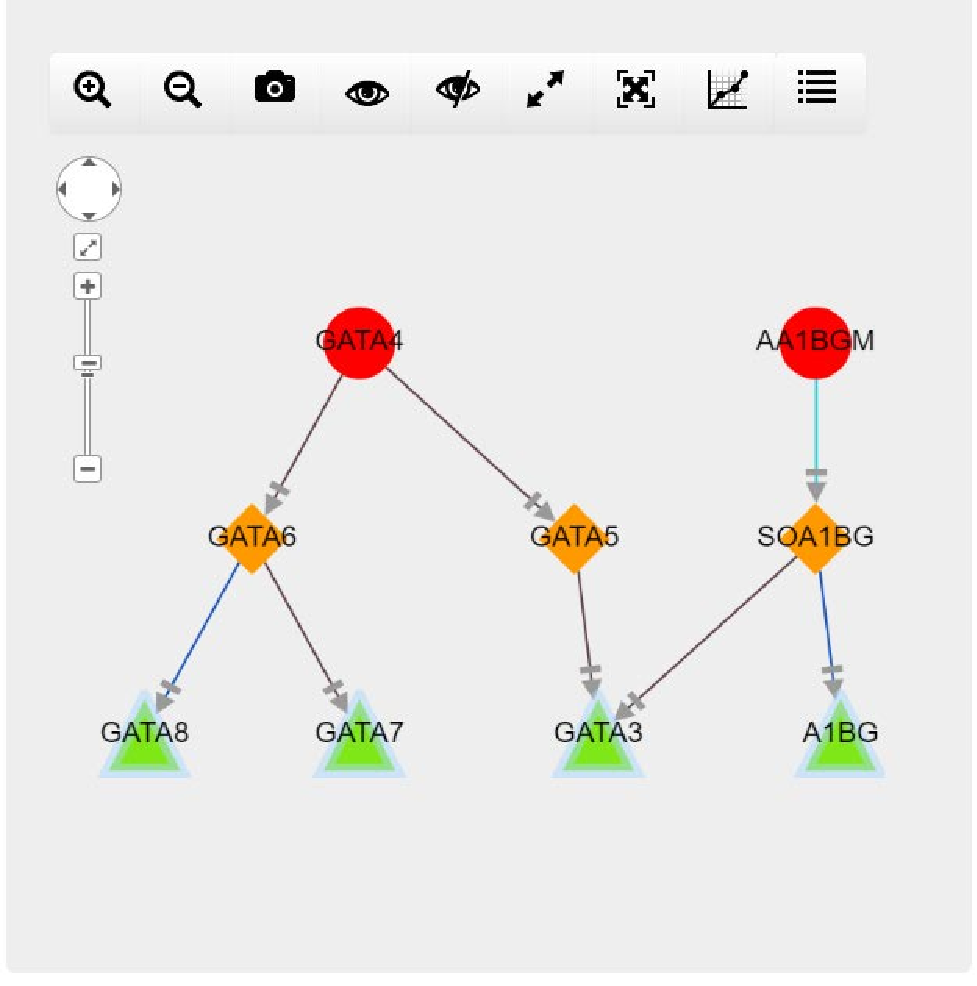
\includegraphics[width=0.3\textwidth]{l8}}}
      \subfigure{\label{juti6}}\addtocounter{subfigure}{-2}
      \subfigure{\subfigure[Arbor布局]{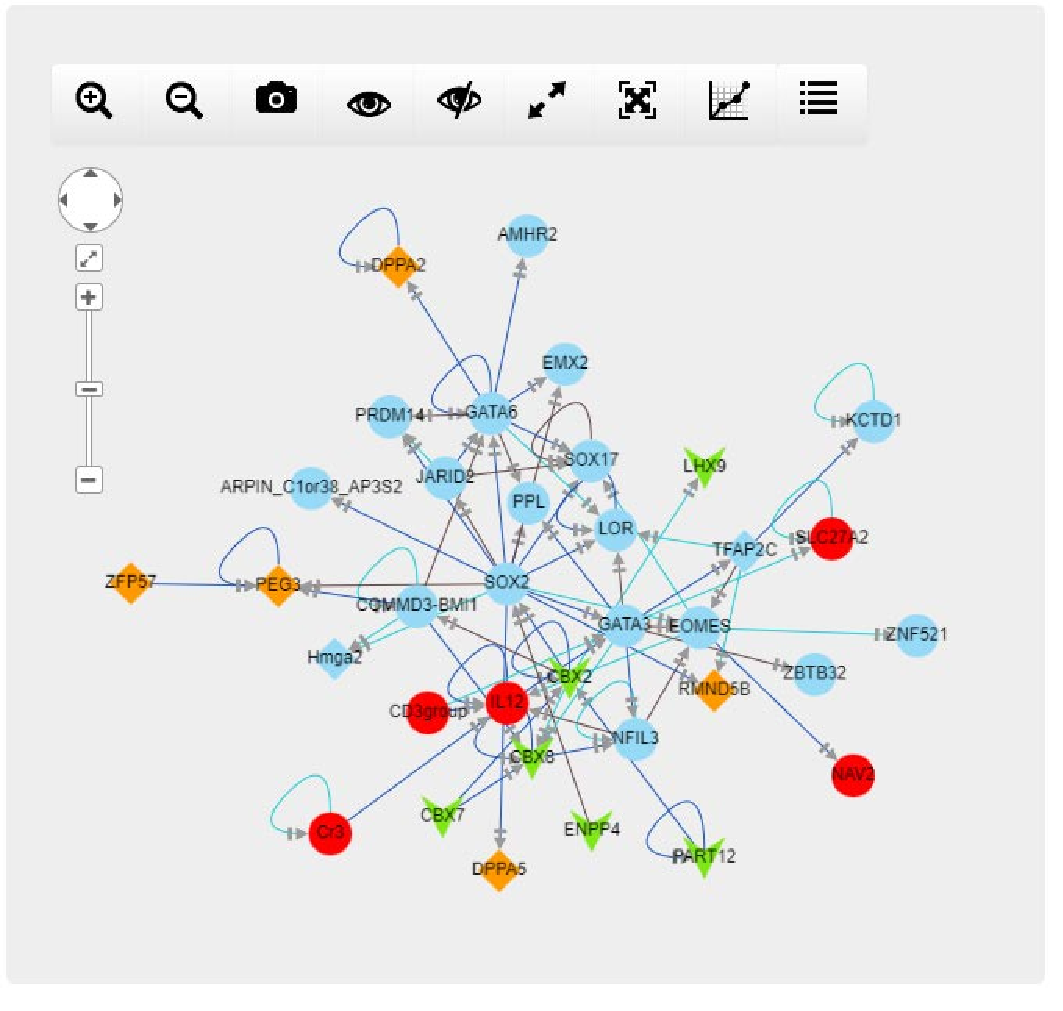
\includegraphics[width=0.3\textwidth]{l9}}}
    \end{minipage}
	\caption[layout]{本系统提供的9种布局}
	\label{layout}
  \end{minipage}
\end{figure}


\subsection{概要信息展示模块}
\begin{figure}[h]
  \centering
  \begin{minipage}{.95\linewidth}
    \setlength{\subfigcapskip}{-1bp}
    \centering
    \begin{minipage}{\textwidth}
      \centering
      \subfigure{\label{gaiyao1}}\addtocounter{subfigure}{-2}
      \subfigure{\subfigure[节点概要信息]{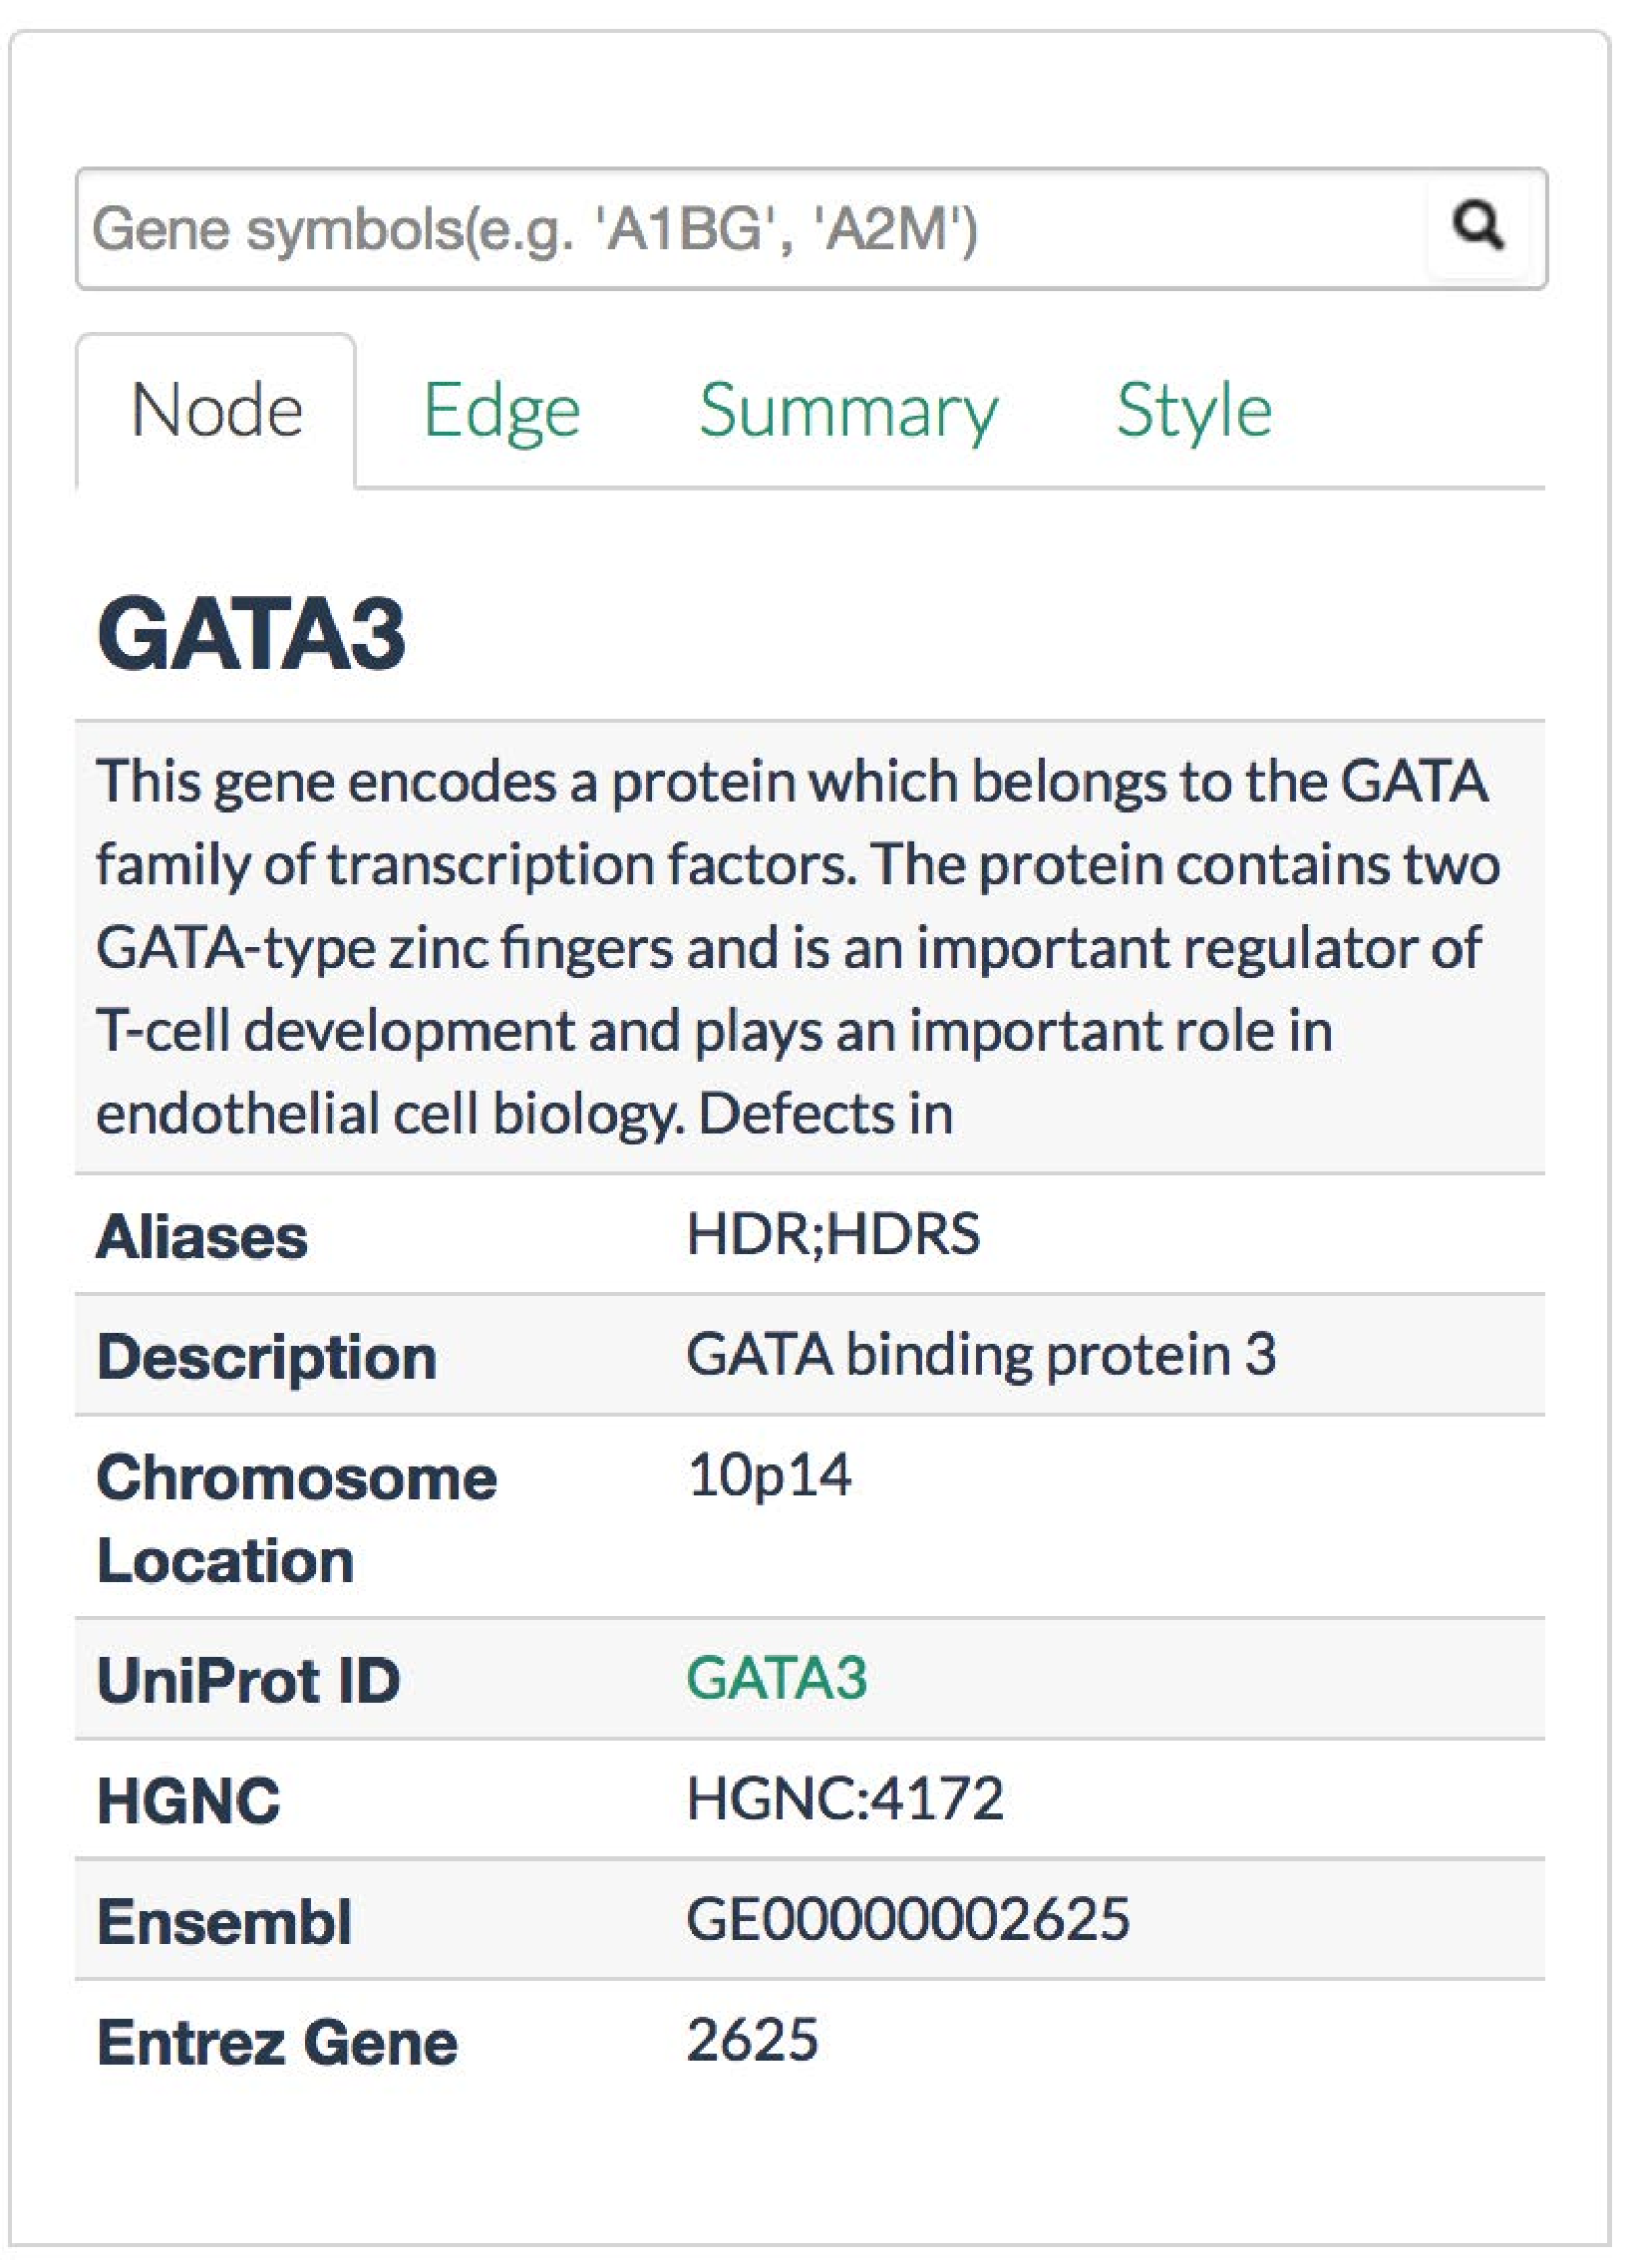
\includegraphics[width=0.2\textwidth]{tab1}}}
      \subfigure{\label{gaiyao2}}\addtocounter{subfigure}{-2}
      \subfigure{\subfigure[边概要信息]{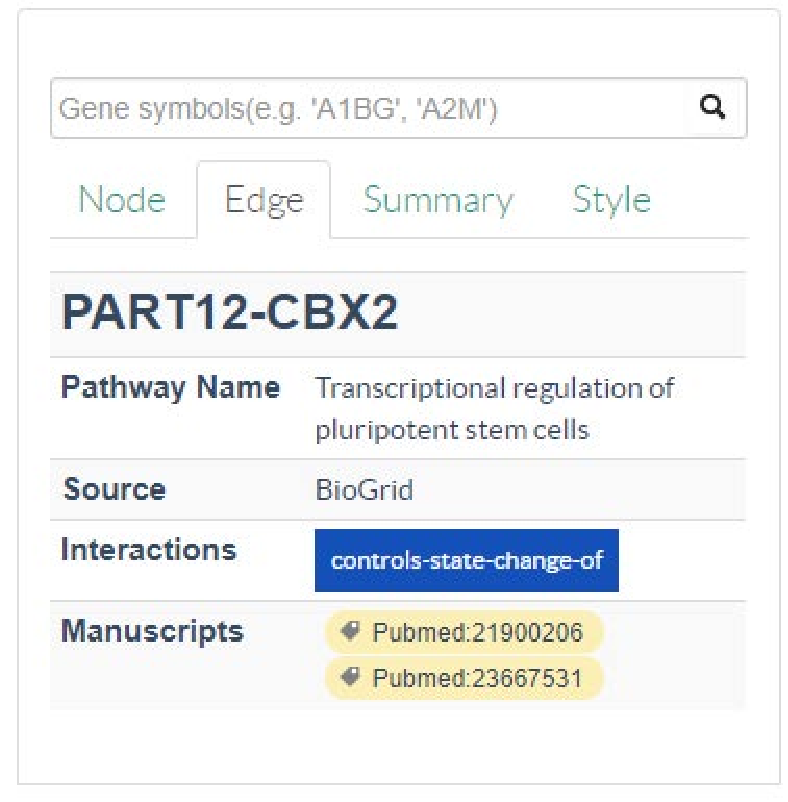
\includegraphics[width=0.2\textwidth]{tab2}}}
      \subfigure{\label{gaiyao3}}\addtocounter{subfigure}{-2}
      \subfigure{\subfigure[网络信息统计]{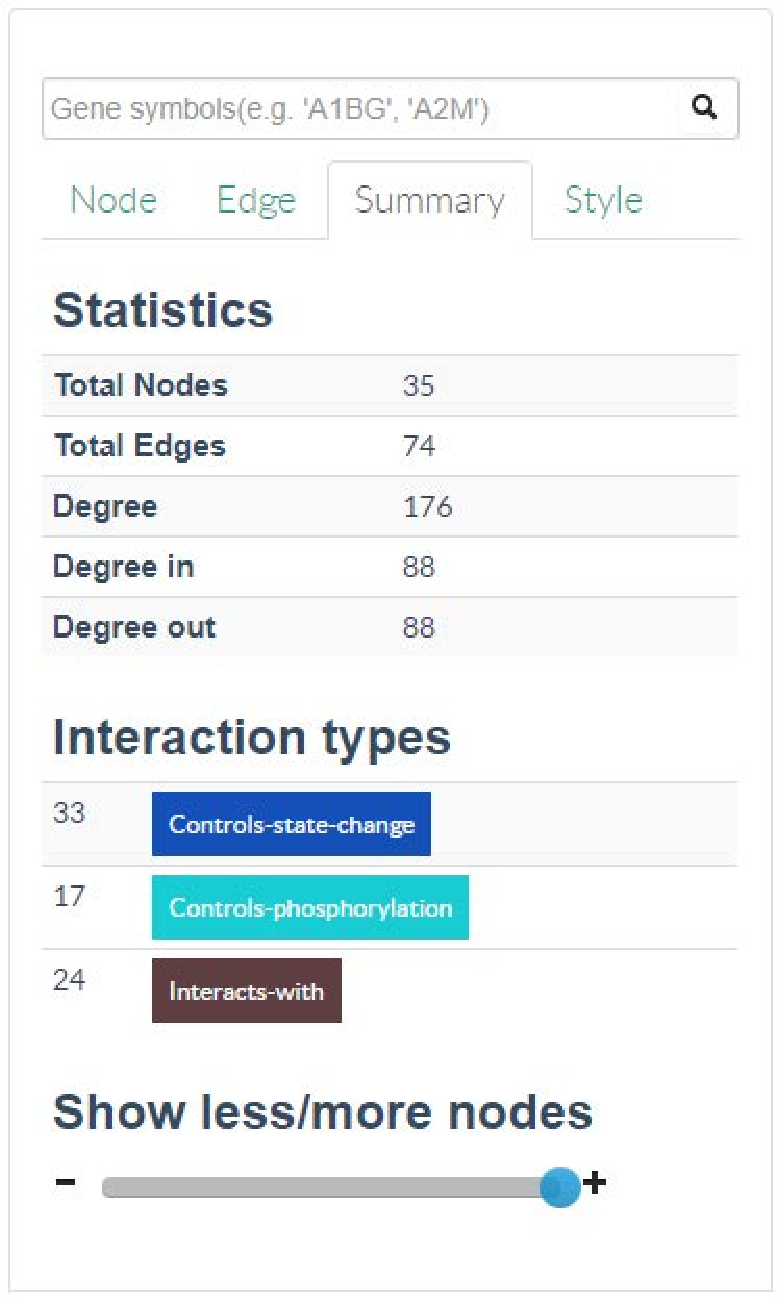
\includegraphics[width=0.2\textwidth]{tab3}}}
      \subfigure{\label{gaiyao4}}\addtocounter{subfigure}{-2}
      \subfigure{\subfigure[网络编辑模块]{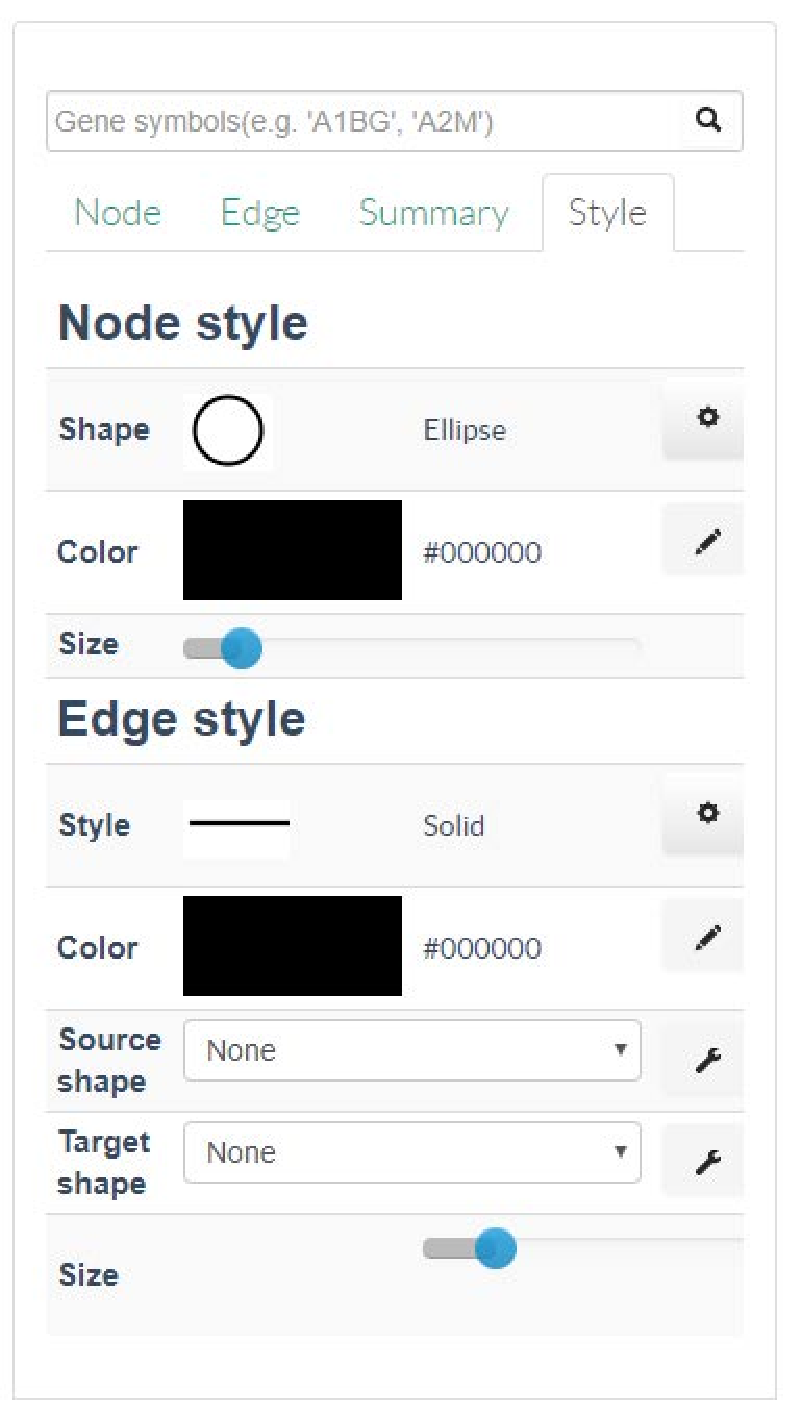
\includegraphics[width=0.2\textwidth]{tab4}}}
    \end{minipage}
	\caption[gaiyao]{概要信息展示模块对应的界面}
	\label{gaiyao}
  \end{minipage}
\end{figure}

概要信息展示模块分为四个子模块:节点概要信息、边概要信息、网络信息统计、网络编辑模块(如图\ref{gaiyao})。各子模块功能如下:

如上文所介绍本系统中生物通路网络默认的节点是基因,当用户点击某个节点时,节点概要信息模块如图\ref{gaiyao1}会列出对该节点信息摘要描述信息(通常为一段文字),该基因的别名、位置信息、UniProt\cite{}数据库中的编号信息、HGNC\cite{}数据库中的编号信息、Ensembl\cite{}数据库中的编号信息,基因编码信息。当有些基因在部分数据库中不存在编号时,系统会给出缺省值'-'。(如图\ref{gaiyao1})

当用户点击某个边时,边的概要信息模块会列出该边(相互作用)所在的生物通路名,该边(相互作用)的数据来源、该边的类型和该边相关联的文献编号。 为区分网络中不同的边的类型,边的作用类型在该模块以不同色块形式给出,每一类使用一个颜色码,该颜色码和生物通路网络中该边的颜色一致。与该边相关的文献编号以标签卡的形式给出,当用户点击该标签卡时系统会跳转到该文献来源的页面。(如图\ref{gaiyao2})

当用户使用框选功能选中网络中的子网(一部分节点和边时),网络信息统计模块,会给出该子网中包含的节点数量、边数量、子网络中所有节点度的总和、子网络中所有节点出度的总和、子网络中所有节点入度的总和。子网中各种类型边信息也会被统计出来。系统默认状态下统计整个生物网络的信息。(如图\ref{gaiyao3})

当用户想修改网络中某些元素(节点或边)的信息时。网络编辑模块提供节点和边信息的修改功能。用户可以修改节点的形状(共11种)、节点的颜色、节点的大小。为提升用户的体验,当修改颜色时系统为用户提供了拾色器功能,用户可以方便的选择自己喜欢的颜色信息。节点大小的修改可以通过滑块拖动的形式实现。(如图\ref{gaiyao4})

\subsection{详细信息展示模块}
详细信息展示模块:基因详细信息展示、疾病详细信息展示、药物信息展示、通路信息展示、网络分析结果展示、基因表达信息展示模块如图\ref{juti}所示。各子模块的功能如下:

当用户点击某个节点时,基因详细信息展示模块列出与选中节点相关联基因的详细信息。这部分信息包含节点概要信息模块展示的信息,此外还包含基因的编码信息、基因的注释信息、基因的相关文献信息如图\ref{juti1}所示。

当用户点击某个节点时,疾病详细信息展示模块列出与选中节点相关联疾病的详细信息。疾病详细信息包括与节点相关的疾病数量信息、
疾病数据来源信息(以标签卡形式给出),疾病的名称信息如图\ref{juti2}所示。

当用户点击某个节点时,药物详细信息展示模块列出与选中节点相关联药物的详细信息。药物详细信息包括与节点相关的药物数量信息
,药物数据来源信息(以标签卡形式给出),药物的名称信息如图\ref{juti3}所示。

当用户点击某个节点时,通路信息展示列出与选中节点相关联通路的详细信息。通路详细信息包括与节点相关的通路数量信息
,通路名称信息、通路中包含的基因数量、通路与选中节点之间的关联得分,该得分是来自GeneCard\footnote{}官方提供数据如图\ref{juti4}所示。

当用户点击某个节点时,网络分析结果展示模块会给出选中节点在网络中度、度的中心性、密集中心性、介数中心性的数值。同时在网络可视化模块,我们提供了网络分析按钮,当用户点击这个按钮时,分析结果会在该模块以柱状统计图的形式给出,分析包括度分布、最短路径分布等如图\ref{j5}所示。

当用户点击某个节点时,与选中节点相关的基因表达信息会在基因表达信息展示模块给出。表达信息包括该基因在GXTEX\cite{}、 ILITA\cite{}、GEOPS\cite{}和CGAP SAGE\cite{}中的表达情况如图\ref{j6}所示。

\begin{figure}[h]{\label{juti}}
  \centering
  \begin{minipage}{1.0\linewidth}
    \setlength{\subfigcapskip}{-1bp}
    \centering
    \begin{minipage}{\textwidth}
      \centering
      \subfigure{\label{juti1}}\addtocounter{subfigure}{-2}
      \subfigure{\subfigure[基因详细信息]{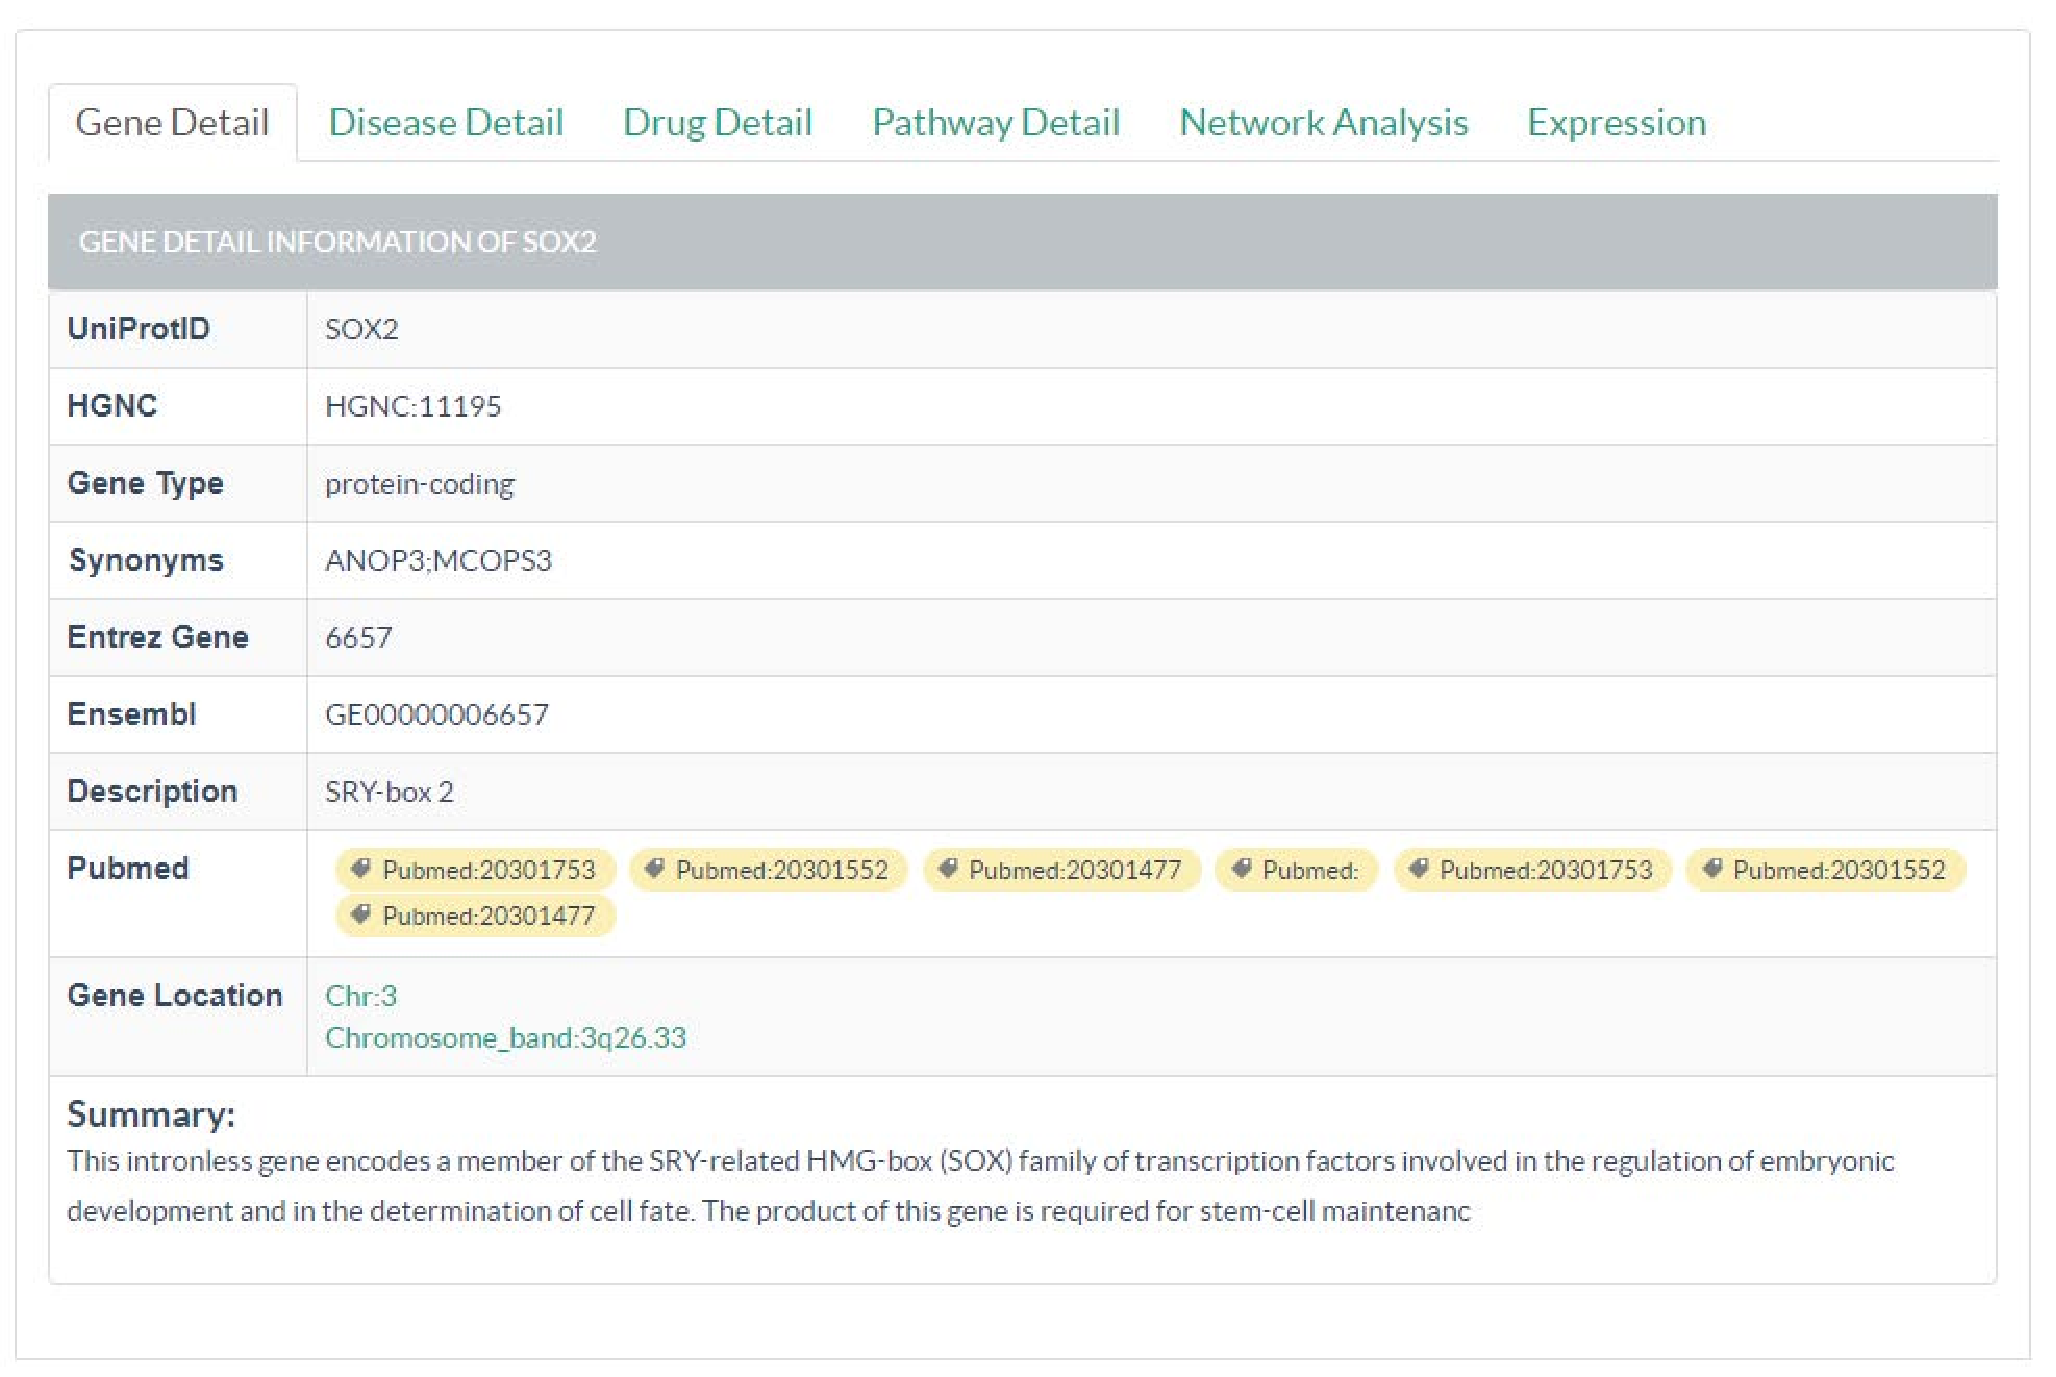
\includegraphics[width=0.4\textwidth]{juti1}}}
      \subfigure{\label{juti2}}\addtocounter{subfigure}{-2}
      \subfigure{\subfigure[疾病详细信息]{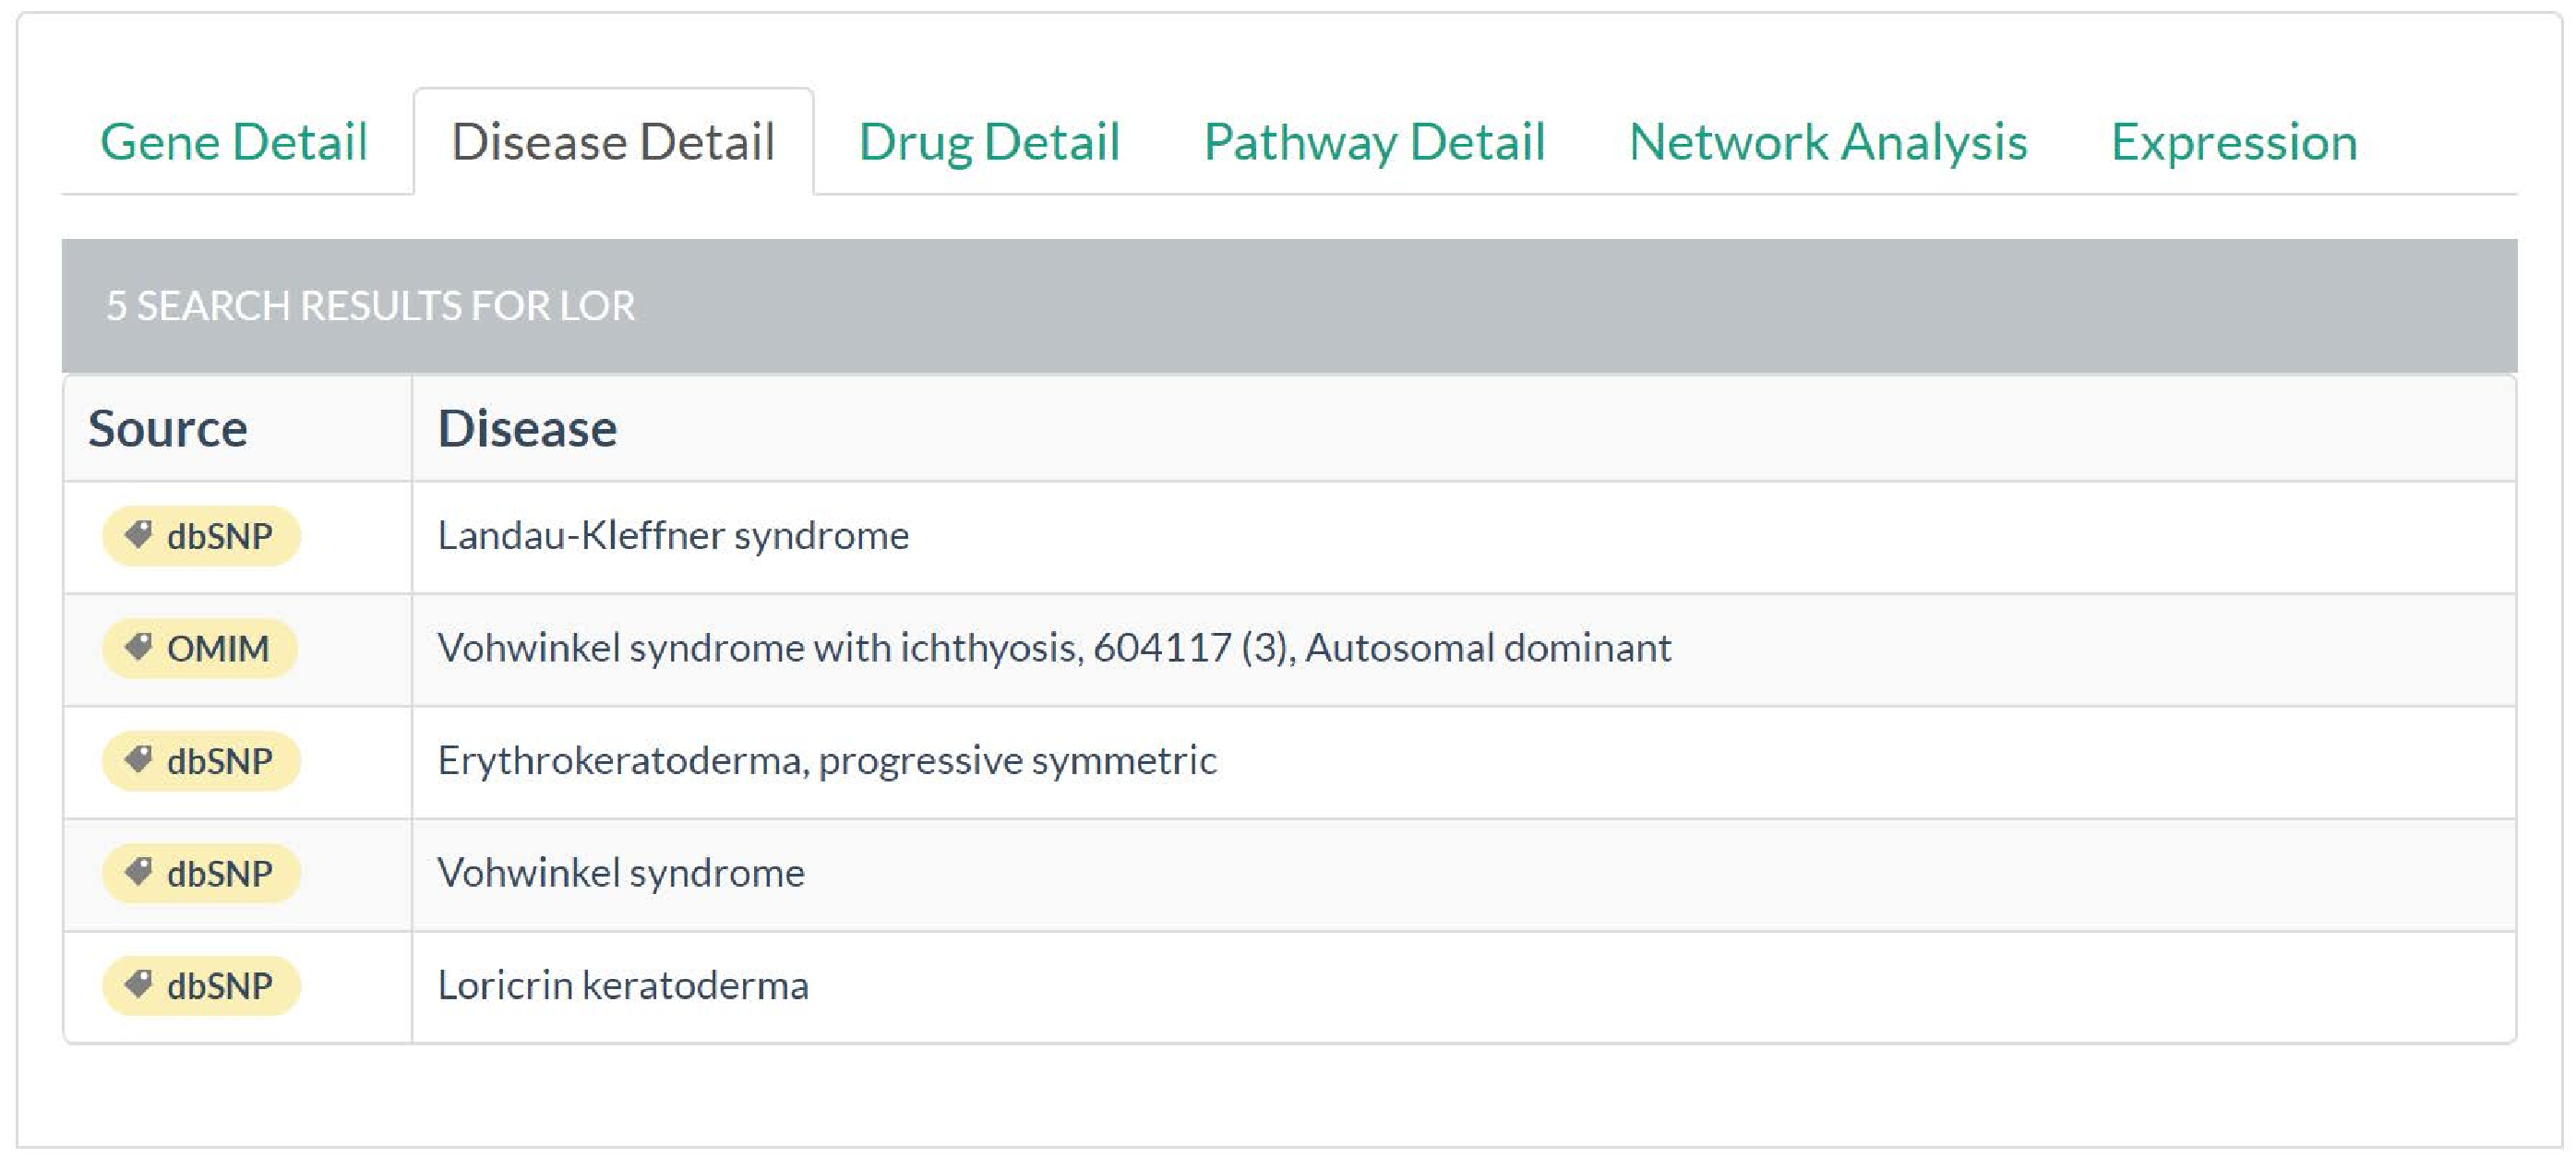
\includegraphics[width=0.4\textwidth]{juti2}}}
      \subfigure{\label{juti3}}\addtocounter{subfigure}{-2}
      \subfigure{\subfigure[药物详细信息]{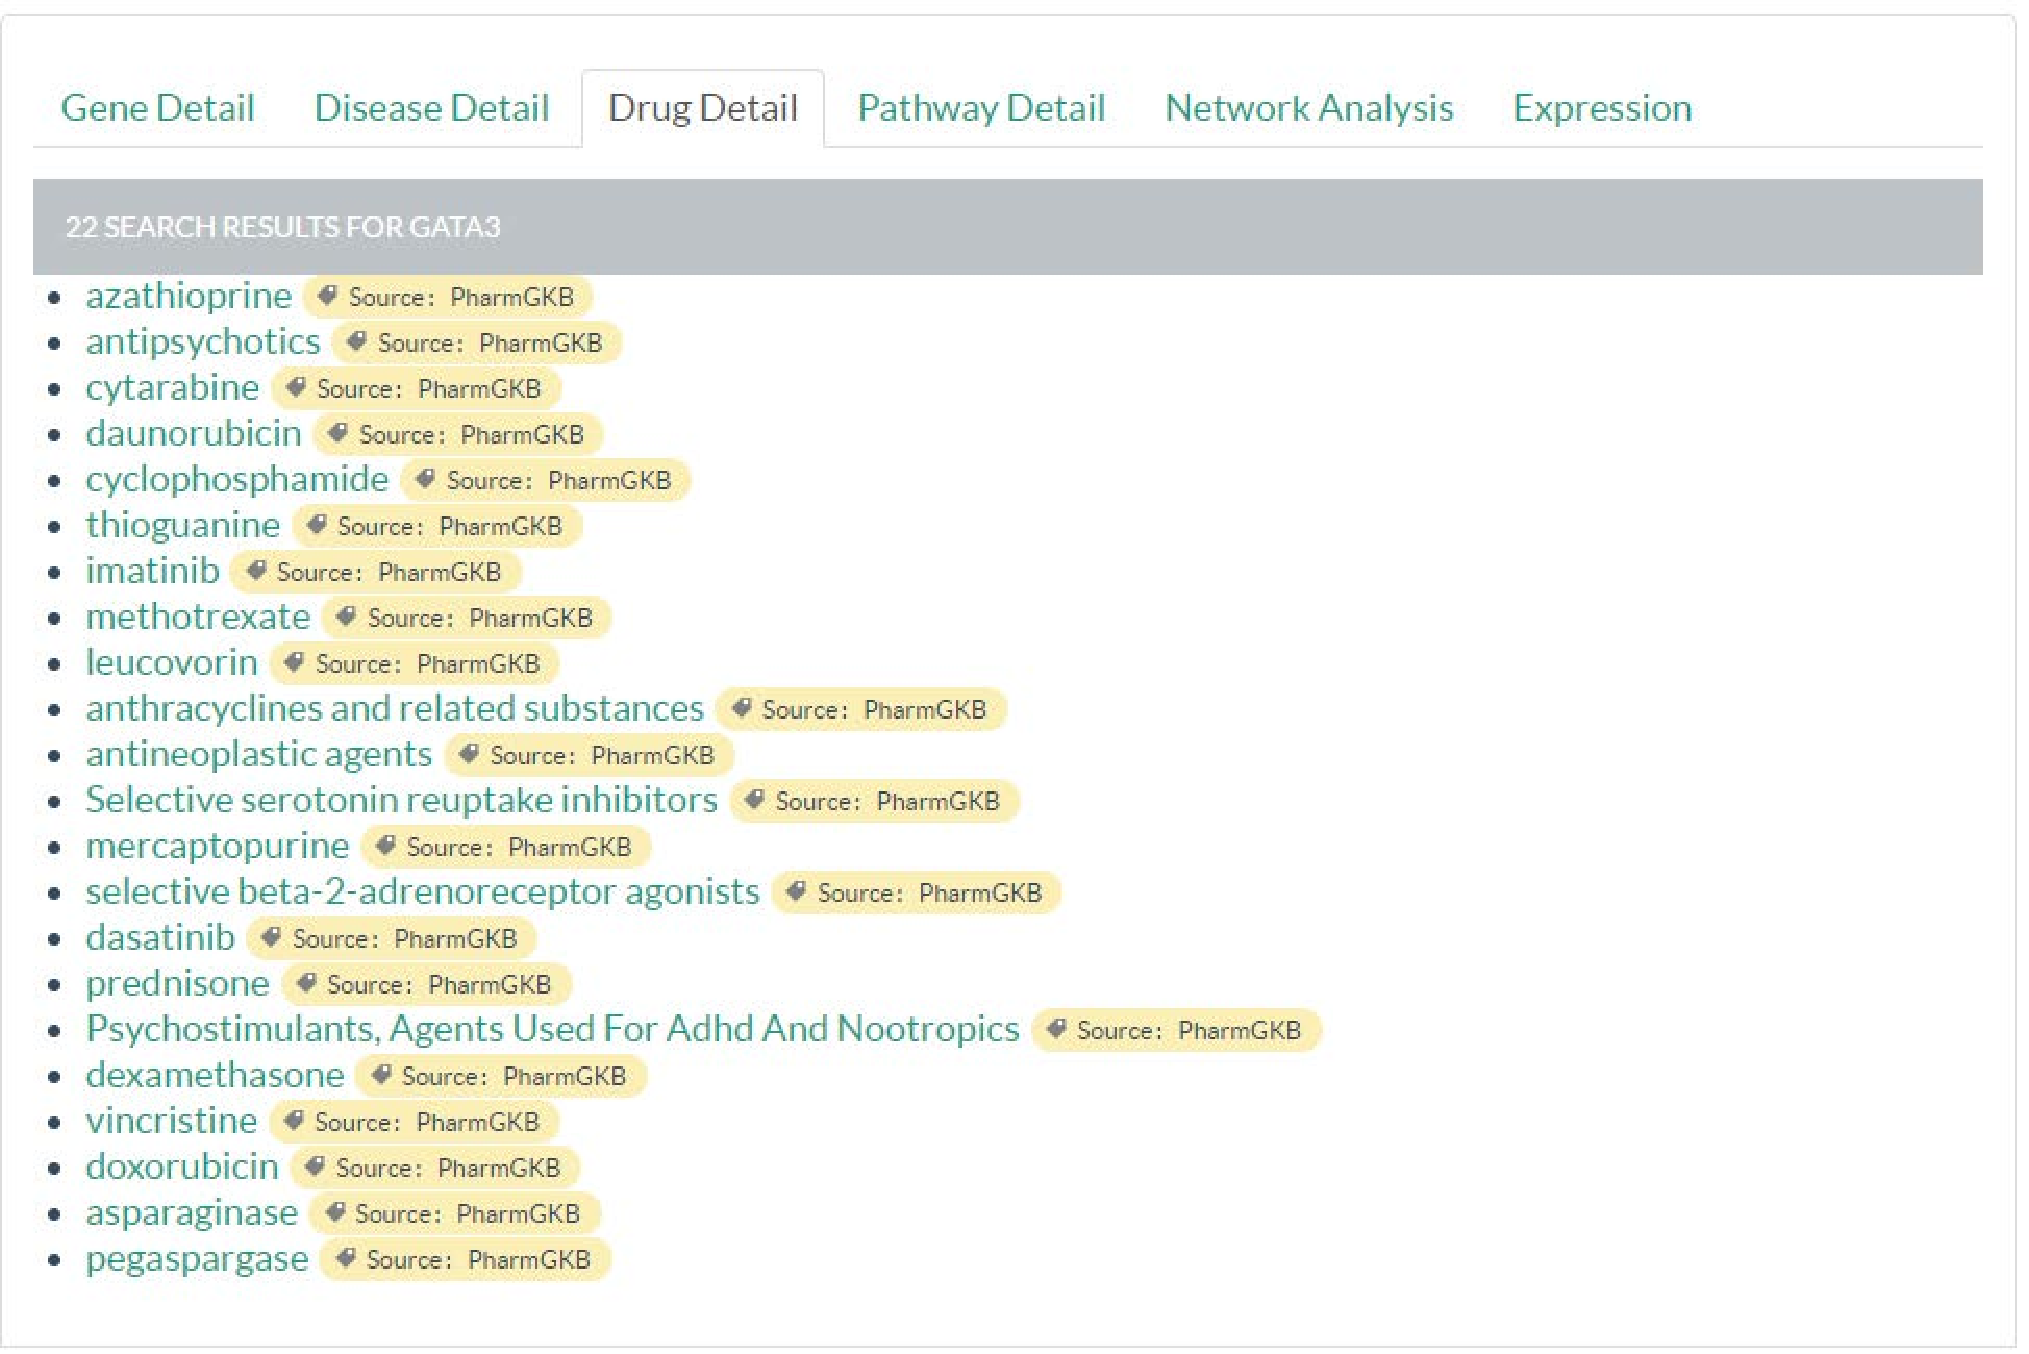
\includegraphics[width=0.4\textwidth]{juti3}}}
      \subfigure{\label{juti4}}\addtocounter{subfigure}{-2}
      \subfigure{\subfigure[通路详细信息]{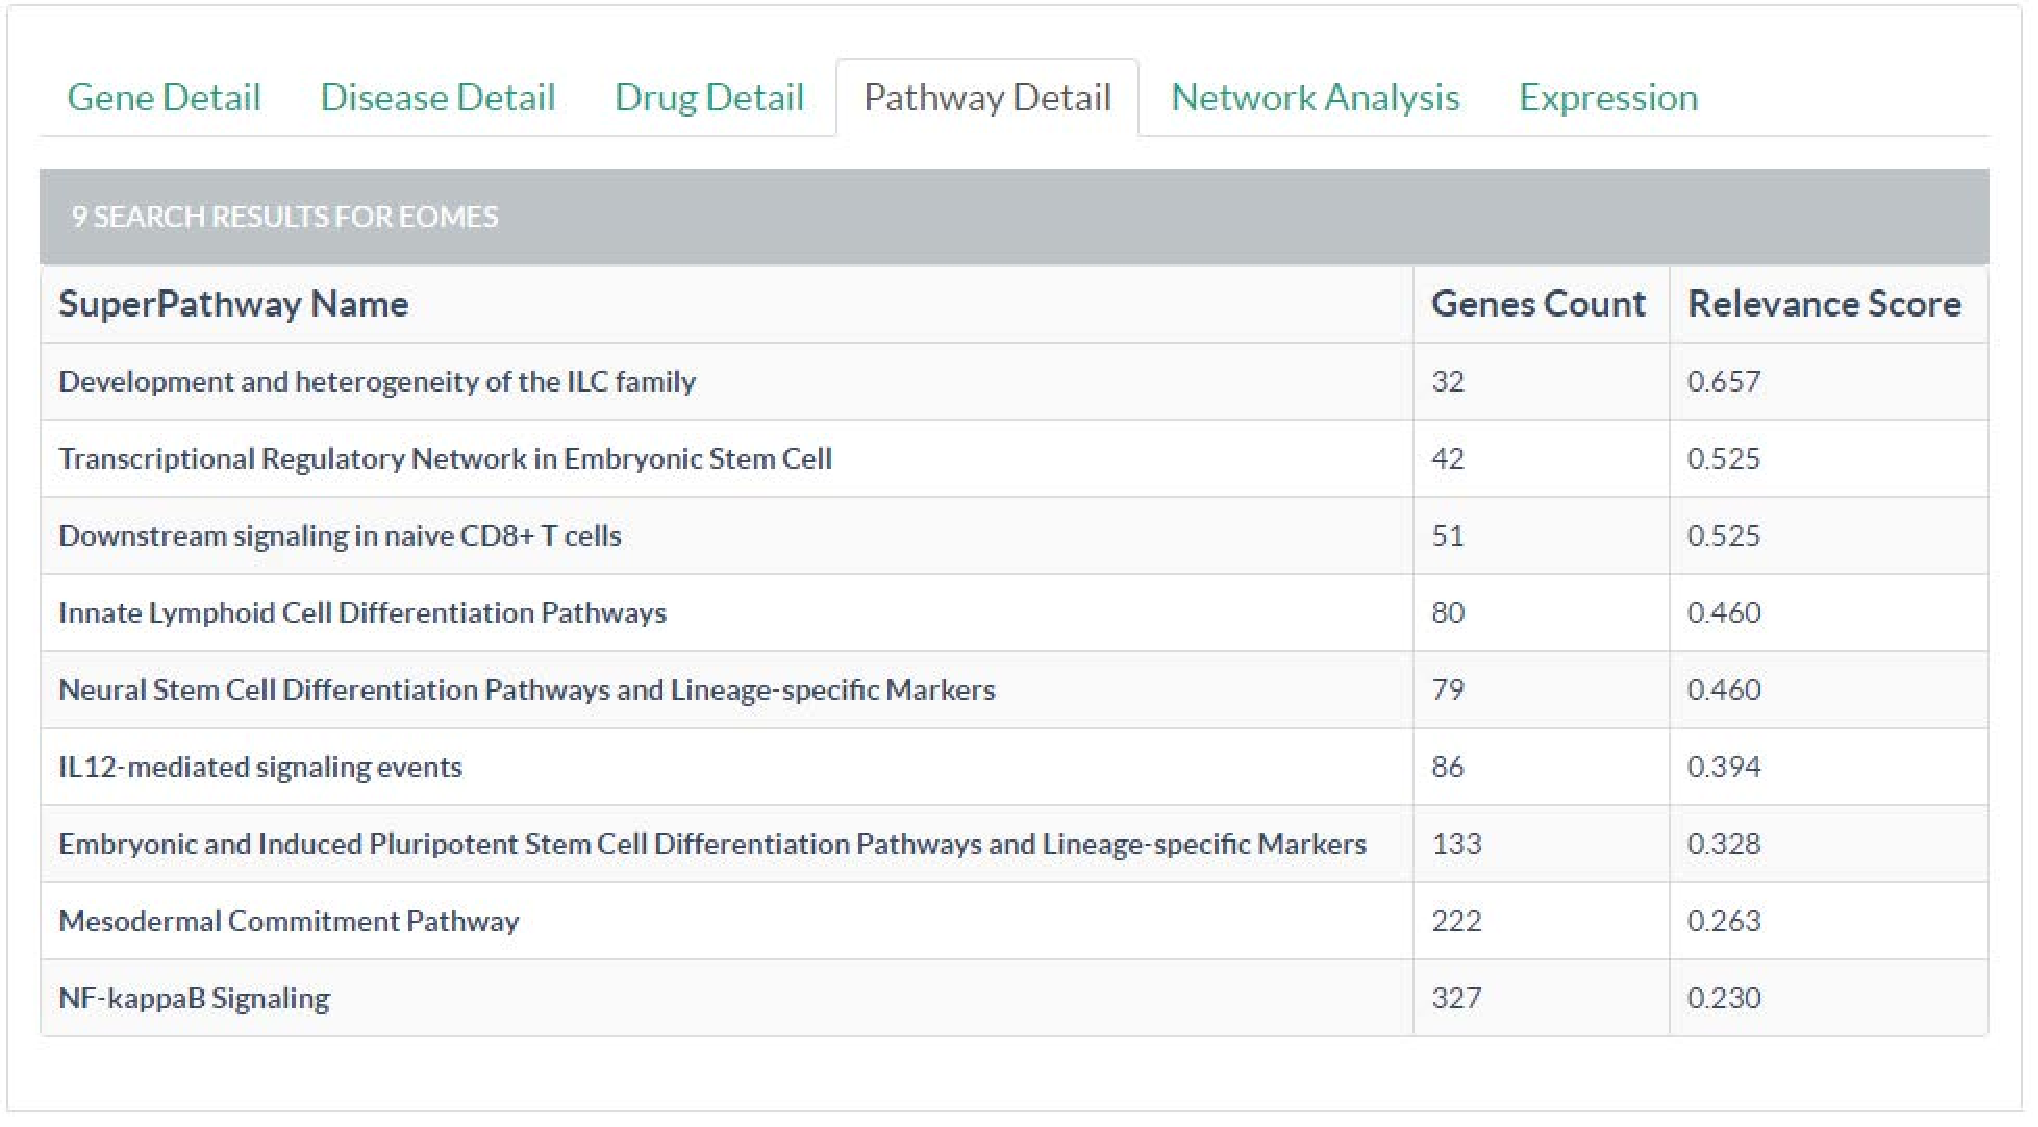
\includegraphics[width=0.4\textwidth]{juti4}}}
      \subfigure{\label{j5}}\addtocounter{subfigure}{-2}
      \subfigure{\subfigure[网络分析信息]{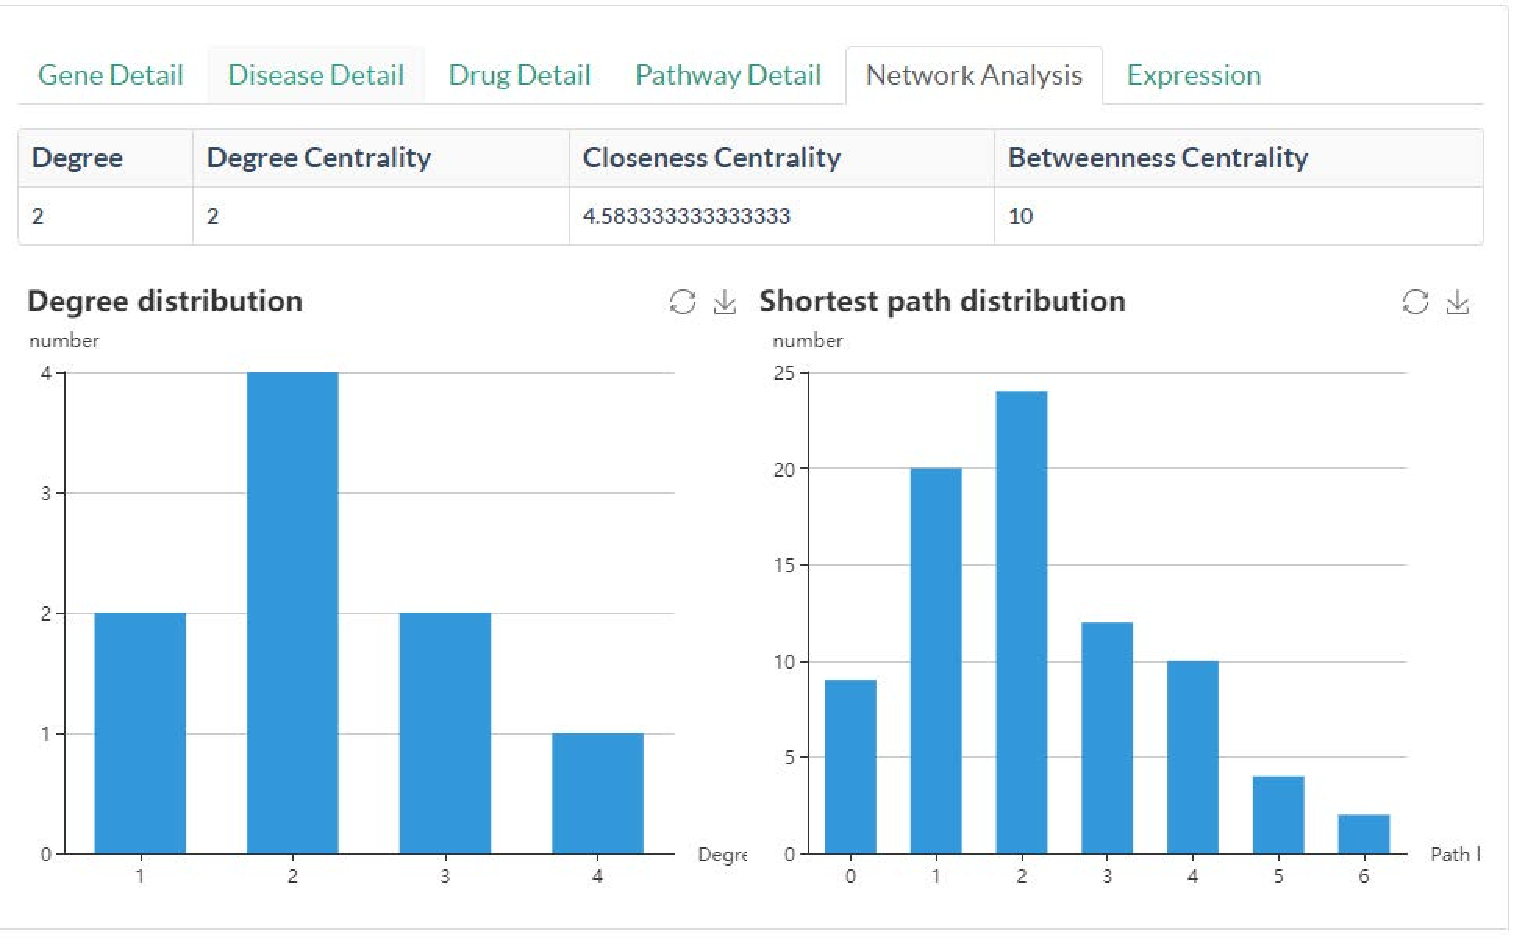
\includegraphics[width=0.4\textwidth]{juti5}}}
      \subfigure{\label{j6}}\addtocounter{subfigure}{-2}
      \subfigure{\subfigure[基因表达信息]{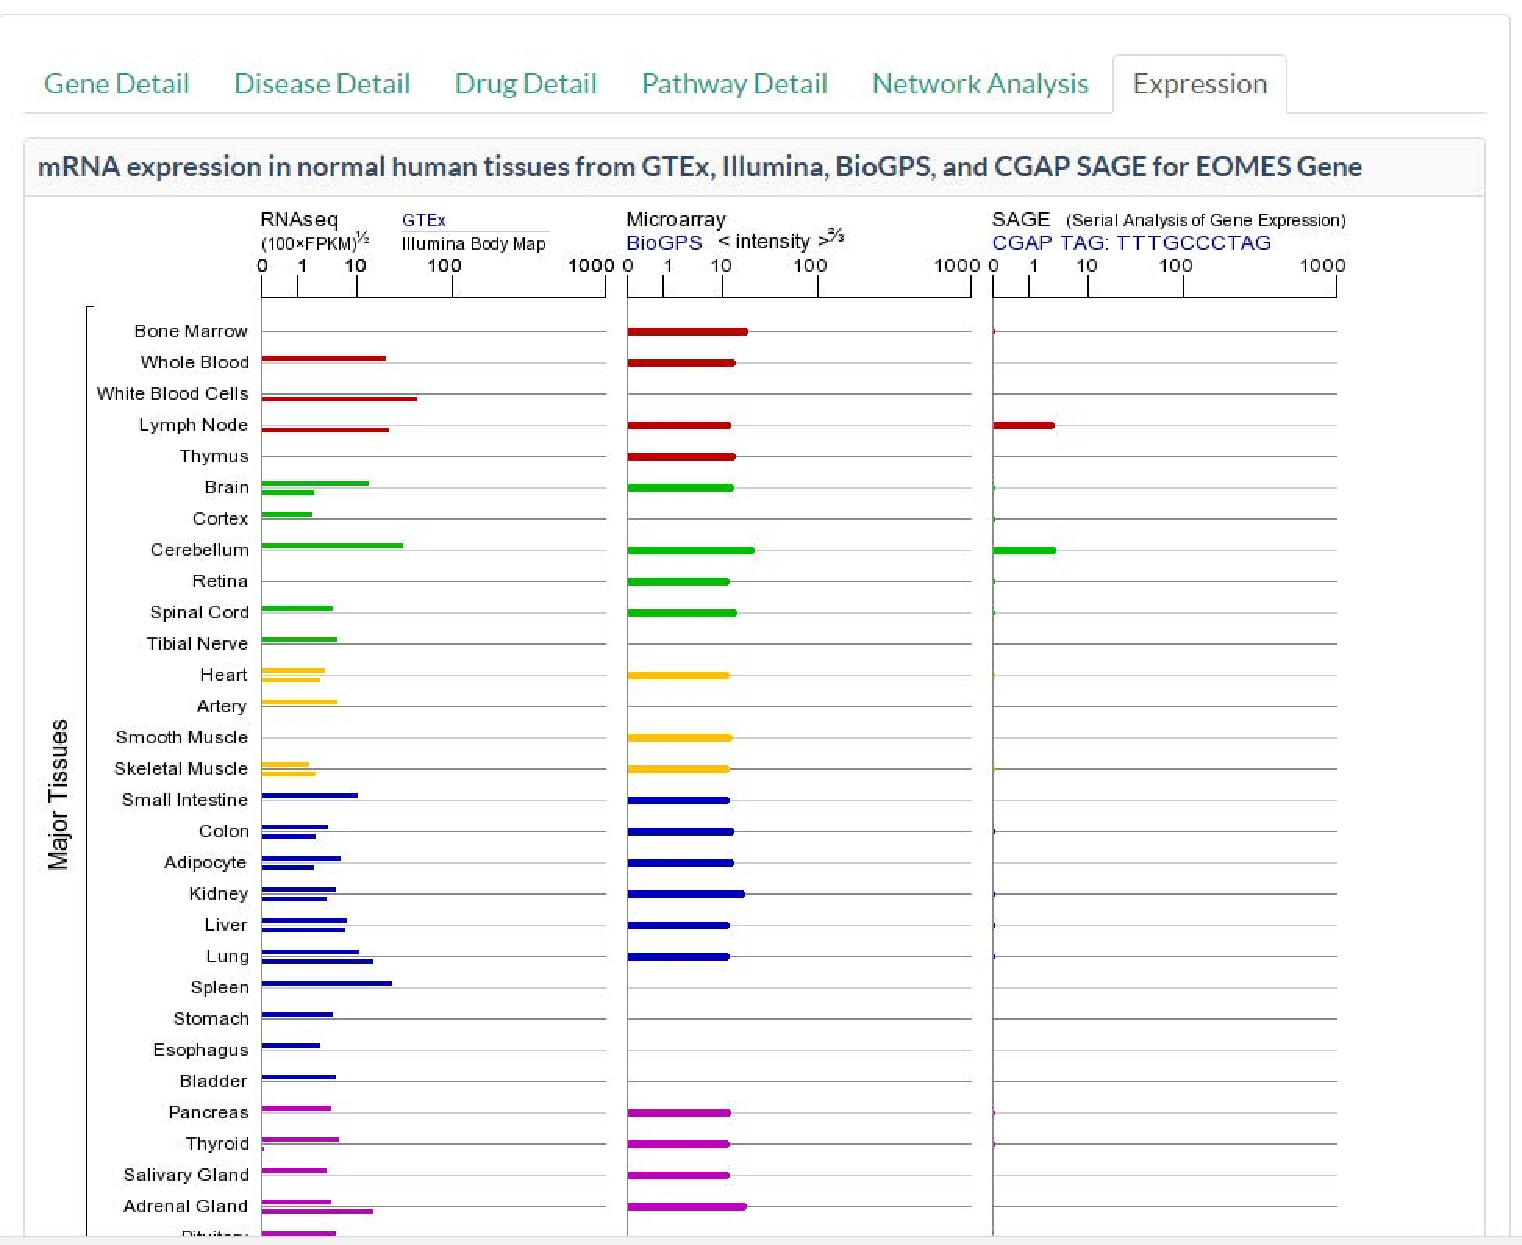
\includegraphics[width=0.4\textwidth]{juti6}}}
    \end{minipage}
	\caption[juti]{详细信息展示模块对应的界面}
	\label{juti}
  \end{minipage}
\end{figure}



\section{系统实现技术}
为了搭建了一个高效、实用、易于维护的通路网络可视化平台,本系统采用了如下的技术:

\subsection{开发语言}
后台开发语言:本系统的后台开发语言使用了Python语言,随着人工智能技术的研究日益深入,Python语言成为了很多开发者的首选。Python语言简洁而强大。其优势在于Python相对于C++、Java等语法简单清晰,表述相同的概念和功能其代码量更小。Python语言是提供了多种的编程范式,面向对象、函数式编程均被Python所支持。Python用于数据处理、科学计算、制图等,该语言可以使用丰富的第三方模块。和昂贵的Matlab软件相比Python 是免费的,Python可以实现向量数组等运算同时也支持绘图功能。Python语言是和平台无关的语言,支持多种操作系统,Python代码可以被打包运行到各种流行的操作系统上。Python语言提供各种工具可以帮助使用者更好的分析和解决问题,对于使用者Python的语法简单易懂可读性好,使用者可以根据自己的需求去编制自己的程序包对该语言进行扩展,可以有效帮助使用者完成科研工作。Python在Web开发领域也日益强大多种web框架如Django、Flask、Tornado等。Python可以集web开发、数据分析、数据可视化、数据库开发为一体,适合本系统的需求,因此作为了本系统后台的开发语言。

前端开发语言:本系统的前端采用了html5+CSS+JavaScript。随着互联网技术的日益发展,2013年随着第五代html标准的提出,互联网前端开发技术开启了崭新的时代,大量web应用使用html5技术更新了其前端,html5开源社区也日益壮大,html5成为了web前端开发主流的语言.CSS是一种网页静态修饰语言,它可是实现网页中元素的精确控制,对网页中个元素进行修饰描述,极大提升网页的用户体验。JavaScript(JS)也是一种在网页前端广泛使用的动态、解释性、弱类型的开发语言,最早被用于html的动态修饰,但是随着技术的发展,JS的解释器已经成为了浏览器自身的一部分,JS的功能日益壮大,在大数据时代,JS已经成为大数据可视化领域最有影响力的语言,基于JS语言的大量可视化库被开发出来如D3.js、Cytoscape、plotly.js等。

\subsection{技术框架}
在Web开发过程中,使用成熟的框架有利于提升开发的效率、提高应用的安全性和维护性,借助成熟的框架,可以实现前后端的分离,有利于进行团队开发,因此本系统中前端使用了基于JS的前端框架,后端使用了基于Python语言的后端框架:

前端框架:本系统前端使用了Bootstrap作为前端开发框架。其主要优势是在于响应式网页的设计。在实现用户界面时,Bootstrap语法简单明了,可以实现界面的快速迭代。

后端框架: 本系统后端使用了Tornado作为后端开发框架。Tornado是主流的Web服务器框架,其主要的有点是其非阻塞的特点,响应的速度很快,该框架可以每秒处理数以千计的连接。


\subsection{数据库技术}
本系统使用MySQL作为后台数据库,MySQL数据库是被广泛使用的关系型数据库,MySQL支持windows、Linux、FreeBSD等在内多种操作系统,与其他的数据库相比MySQL的主要优势在于:MySQL支持常见的规范的SQL语句;移植性好,可以跨平台使用;MySQL具有较好的执行效率,同时具有丰富的文档和技术支持社区; 支持图形化和命令行形式的管理工具,数据库管理、数据库查询优化简单方便。

为了保证数据库的访问高效、稳定。我们在本系统中使用了ORM技术,ORM是指对象-关系映射,ORM层实际上充当了数据库的中间件角色,主要解决了应用程序中的对象到关系数据库中数据的映射,解决了应用程序中的对象和关系数据库中的业务实体出现表现形式不同的问题,提高了数据库迁移的能力,提高了开发的效率、当数据库查询很复杂时,使用ORM可以优化查询语句,避免因数据库查询语句不当造成的性能问题。本系统中我们使用SQLAlchemy作为实现ORM的工具,SQLAlchemy为系统提供了良好的数据接口、便于引入缓存、对外隐藏了数据库提高系统的安全性。

\subsection{可视化技术}
本系统的可视化技术主要基于Cytoscape的应用编程接口,Cytoscape是一款强大的网络可视化软件,由于其强大的性能、出色的网络绘制能力,被广大的研究人员使用。Cytoscape实现了跨平台和良好的系统兼容性,由于网页端开发的需要,其研发团队推出了其JavaScript库,该开发库集成了Cytoscape的核心功能, 同时为用户提供了可扩展的编程接口。本系统基于Cytoscape的核心库,扩展了其网络操作功能、布局功能、 样式修改功能。我们对其进行了封装适应了我们任务需求,其框架图如\ref{fig33}所示。由图可知:


Cytoscape的核心库由元素属性引擎和图形引擎组成,我们在系统中调用图形引擎实现了网络展示(图中第三层图片里第二个矩形框),我们对这两个引擎中的功能进行封装后得到了样式修改模块、网络编辑模块、网络布局模块。样式修改模块被映射到系统界面样式调整面板,网络编辑模块被映射到可视化面板中的工具栏、网络布局模块被映射到可视化面板中布局调整按钮,当点击按钮时会有下拉菜单供选择布局样式。

\begin{figure}[h]
\centering
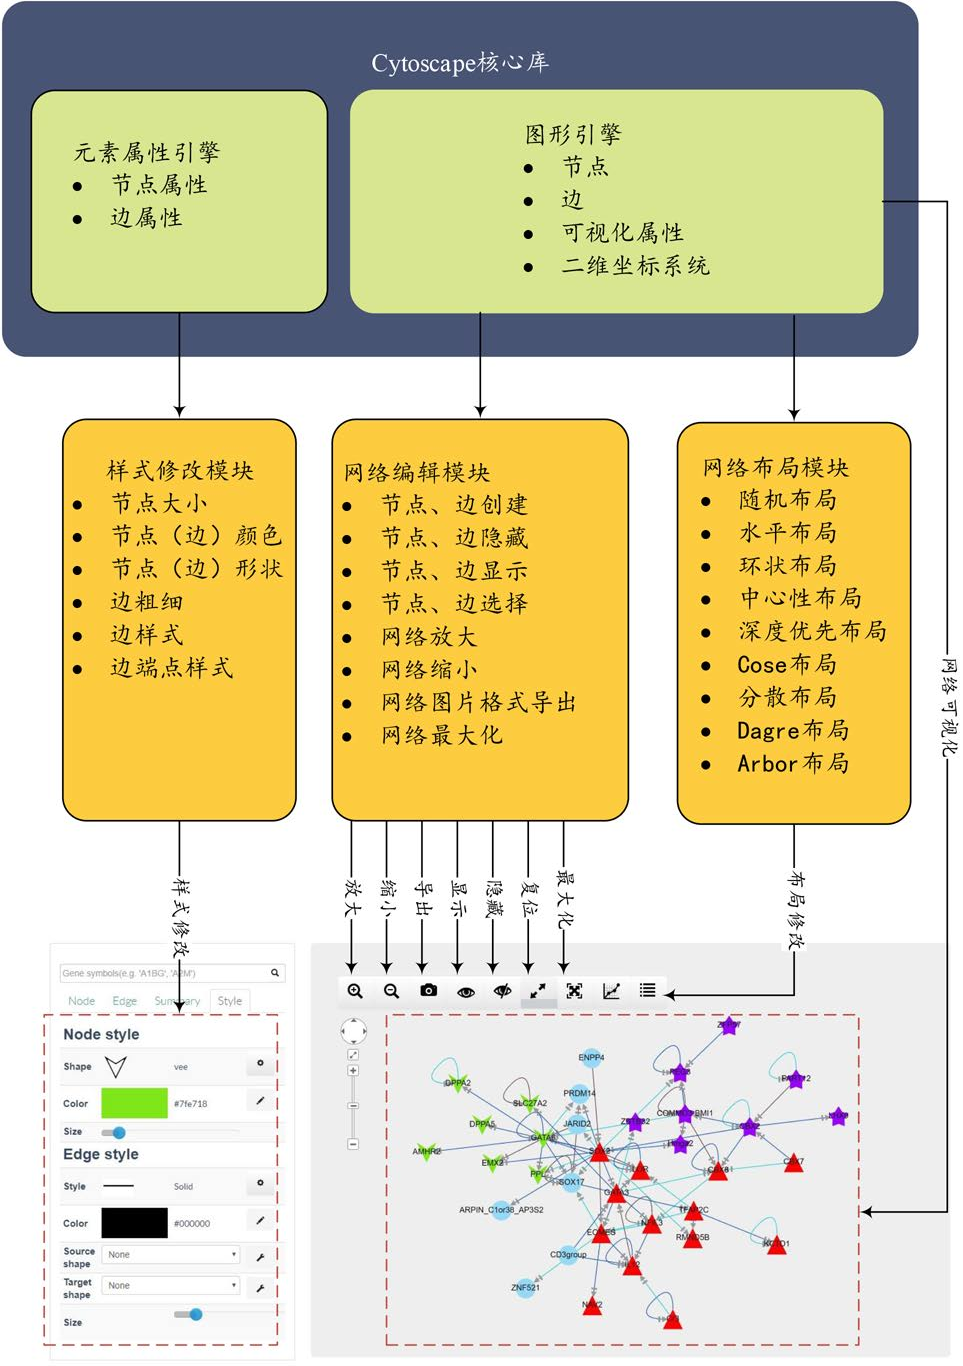
\includegraphics[width = 0.65\textwidth]{versioframework}
\caption[fig33]{可视化技术框架图}
\label{fig33}
\end{figure}

\section{本章小结}
在传统的生物通路网络一般是由生物学专家来绘制,数据库中展示的生物通路图也是静态的不可以编辑的。这种方式很耗时耗力,当发现一个通路中有新的信息时候,更新生物通路十分耗时。随着互联网技术发展和大数据时代的到来,数据的可视化技术日益成熟。互联网时代研究者对于数据的快速获取和分析需求日益增长。

本章介绍了我们开发的一款基于Cytoscape可视化技术的生物通路网络可视化系统,该系统可以实现网络可视化、网络编辑、网络导出、网络中元素的样式修改、网络分析,同时该系统关联了基因、疾病、药物、通路、基因表达信息, 系统实现了以上这些丰富信息的融合。
